% !TEX TS-program = LuaLaTeX
\documentclass[11pt,compress,xcolor=x11names,UTF8]{beamer}
\usetheme{Boadilla}
\usecolortheme{seahorse}
\useinnertheme[shadow]{rounded}  
\useoutertheme[subsection=false]{smoothbars}
\usecolortheme{spruce}
\usecolortheme[named=SpringGreen4]{structure}
\usefonttheme{structurebold}
\useinnertheme{circles}
\usecolortheme{rose}
\usepackage{pifont}
\usepackage{academicons}
\usepackage{fontawesome}
\usepackage{iitem}
\usepackage{graphicx}
\usepackage{tabularx}
\setbeamertemplate{itemize item}{\ding{108}}
\setbeamertemplate{itemize subitem}{\ding{109}}
\setbeamertemplate{navigation symbols}{}
\setbeamercovered{transparent}  
\renewcommand\appendixname{附录}
\renewcommand\abstractname{摘要}
\graphicspath{{figure/}} % 图片路径
\usepackage{calligra} % Thank you
\usepackage{ctex} % 加入中文
%\setCJKsansfont{Noto Sans CJK SC}
\setsansfont{Lato} % Lato Roboto Fira Sans
\usepackage{makecell}
\newcommand{\tabincell}[2]{\begin{tabular}{@{}#1@{}}#2\end{tabular}}
\usepackage{url}					
\usepackage{natbib} % 参考文献
%\title[Spatial Generalized Linear Mixed Models]{Spatial Generalized Linear Mixed Models with Application to Prevalence Mapping}
\title{集装箱测试系统PDE的一种刻度方法}
%\subtitle{奖助金申请答辩}
\author[赵荣]{Email:zhaor25@mail2.sysu.edu.cn \and  } % \\ 专业:统计学 \\ 方向:数据分析与统计计算
\institute[中山大学]{School of Physics\and } % 理学院\\
\date[\today]{
\includegraphics[width=.5\textwidth]{logo}}

\begin{document}

\maketitle

\begin{frame}{Outline}
\tableofcontents
\end{frame}

\section{背景简介}

%\subsection{研究意义}

\begin{frame}{现有的PDE评估方法}
%\textsf{例} \textbf{例}  \textit{例} 
% \texttt{例}  % 调出仿宋字体了
目前测试现场的PDE计算方法:
\begin{equation}
PDE={\color{red}PDE_c}\cdot f_{cs}+constant
\end{equation}
其中 $PDE_c$ 是集装箱自己的内部PDE结果,  $f_{cs}$ 是扫描站和集装箱之间的对应系数。\footnote{假设扫面站和集装箱的测试结果线性关联}
\vspace{.5cm}

$f_{cs}$ 可以通过拟合两套系统都测量过的PMT的PDE结果得到,并且随着测量PMT的增加这个拟合系数会更加精确。\footnote{统计误差减小} 
%\begin{table}[]  
%\caption{PMT typical performance}  
%\resizebox{.8\textwidth}{!}{%
%\begin{tabular*}{.98\textwidth}{l|cccc}
%%\toprule  
%\hline  
%\hline  
%Performance & PDE &DCR & TTS& uniformity \\  
%\hline  
%HAMAMATSU &  lower\% & 20 kHz& 3ns& worse \\  
%NNVT  & higher\% & 40kHz & 7ns& better \\  
%\hline  
%\end{tabular*}  
%%}
%\end{table} 
%\begin{figure}
%\centering
%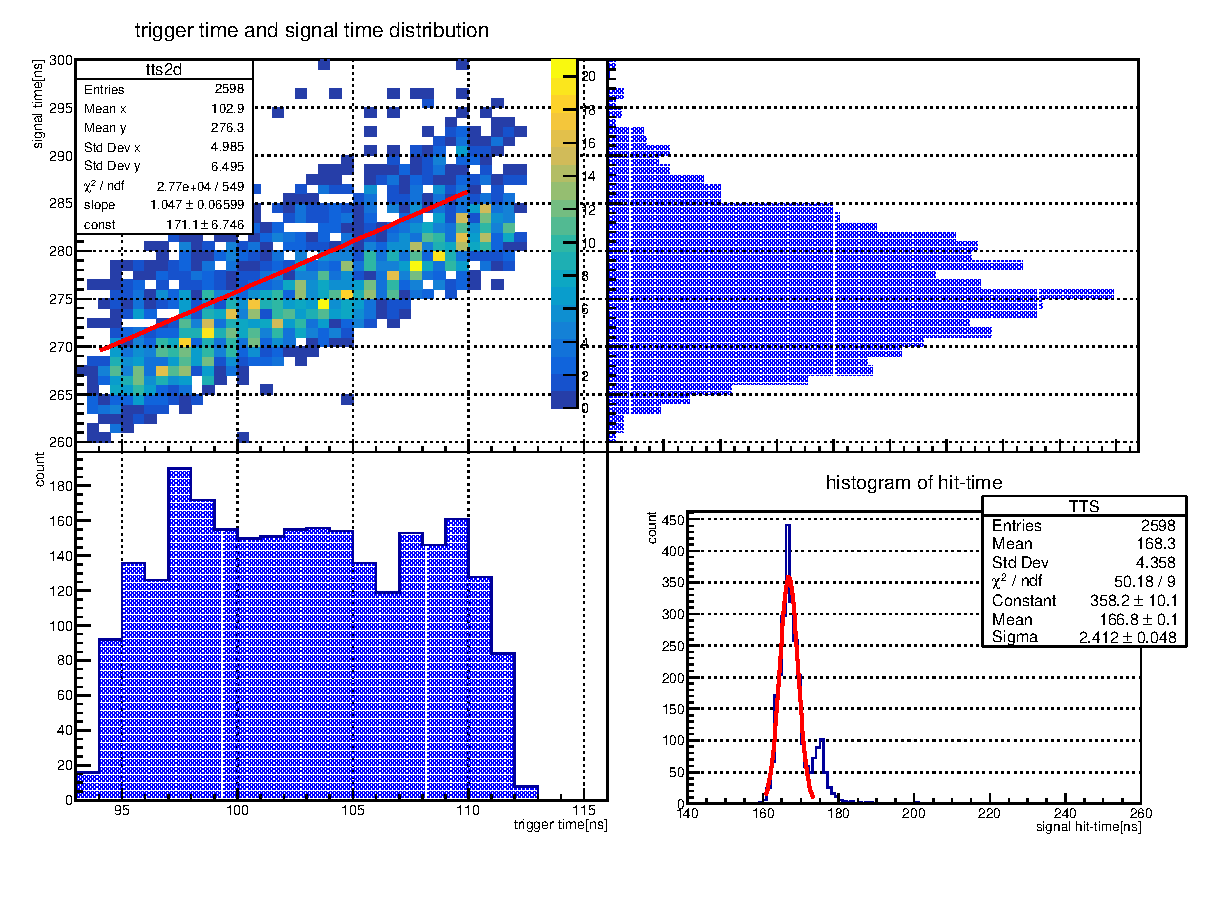
\includegraphics[width=0.78\textwidth]{typical_hittime} % 单图
%\end{figure}
\end{frame}
%%%%%%%%%%%%%%%%%%%%%%%%%%%%%%%%%%%%%%%%%%%
\begin{frame}{集装箱内部结果$PDE_{c}$的计算方法}
%\vspace{.5cm}
对于每一个测试抽屉, $PDE_c$ 的计算公式为:
\begin{equation}
PDE_c=\mu_{test}\cdot {\color{red}drawer_{factor}}
\label{pde_formula}
\end{equation}
其中 $\mu_{test}$ 是PMT测到的平均光子数,$drawer_{factor}$ 是抽屉因子,它将$\mu_{test}$ 转换到 $PDE_c$。

\vspace{.5cm}
\alert{因此计算 $PDE_c$之前需要对抽屉因子$drawer_{factor}$进行准确的刻度。}
\end{frame}
%%%%%%%%%%%%%%%%%%%%%%%%%%%%%%%%%%%%%%%%%%%
\begin{frame}{当前测试现场的刻度方法}
当前使用的方法\footnote{根据DocDB文档[https://juno.ihep.ac.cn/cgi-bin/Dev\_DocDB/ShowDocument?docid=3646]}是用15只滨松PMT在两个系统分别进行测试,再对测试结果进行拟合得到抽屉因子$drawer_{factor}$。

\vspace{.5cm}

另一种选择是,{\color{red}使用所有某个抽屉测量过的滨松PMT以及厂家数据对抽屉因子进行刻度。}\footnote{本文之后的数据都使用这种刻度方法}\\
\vspace{.5cm}
这样做的好处是:随着测量的PMT数量增加可以减少统计误差;\\
潜在的问题是:不同的抽屉用来刻度的PMT不相同。

\end{frame}
%%%%%%%%%%%%%%%%%%%%%%%%%%%%%%%%%%%%%%%%%%%
%\begin{frame}{calibration of each drawer}
%Generally, we put several PMTs with known PDE value\footnote{or QE value}  into one drawer and linearly fit the PDE-$\mu_{test}$ data to get \alert{drawer$_{factor}$}. 
%\vspace{.5cm}
%\hrule{\textwidth}
%\vspace{.5cm}
%
%While an alternative way to access the drawer$_{factor}$ is fitting PDE-$\mu_{test}$ data {\color{red}from all the PMTs tested in one drawer rather than the mannual selected ones.} Then once we finish one PMT test in a drawer we will get one more statistical sample in the PDE-$\mu_{test}$ fitting, and we could expect that the fitted drawer$_{factor}$ will get more stable as we testing more PMTs.
%
%\vspace{.5cm}
%The advantage of this "self-calibration" method is that we could {\color{red}decrease the statistical error as much as possible}; and the remained fluctuation of drawer$_{factor}$ can be the system error. 
%\end{frame}
\section{集装箱抽屉的刻度}
%%%%%%%%%%%%%%%%%%%%%%%%%%%%%%%%%%%%%%%%%%%
\begin{frame}{抽屉刻度方法}
滨松厂家提供部分PMT的QE\footnote{假定所有的PMT的收集效率相同}值,可以从PMT数据库\footnote{王俊[http://pmtdb.juno.ihep.ac.cn/index.html]}查询到。如果某一个抽屉测到的滨松PMT恰好有QE的厂家值,就选用它进行刻度。

\vspace{.5cm}
\hrule{\textwidth}
\vspace{.5cm}
为了保证刻度PMT的性能,只选取通过集装箱测试的PMT进行刻度。
\end{frame}
%%%%%%%%%%%%%%%%%%%%%%%%%%%%%%%%%%%%%%%%%%%
\begin{frame}{一个抽屉的刻度结果}
随着测试PMT数量的增加,拟合统计误差逐渐减小,$drawer_{factor}$的拟合结果趋于稳定(更多抽屉拟合结果见back-up部分)。
\begin{figure}
\centering
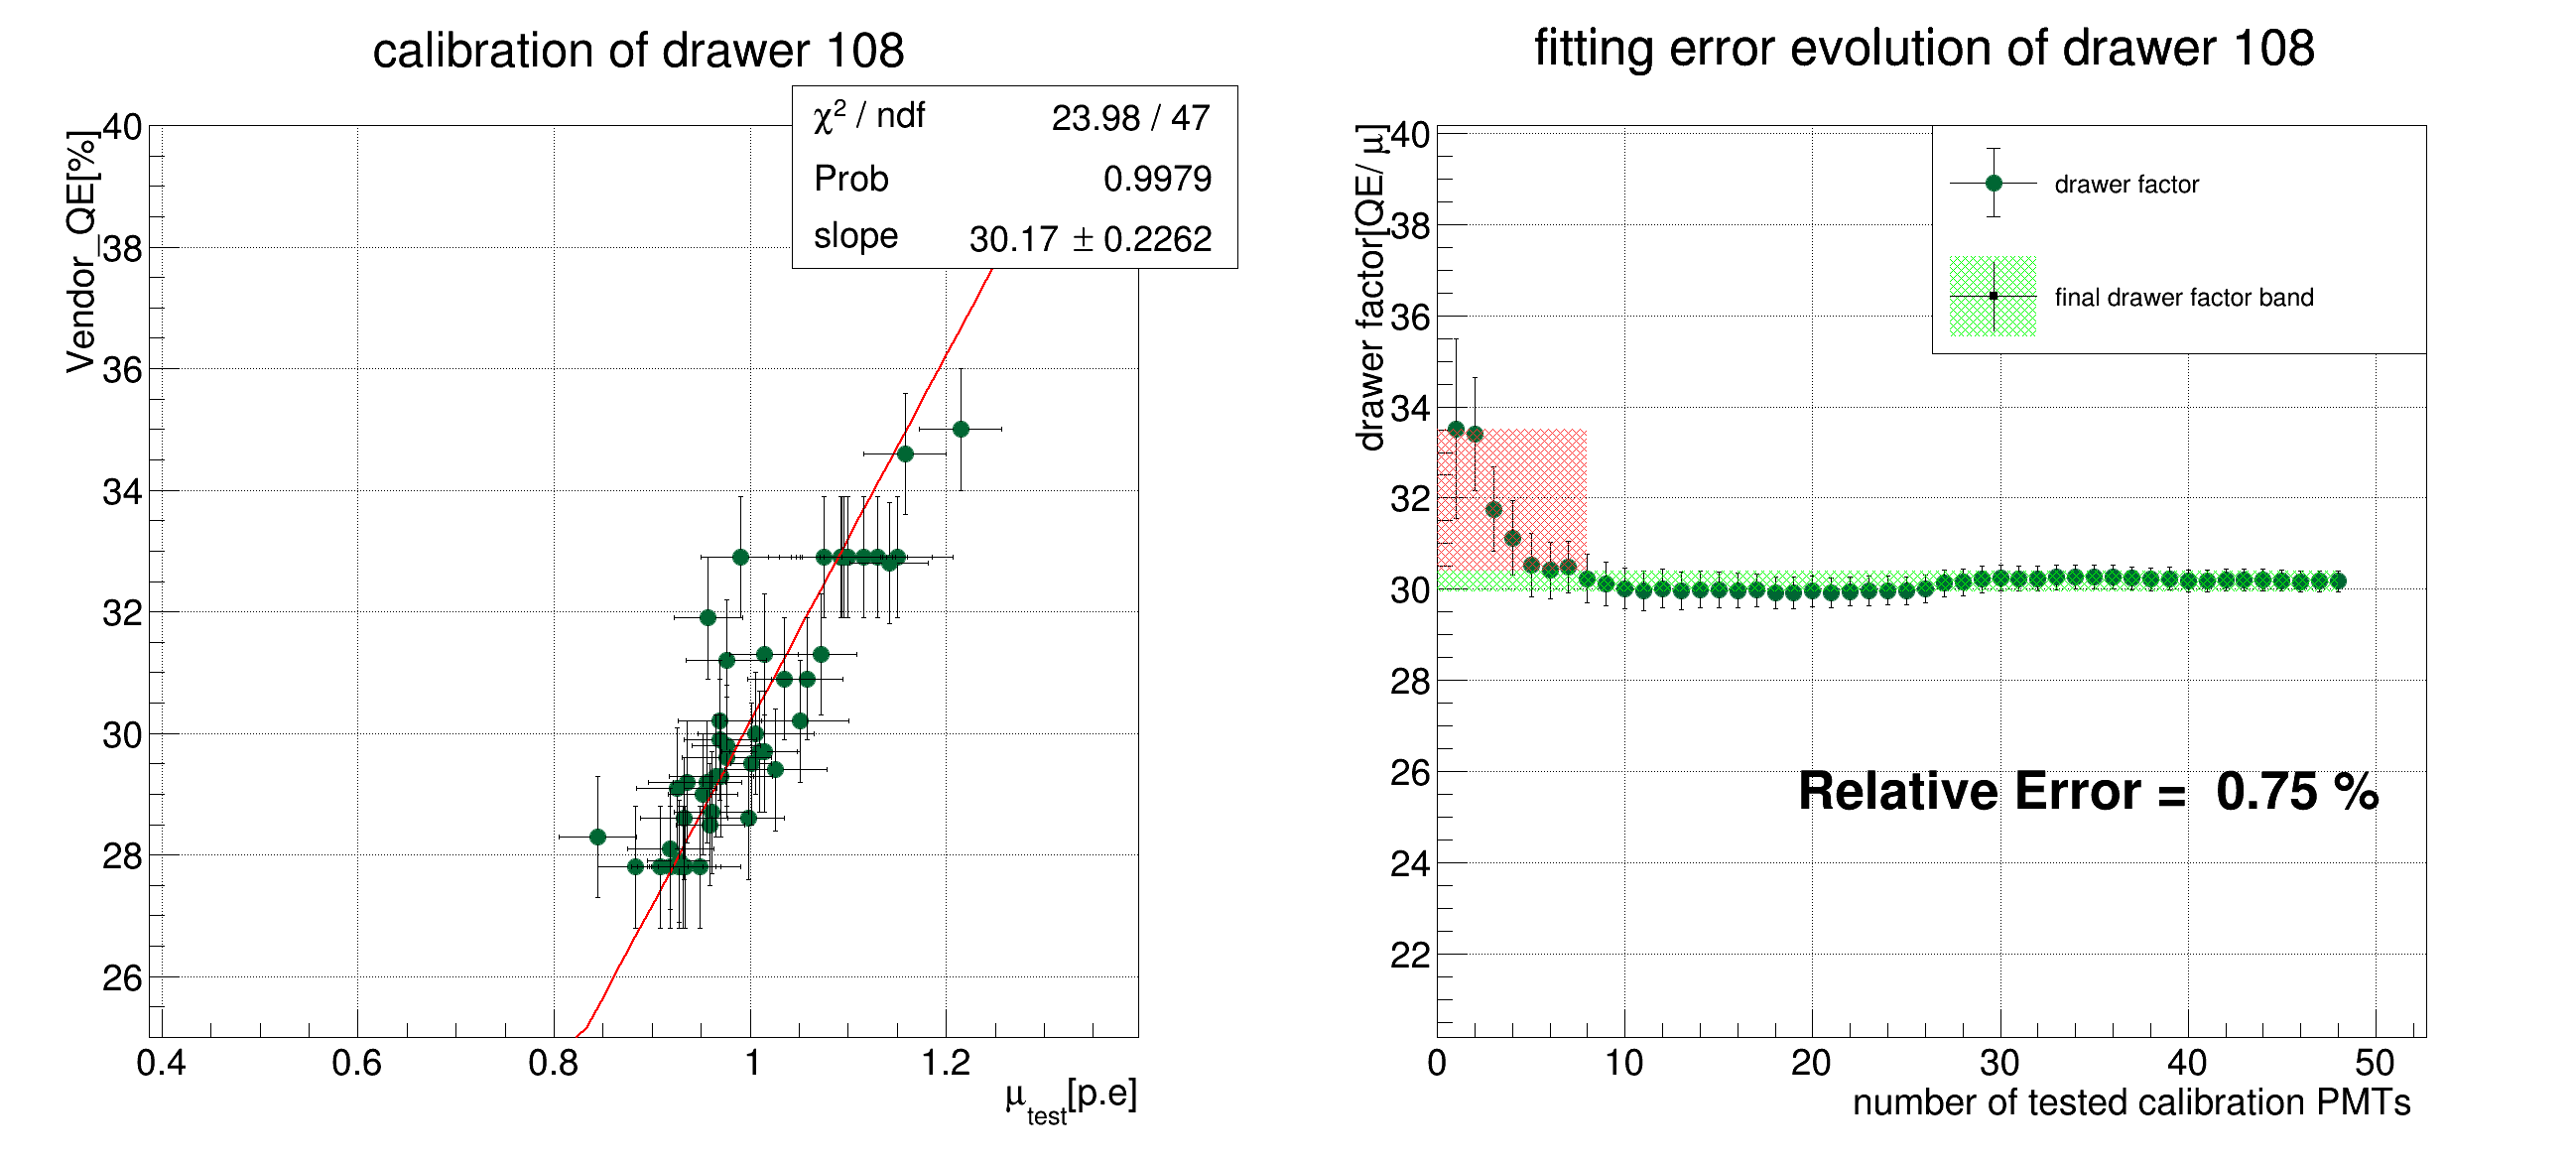
\includegraphics[width=0.98\textwidth]{sta101-7} % 单图
\caption{108抽屉的$drawer_{factor}$拟合结果}
\end{figure}
\end{frame}
%%%%%%%%%%%%%%%%%%%%%%%%%%%%%%%%%%%%%%%%%%%
%~~!!!!!!!!!!!!!!!!!!put two figures to illustrate!!!!!
\begin{frame}{抽屉刻度结果分析\footnote{拟合出的抽屉因子与现场所使用的抽屉因子的关联见back-up部分}}
\begin{columns}
\begin{column}{.5\textwidth}
\begin{figure}
\centering
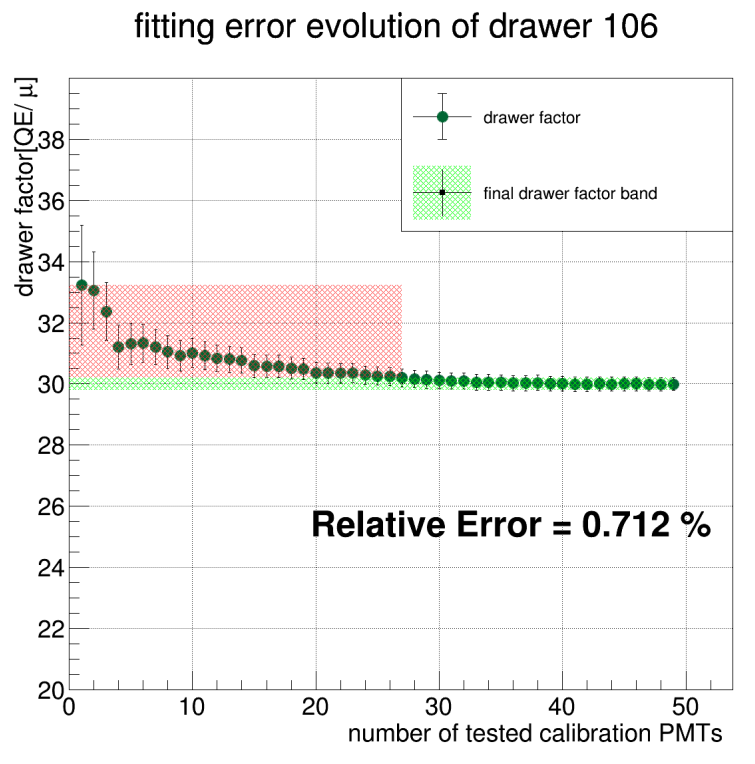
\includegraphics[width=\textwidth]{lt106} % 单图
\end{figure}
\end{column}
\begin{column}{.45\textwidth}
在某些通道拟合结果会随着时间缓慢上升或者下降(大约1\%),这说明光源强度出现了系统性的漂移。

\vspace{.5cm}
\hrule{\textwidth}
\vspace{.5cm}

\alert{所有抽屉的$drawer_{factor}$拟合误差都小于1\%}。

\vspace{.5cm}
\hrule{\textwidth}
\vspace{.5cm}

另一方面,这样的刻度方法可以用来监控系统的稳定性。因为如果系统稳定工作,拟合系数应该随机涨落。

\end{column}
\end{columns}
\end{frame}
%%%%%%%%%%%%%%%%%%%%%%%%%%%%%%%%%%%%%%%%%%%
%~~!!!!!!!!!!!!!!!!!!put two figures to illustrate!!!!!
%\begin{frame}{抽屉刻度结果分析\footnote{拟合出的抽屉因子与现场所使用的抽屉因子的关联见back-up部分}}
%\begin{columns}
%\begin{column}{.5\textwidth}
%\begin{figure}
%\centering
%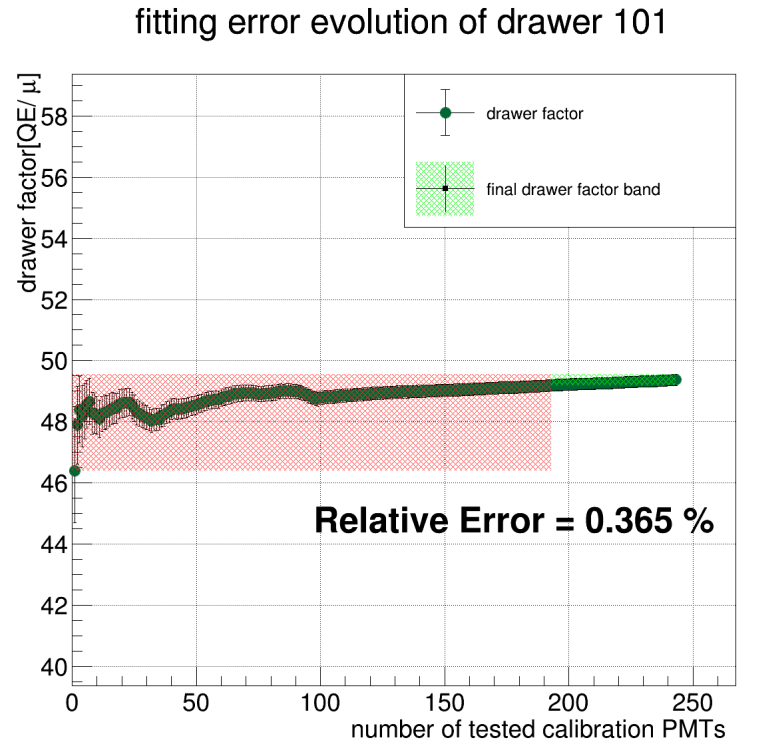
\includegraphics[width=\textwidth]{lt101} % 单图
%\end{figure}
%\end{column}
%\begin{column}{.45\textwidth}
%101抽屉一直放置参考PMT EA0419,抽屉因子$drawer_{factor}$拟合的结果随着时间漂移,这存在两种可能:
%\vspace{.5cm}
%
%\hrule{\textwidth}
%\vspace{.5cm}
%
%另一方面,这样的刻度方法可以用来监控系统的稳定性。因为如果系统稳定工作,拟合系数应该随机涨落。
%
%\end{column}
%\end{columns}
%\end{frame}
%%%%%%%%%%%%%%%%%%%%%%%%%%%%%%%%%%%%%%%%%%%
%~~!!!!!!!!!!!!!!!!!!put two figures to illustrate!!!!!
\begin{frame}{抽屉刻度结果分析}
\begin{columns}
\begin{column}{.5\textwidth}
\begin{figure}
\centering
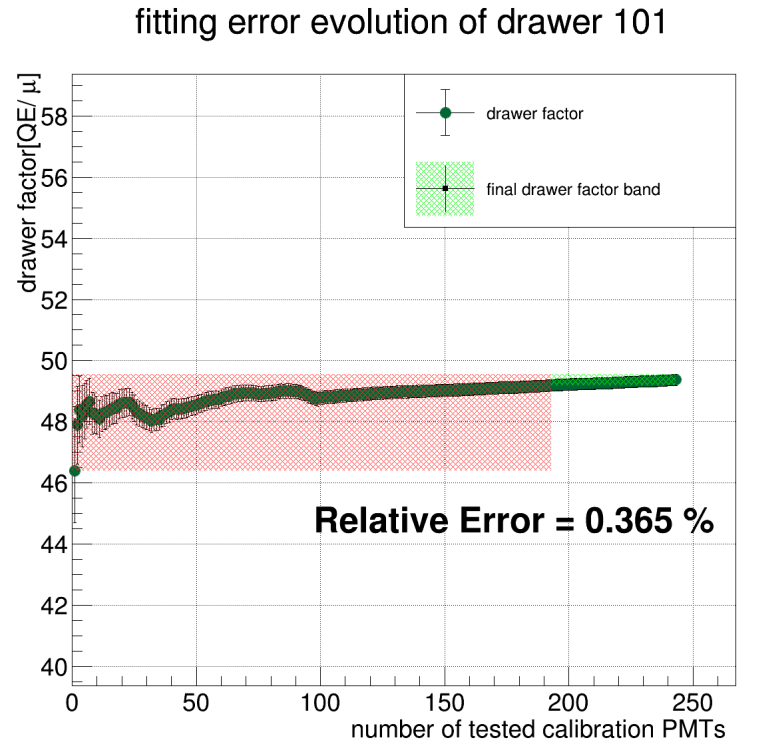
\includegraphics[width=\textwidth]{lt101} % 单图
\end{figure}
\end{column}
\begin{column}{.45\textwidth}
101抽屉一直放置参考PMT EA0419,抽屉因子$drawer_{factor}$拟合的结果随着时间漂移,这存在两种可能:
\vspace{.5cm}
\hrule{\textwidth}
\vspace{.5cm}
\begin{itemize}
\item 光源光强随时间变化(光强减小)
\item PMT自身的性能PDE在减小
\end{itemize}

\end{column}
\end{columns}
\end{frame}
\section{PDE的计算}
%%%%%%%%%%%%%%%%%%%%%%%%%%%%%%%%%%%%%%%%%%%
\begin{frame}{$PDE$的计算}
根据公式\ref{pde_formula},通过$\mu_{test}$以及抽屉因子即可算出集装箱自己的PDE结果$PDE_c$。假设集装箱系统和扫描站对同一只PMT的测量结果是正比关系\footnote{参考王俊和王耀光的模拟结果},通过拟合线性参数$f_{cs}$可以算出最终的PDE。
\vspace{.5cm}
\hrule{\textwidth}
\vspace{.5cm}

\begin{itemize}
%\item 因为MCP和HAMAMATSU 两种PMT的性能差异较大,需要对两种PMT分别计算$f_{cs}$。
\item 使用相同的系数拟合两种PMT,$f_{cs}$=0.897
\item MCP-PMT 的高量子效率PMT和之前的低量子效率PMT在两个系统的表现不同,需要更多的测量数据进行确认。
\end{itemize}
\end{frame}
%%%%%%%%%%%%%%%%%%%%%%%%%%%%%%%%%%%%%%%%%%%
%%%%%%%%%%%%%%%%%%%%%%%%%%%%%%%%%%%%%%%%%%%
\begin{frame}{两套装置测量结果的转换}
利用$PDE_c$和$PDE_s$对所有MCP-PMT拟合$f_{cs}$的结果\footnote{挑选条件:集装箱测试合格而且$\Delta PDE<5$}:
%\begin{columns}
%\begin{column}{\textwidth}
\begin{figure}
\centering
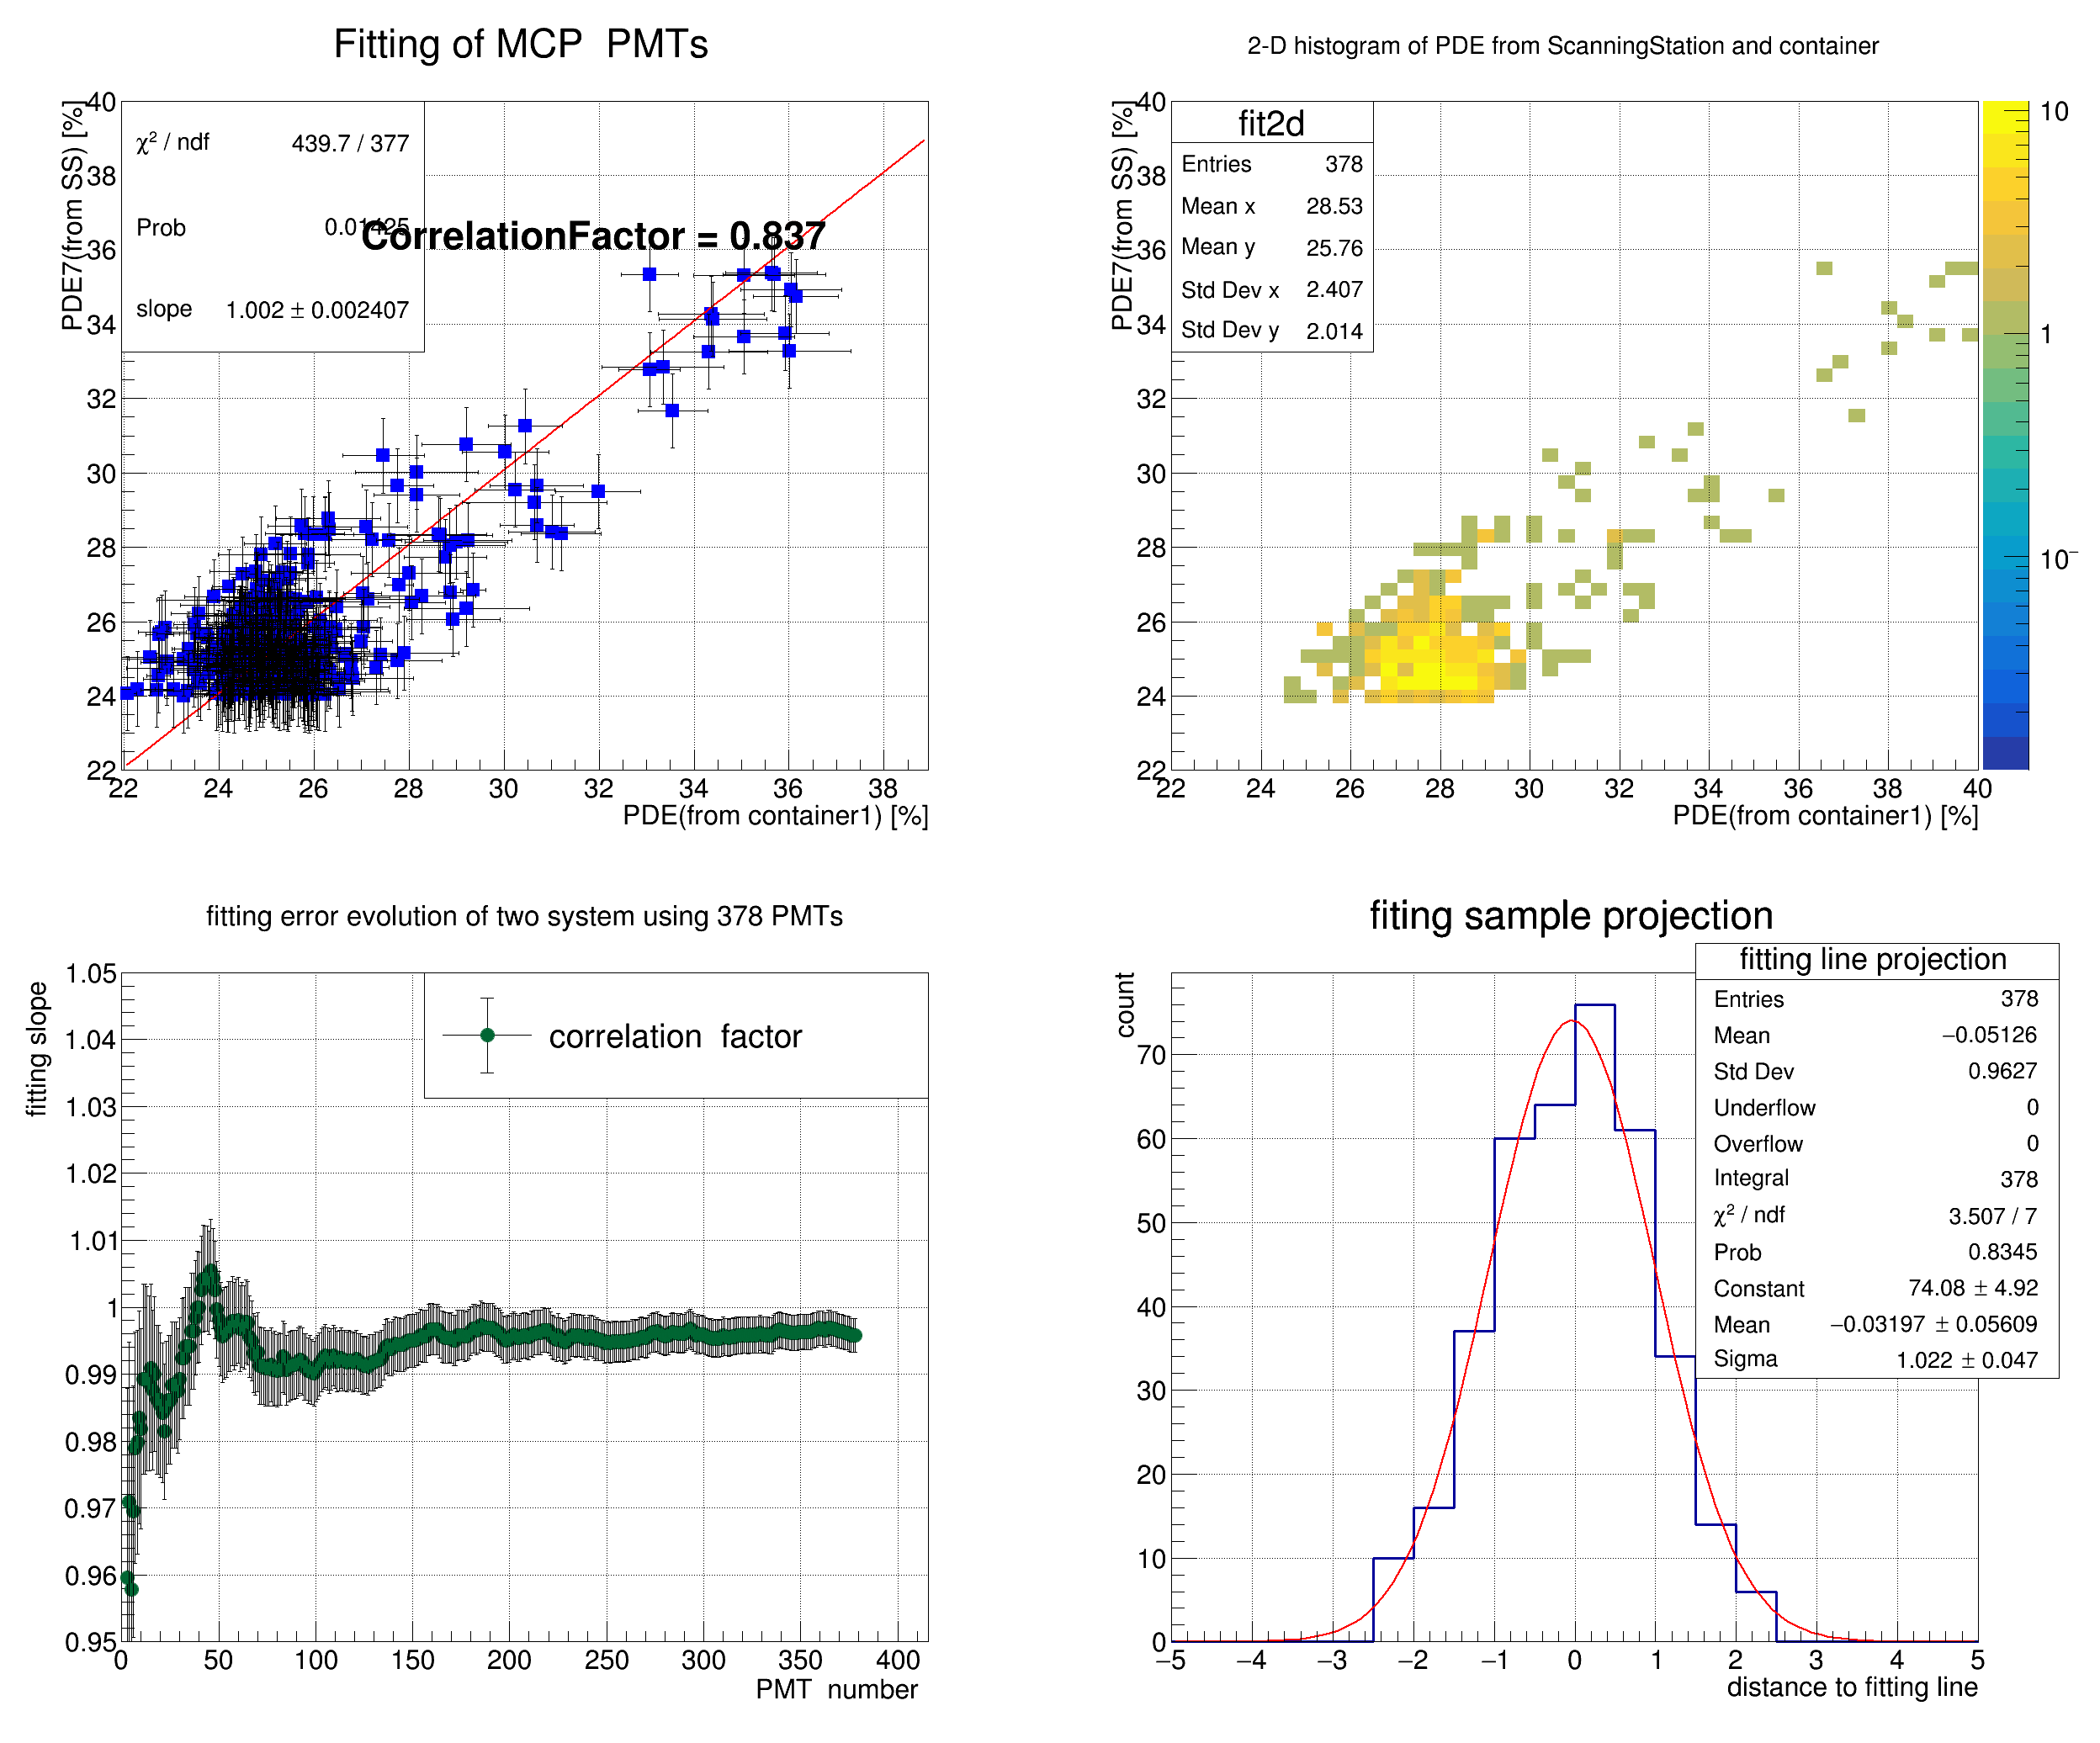
\includegraphics[width=0.58\textwidth]{fit_mcp_noint}
\end{figure}
%\end{column}
%\begin{column}{.001\textwidth}

%\end{column}
%\end{columns}
\end{frame}

%%%%%%%%%%%%%%%%%%%%%%%%%%%%%%%%%%%%%%%%%%%%%%%%%%%%%%%%%%%%%%%%%%%%
\begin{frame}{两套装置测量结果的转换}
利用$PDE_c$和$PDE_s$对所有HAMAMATSU-PMT拟合$f_{cs}$的结果\footnote{挑选条件:集装箱测试合格而且$\Delta PDE<5$}:
\begin{figure}
\centering
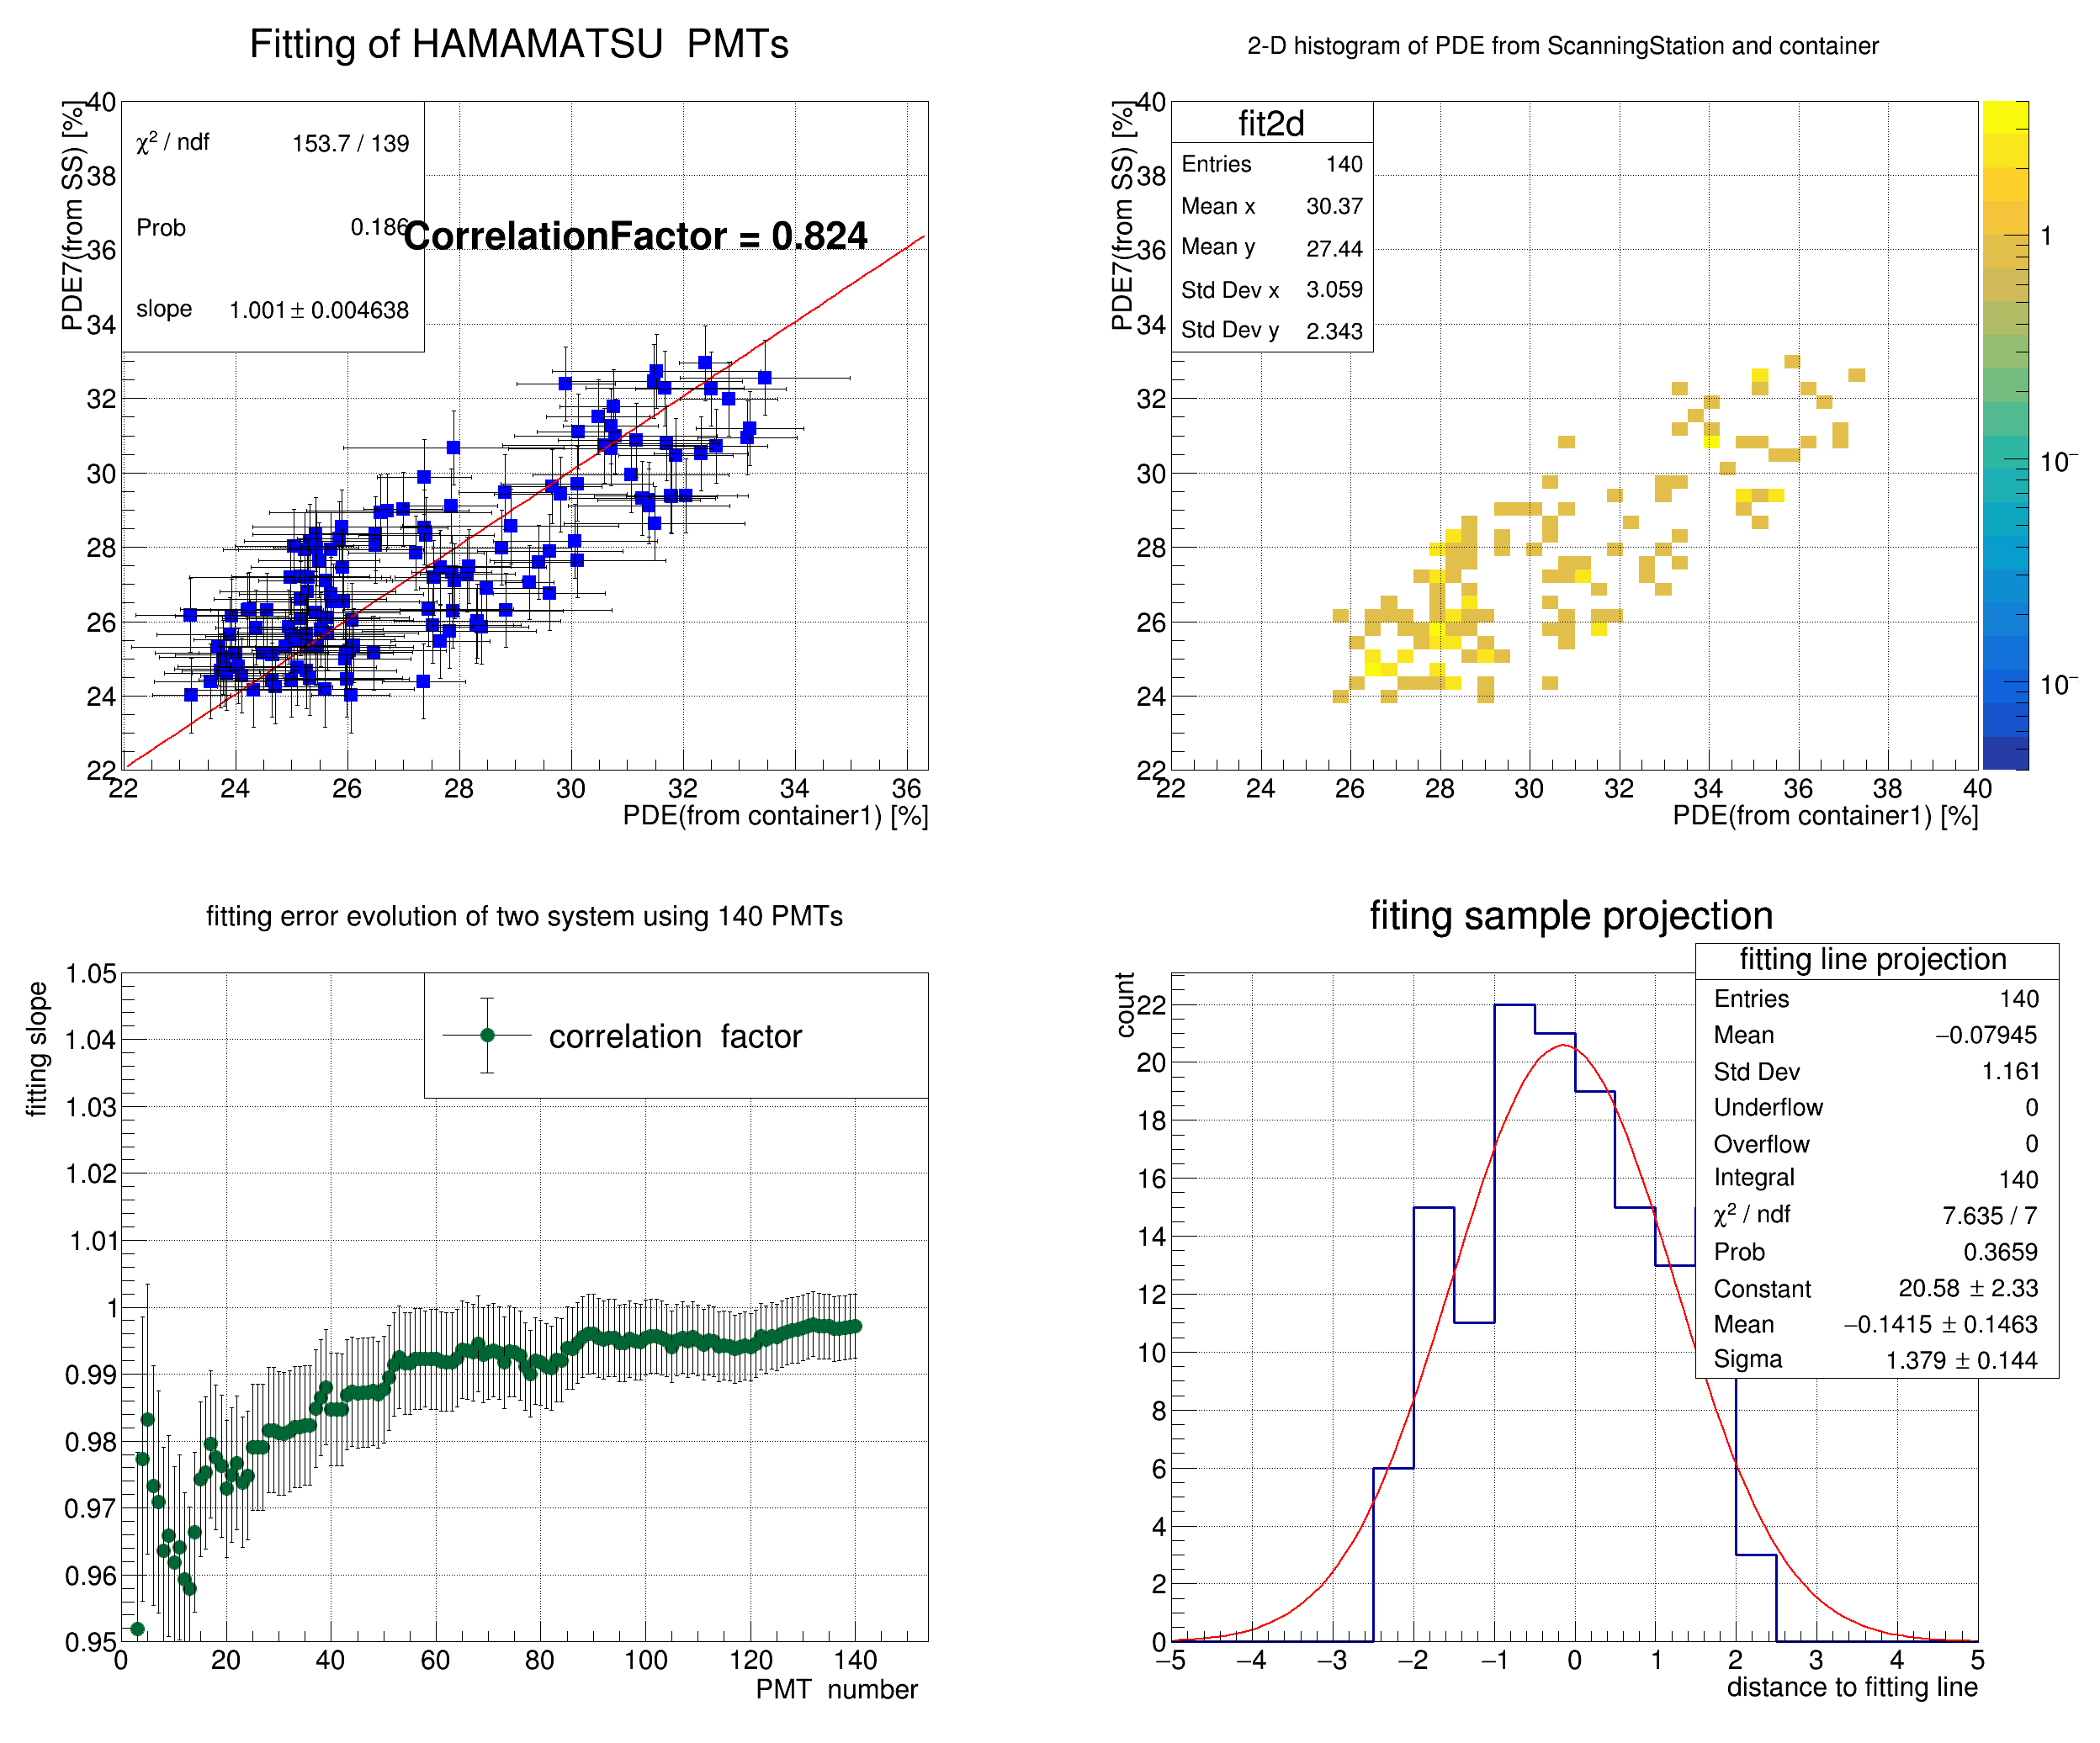
\includegraphics[width=0.58\textwidth]{fit_hmp_noint}
\end{figure}
\end{frame}
%%%%%%%%%%%%%%%%%%%%%%%%%%%%%%%%%%%%%%%%%%%%%%%%%%%%%%%%%%%%%%%%%%%%
\begin{frame}{两套装置测量结果的转换}
利用$PDE_c$和$PDE_s$对所有PMT拟合$f_{cs}$的结果\footnote{挑选条件:集装箱测试合格而且$\Delta PDE<5$}:
\begin{figure}
\centering
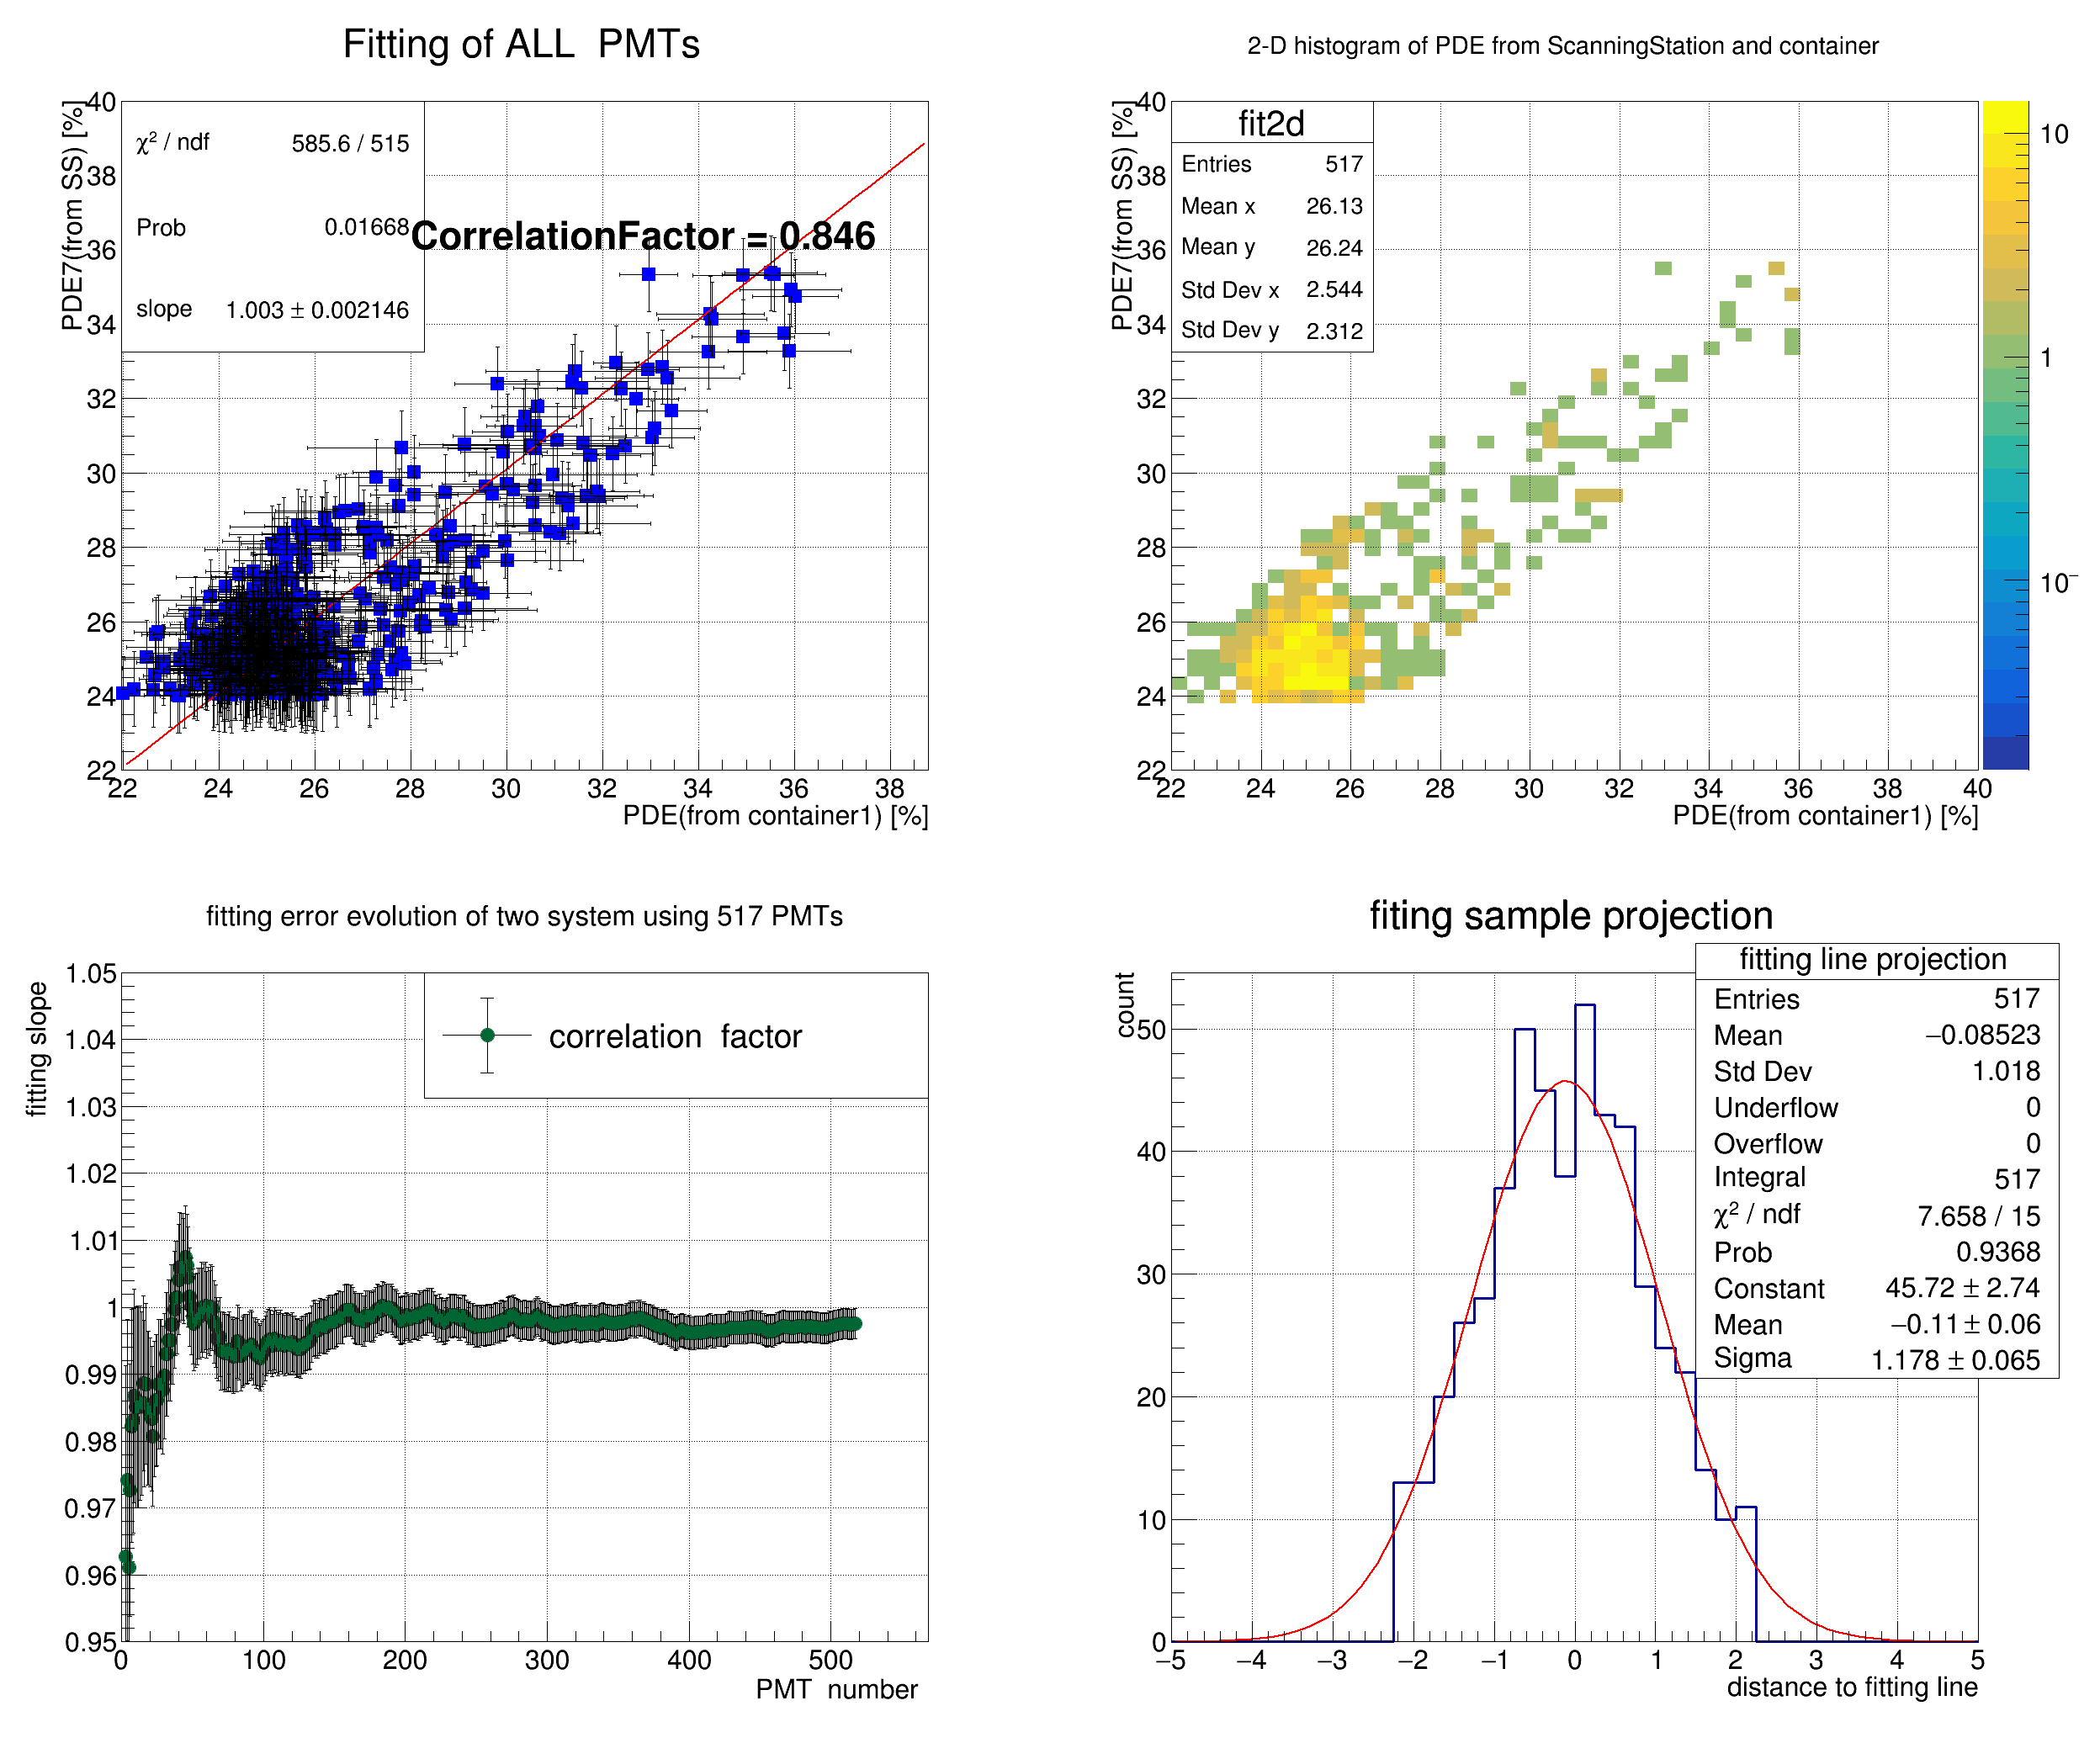
\includegraphics[width=0.58\textwidth]{fit_all_pmts}
\end{figure}
\end{frame}
%%%%%%%%%%%%%%%%%%%%%%%%%%%%%%%%%%%%%%%%%%%%%%%%%%%%%%%%%%%%%%%%%%%%
\begin{frame}{PDE计算结果}
根据$\mu_{test}$\footnote{$\mu_{test}$和现场结果的对比见BACK-UP部分}以及拟合得到的$drawer_{factor}$和$f_{cs}$可以计算集装箱最终的PDE测试结果:
\hrule{\textwidth}
\begin{figure}
\centering
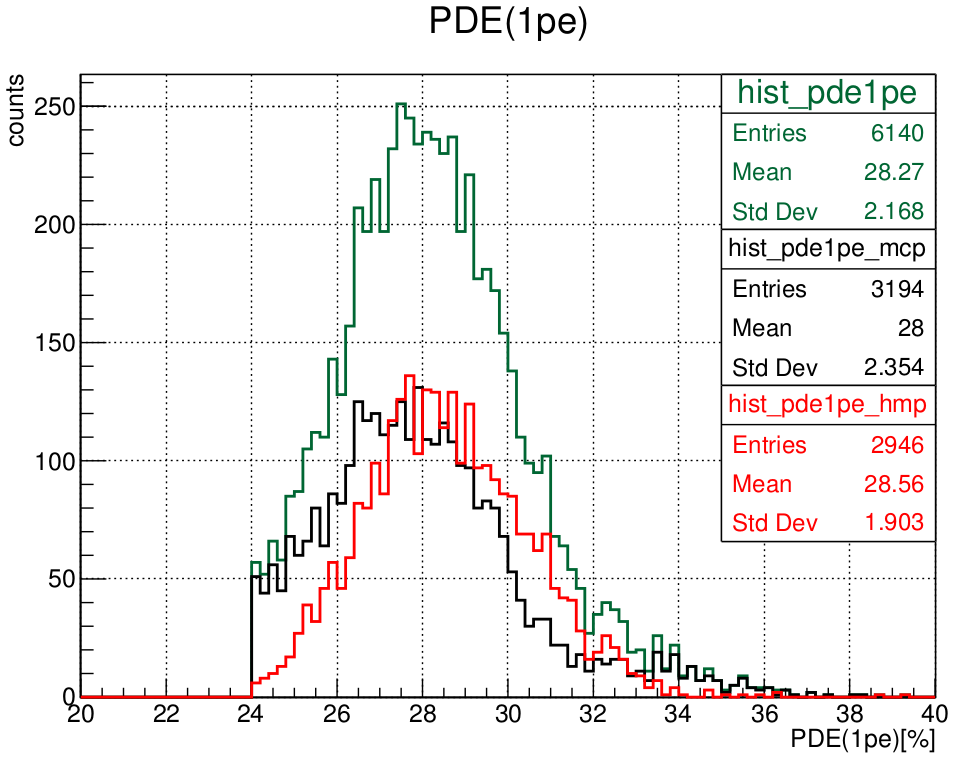
\includegraphics[width=0.45\textwidth]{pde_res}
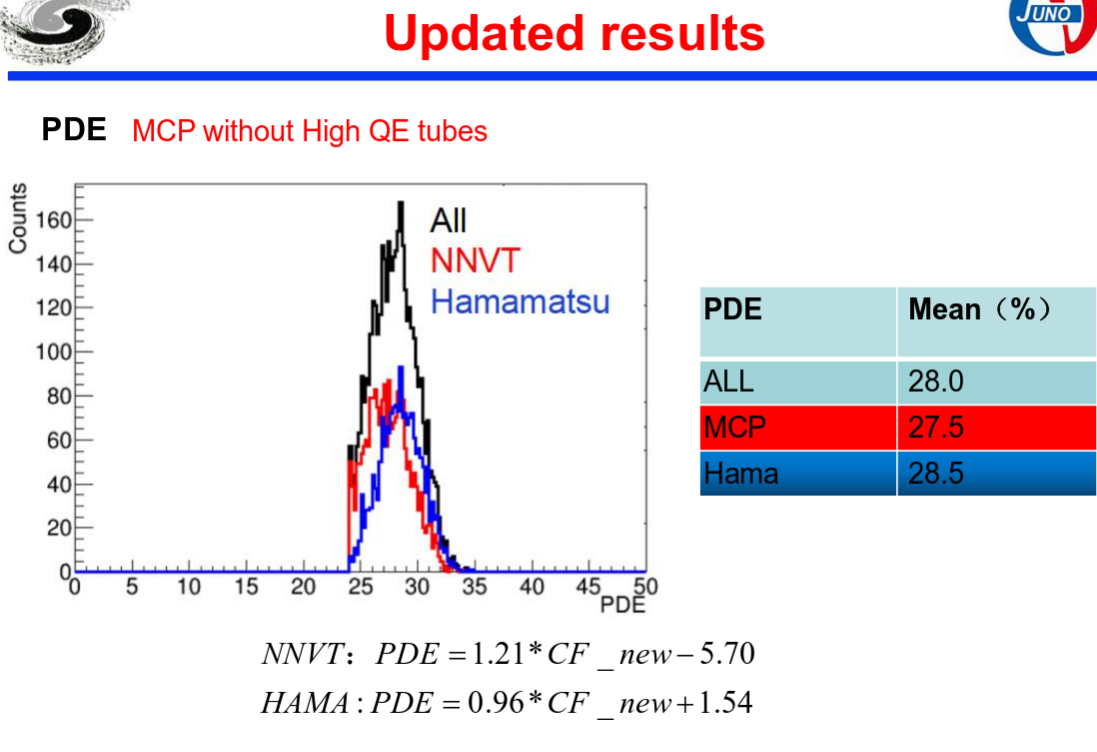
\includegraphics[width=0.45\textwidth]{hqpde}
\caption{左图是抽屉累积拟合的结果,右图是现场所使用刻度方法结果\footnote{https://juno.ihep.ac.cn/cgi-bin/Dev\_DocDB/ShowDocument?docid=3646}}
\end{figure}

\end{frame}
%%%%%%%%%%%%%%%%%%%%%%%%%%%%%%%%%%%%%%%%%%%%%%%%%%%%%%%%%%%%%%%%%%%%
\begin{frame}{PDE计算结果}
将MCP-PMT的高量子效率分开处理,统计集装箱1测量到的MCP-PMT的PDE结果\footnote{更新到2018-10-17的测试结果}:
%\hrule{\textwidth}
\begin{columns}
\begin{column}{.56\textwidth}
\begin{figure}
\centering
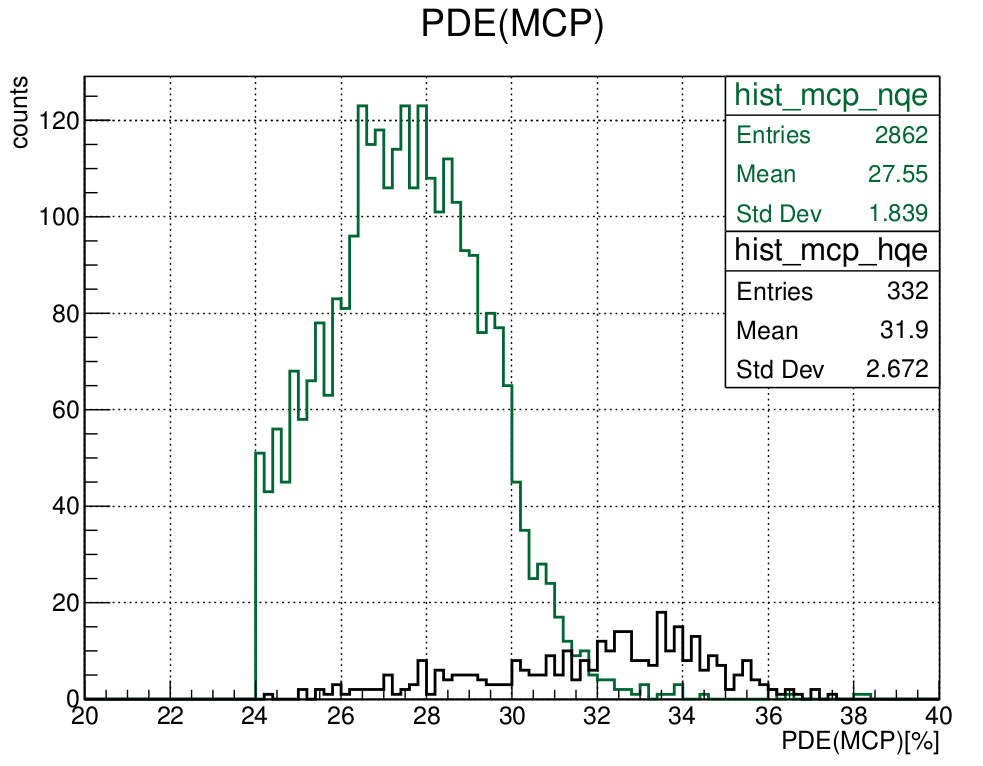
\includegraphics[width=\textwidth]{mcppde}
\end{figure}
\end{column}
\begin{column}{.4\textwidth}
\alert{MCP的高量子效率版本PDE相对增加了15.8\%}
\vspace{.5cm}
\hrule{\textwidth}
\vspace{.5cm}
PDE 的统计结果和现场算法得到的结果一致。\\
MCP:27.5\leftrightarrow \alert{27.55}\\
HAMAMATSU:28.5\leftrightarrow \alert{28.56}
\end{column}
%\end{figure}
\end{columns}
\end{frame}
%%%%%%%%%%%%%%%%%%%%%%%%%%%%%%%%%%%%%%%%%%%%%%%%%%%%%%%%%%%%%%%
%%%%%%%%%%%%%%%%%%%%%%%%%%%%%%%%%%%%%%%%%%%%%%%%%%%%%%%%%%%%%%%
\section{总结}

\begin{frame}{总结和结论}
\begin{itemize}
\item 使用抽屉自己的测量结果以及滨松厂家数据进行光强刻度,误差小于1\%。
\item 这种方法可以监控系统的稳定性,并且可以减小系统误差。
\item 基于上面的抽屉刻度结果计算集装箱PDE结果,与现场当前使用算法的结果一致(相对偏差小于1\%)。
\item MCP高量子效率版本的PMT,PDE相对提高15.78\%,平均值PDE=31.9\%\footnote{张海琼北京合作组会报告32.6\%}
\end{itemize}
\end{frame}

\begin{frame}
\centering {\zihao{0} \color{red} \calligra{谢谢}}
\end{frame}

\begin{frame}
\centering {\zihao{0} \color{red} \calligra{BACK-UP}}
\end{frame}

%\begin{frame}[allowframebreaks]
%\frametitle{References}
%\scriptsize
%\bibliographystyle{authordate1}
%\bibliography{R-GLMM-pkgs}
%\end{frame}

\appendix

\section*{附录}

\begin{frame}{其他重要参数的check}
HAMAMATSU-PMT的参数对比:

\vspace{.5cm}

\centering
\begin{tabular}{l|c|c}
\hline
\hline
参数(平均值)&  {\color{Blue} 我的结果} & {\color{Blue}测试现场结果} \\\hline
暗计数(kHz)&17.8&16.6\\
信号上升时间(ns)&7.3& 6.9\\
信号下降时间(ns)&10.36& 10.2\\
峰谷比&3.3& 3.9\\
分辨率&0.28& 0.277\\
高压(V)&1861& 1858\\
信号半高宽(ns)&9.08& 11.6\\
\hline
\end{tabular}

%\begin{table}[htbp]  
%\caption{PMT typical performance}  
%\resizebox{.8\textwidth}{!}{%
%\begin{tabular*}{.98\textwidth}{l|cccc}
%%\toprule  
%\hline  
%\hline  
%Performance & PDE &DCR & TTS& uniformity \\  
%\hline  
%HAMAMATSU &  lower\% & 20 kHz& 3ns& worse \\  
%NNVT  & higher\% & 40kHz & 7ns& better \\  
%\hline  
%\end{tabular*}  
%%}
%\end{table} 

\end{frame}
\begin{frame}{其他重要参数的check}
MCP-PMT的参数对比:

\vspace{.5cm}

\centering
\begin{tabular}{l|c|c}
\hline
\hline
参数(平均值)&  {\color{Blue} 我的结果} & {\color{Blue}测试现场结果} \\\hline
暗计数(kHz)&41.4&44.3\\
信号上升时间(ns)&3.2& 4.6\\
信号下降时间(ns)&15.9& 16.2\\
峰谷比&3.19& 4.4\\
分辨率&0.35& 0.32\\
高压(V)&1783& 1784\\
信号半高宽(ns)&5.8& 7.7\\
\hline
\end{tabular}
\end{frame}
\begin{frame}{drawer-calibration}
\vspace{-.5cm}
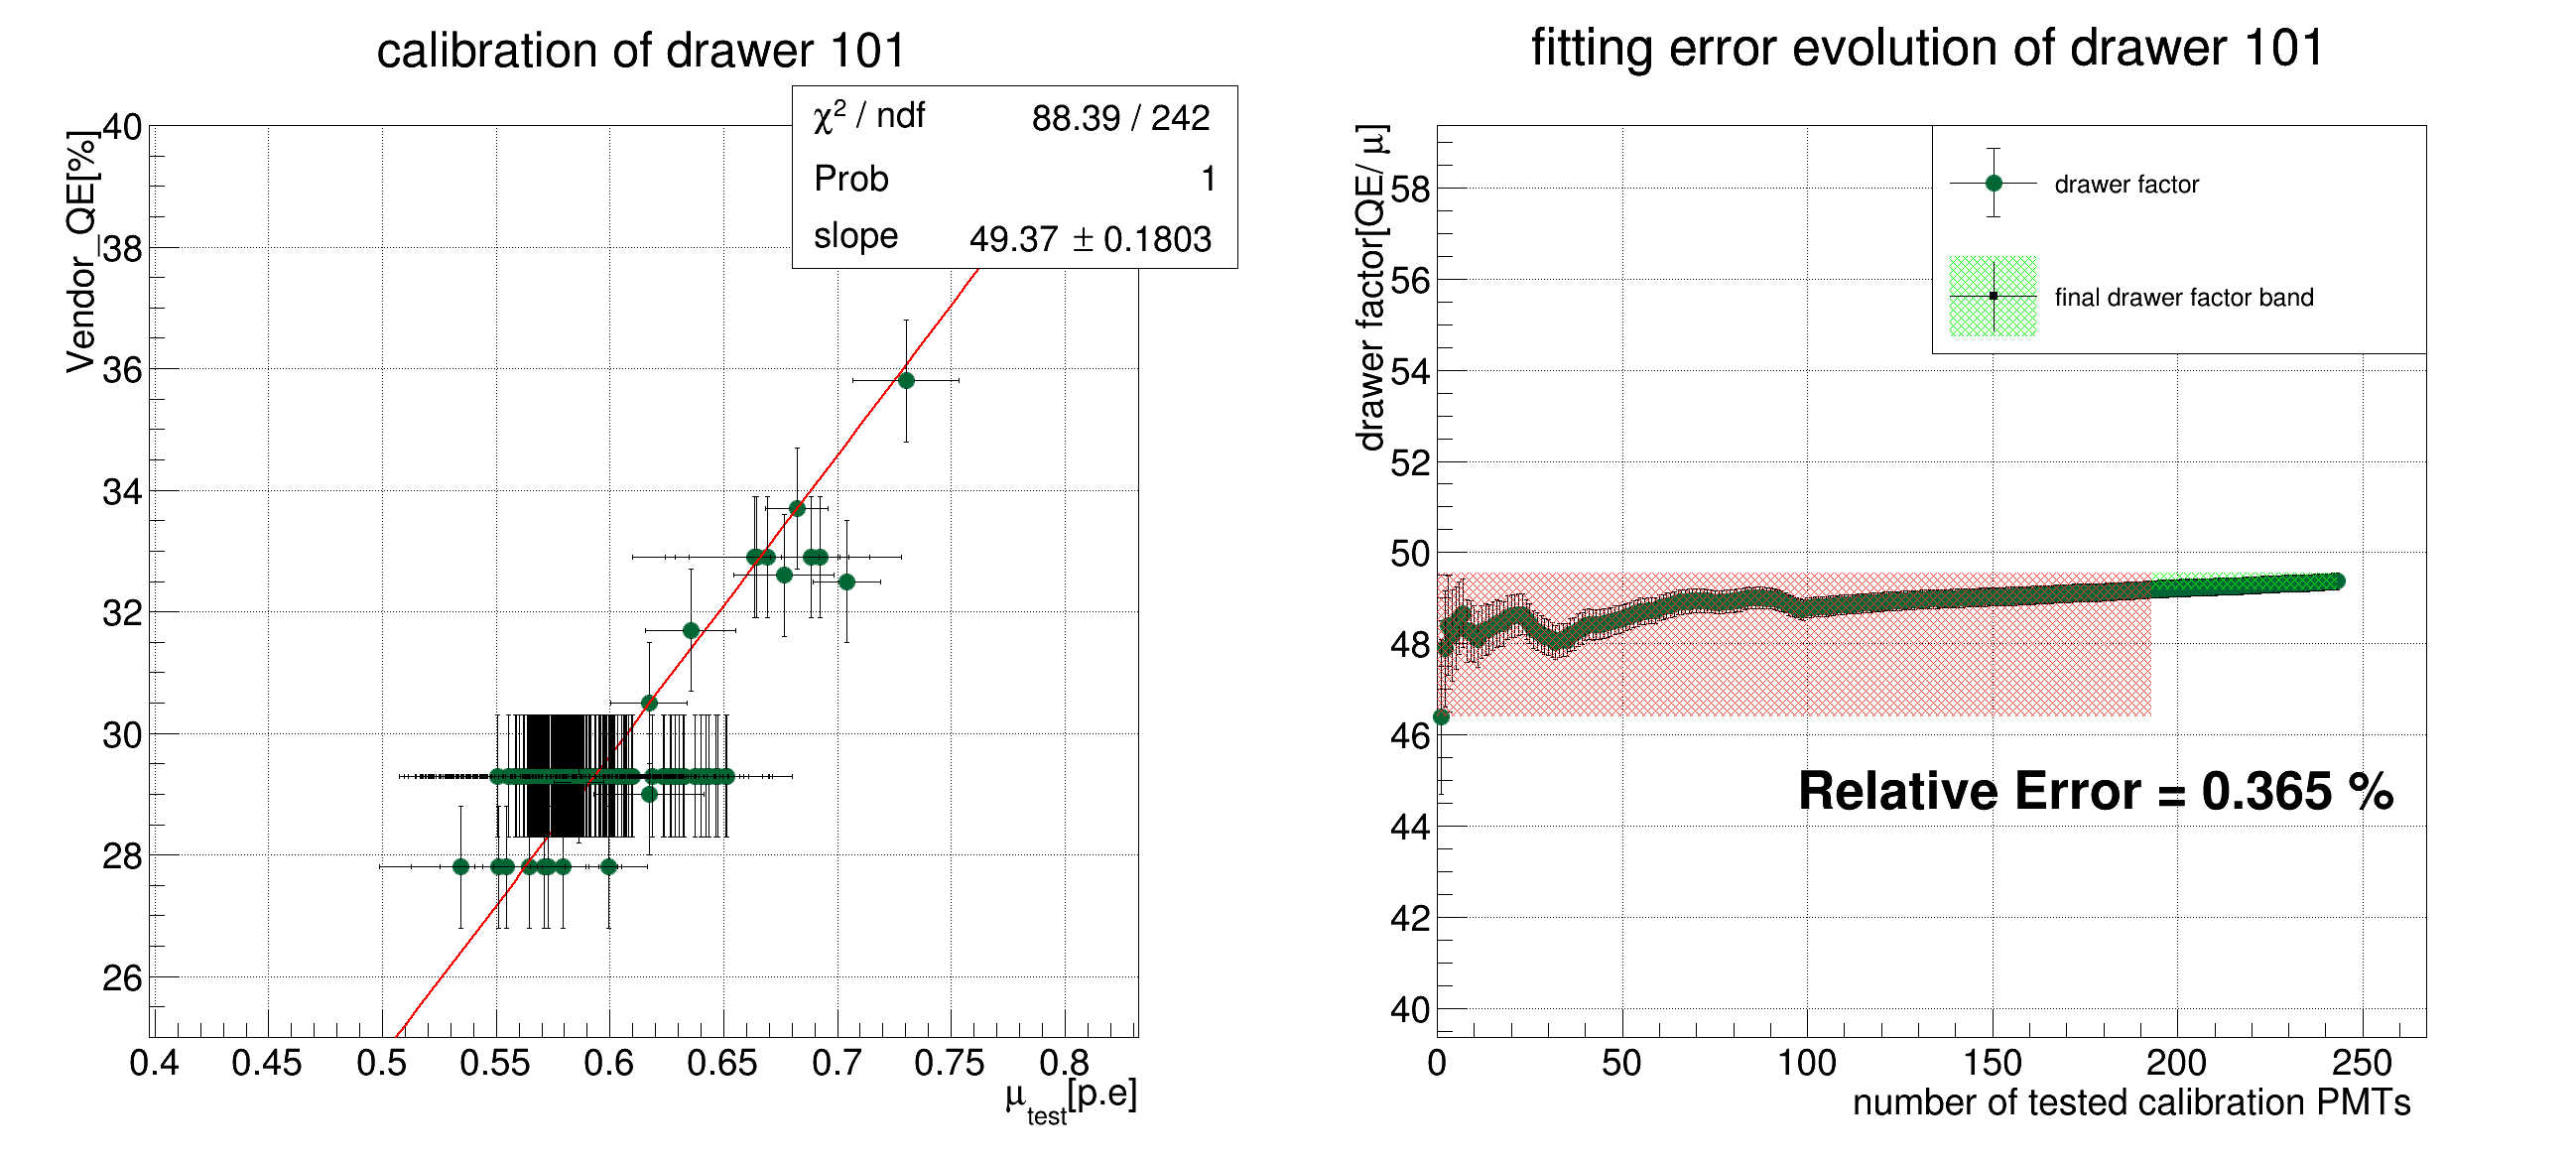
\includegraphics[width=0.45\textwidth]{sta101-0} 
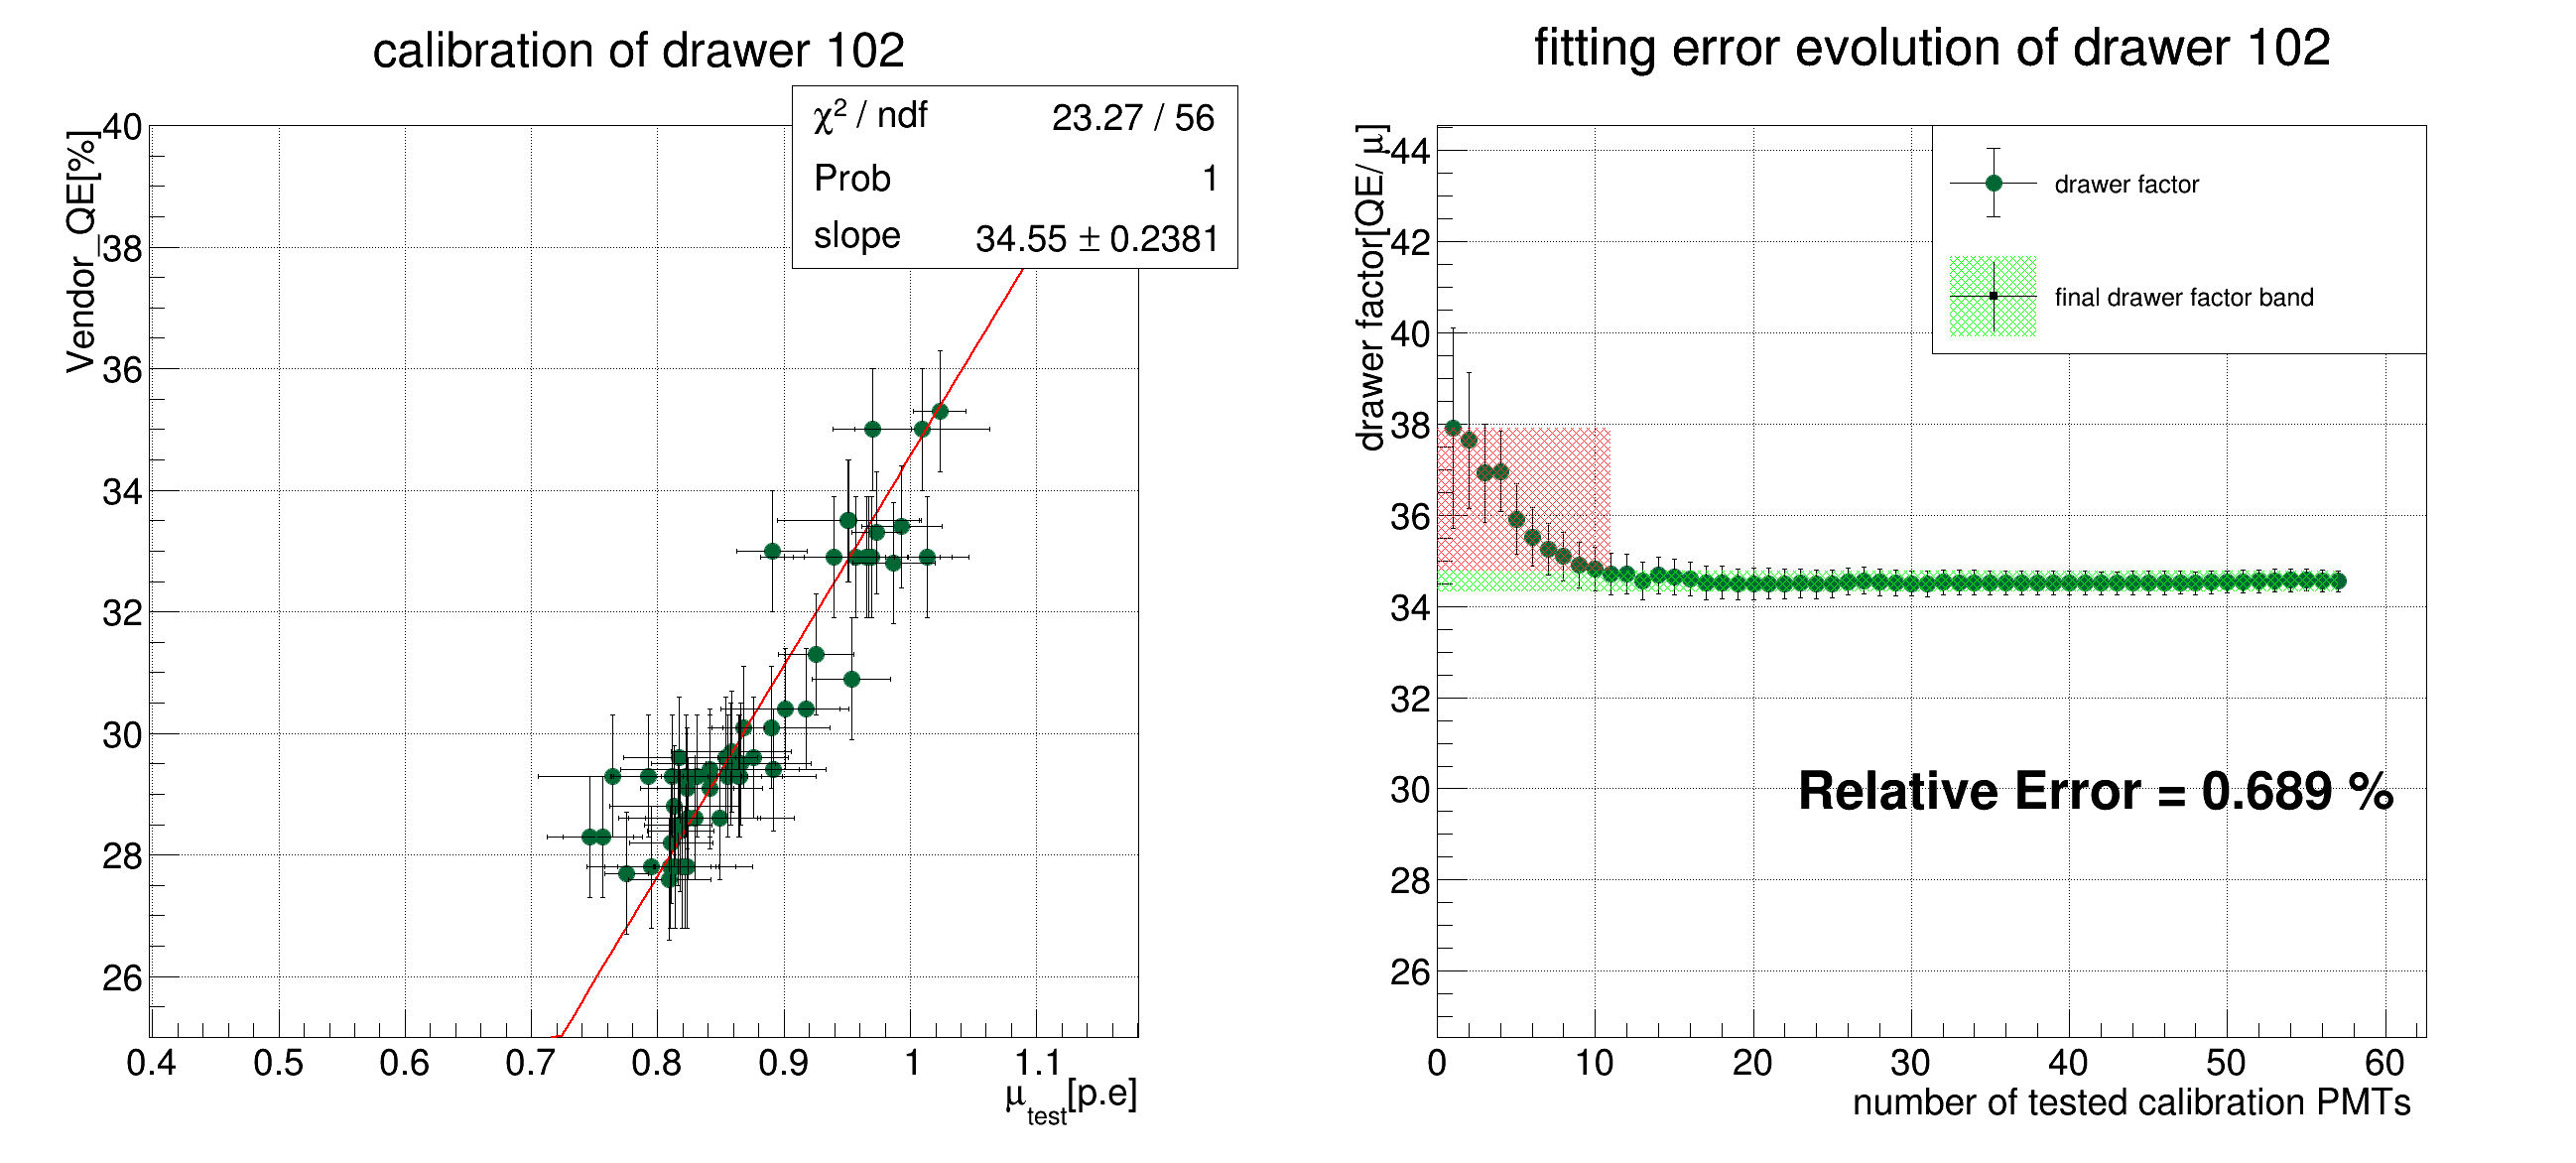
\includegraphics[width=0.45\textwidth]{sta101-1} 
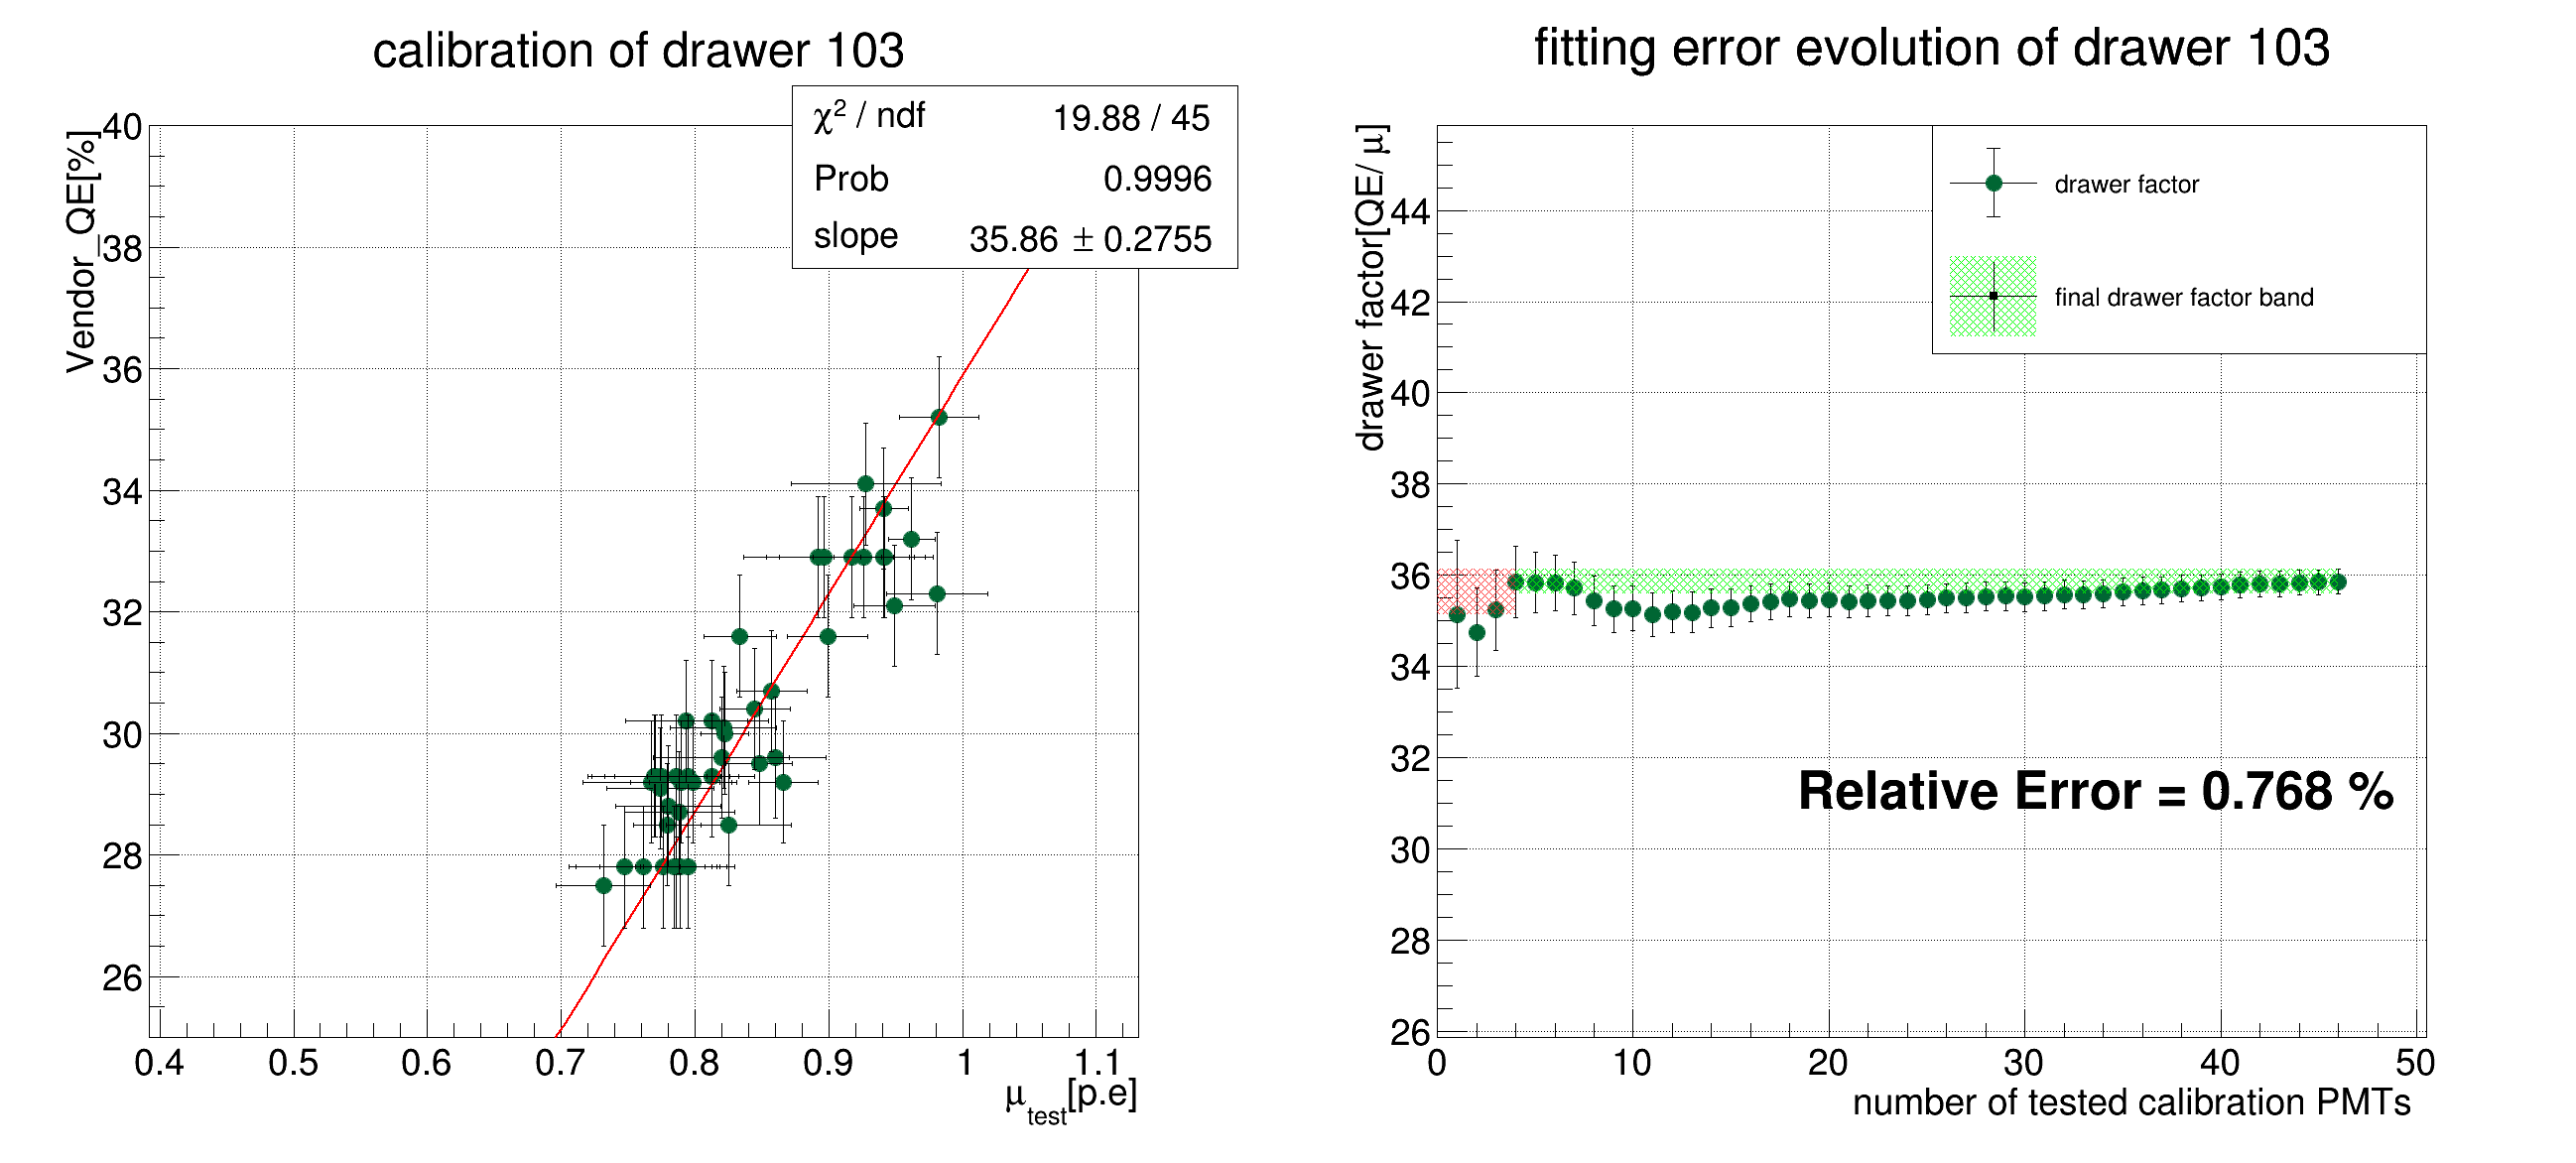
\includegraphics[width=0.45\textwidth]{sta101-2} 
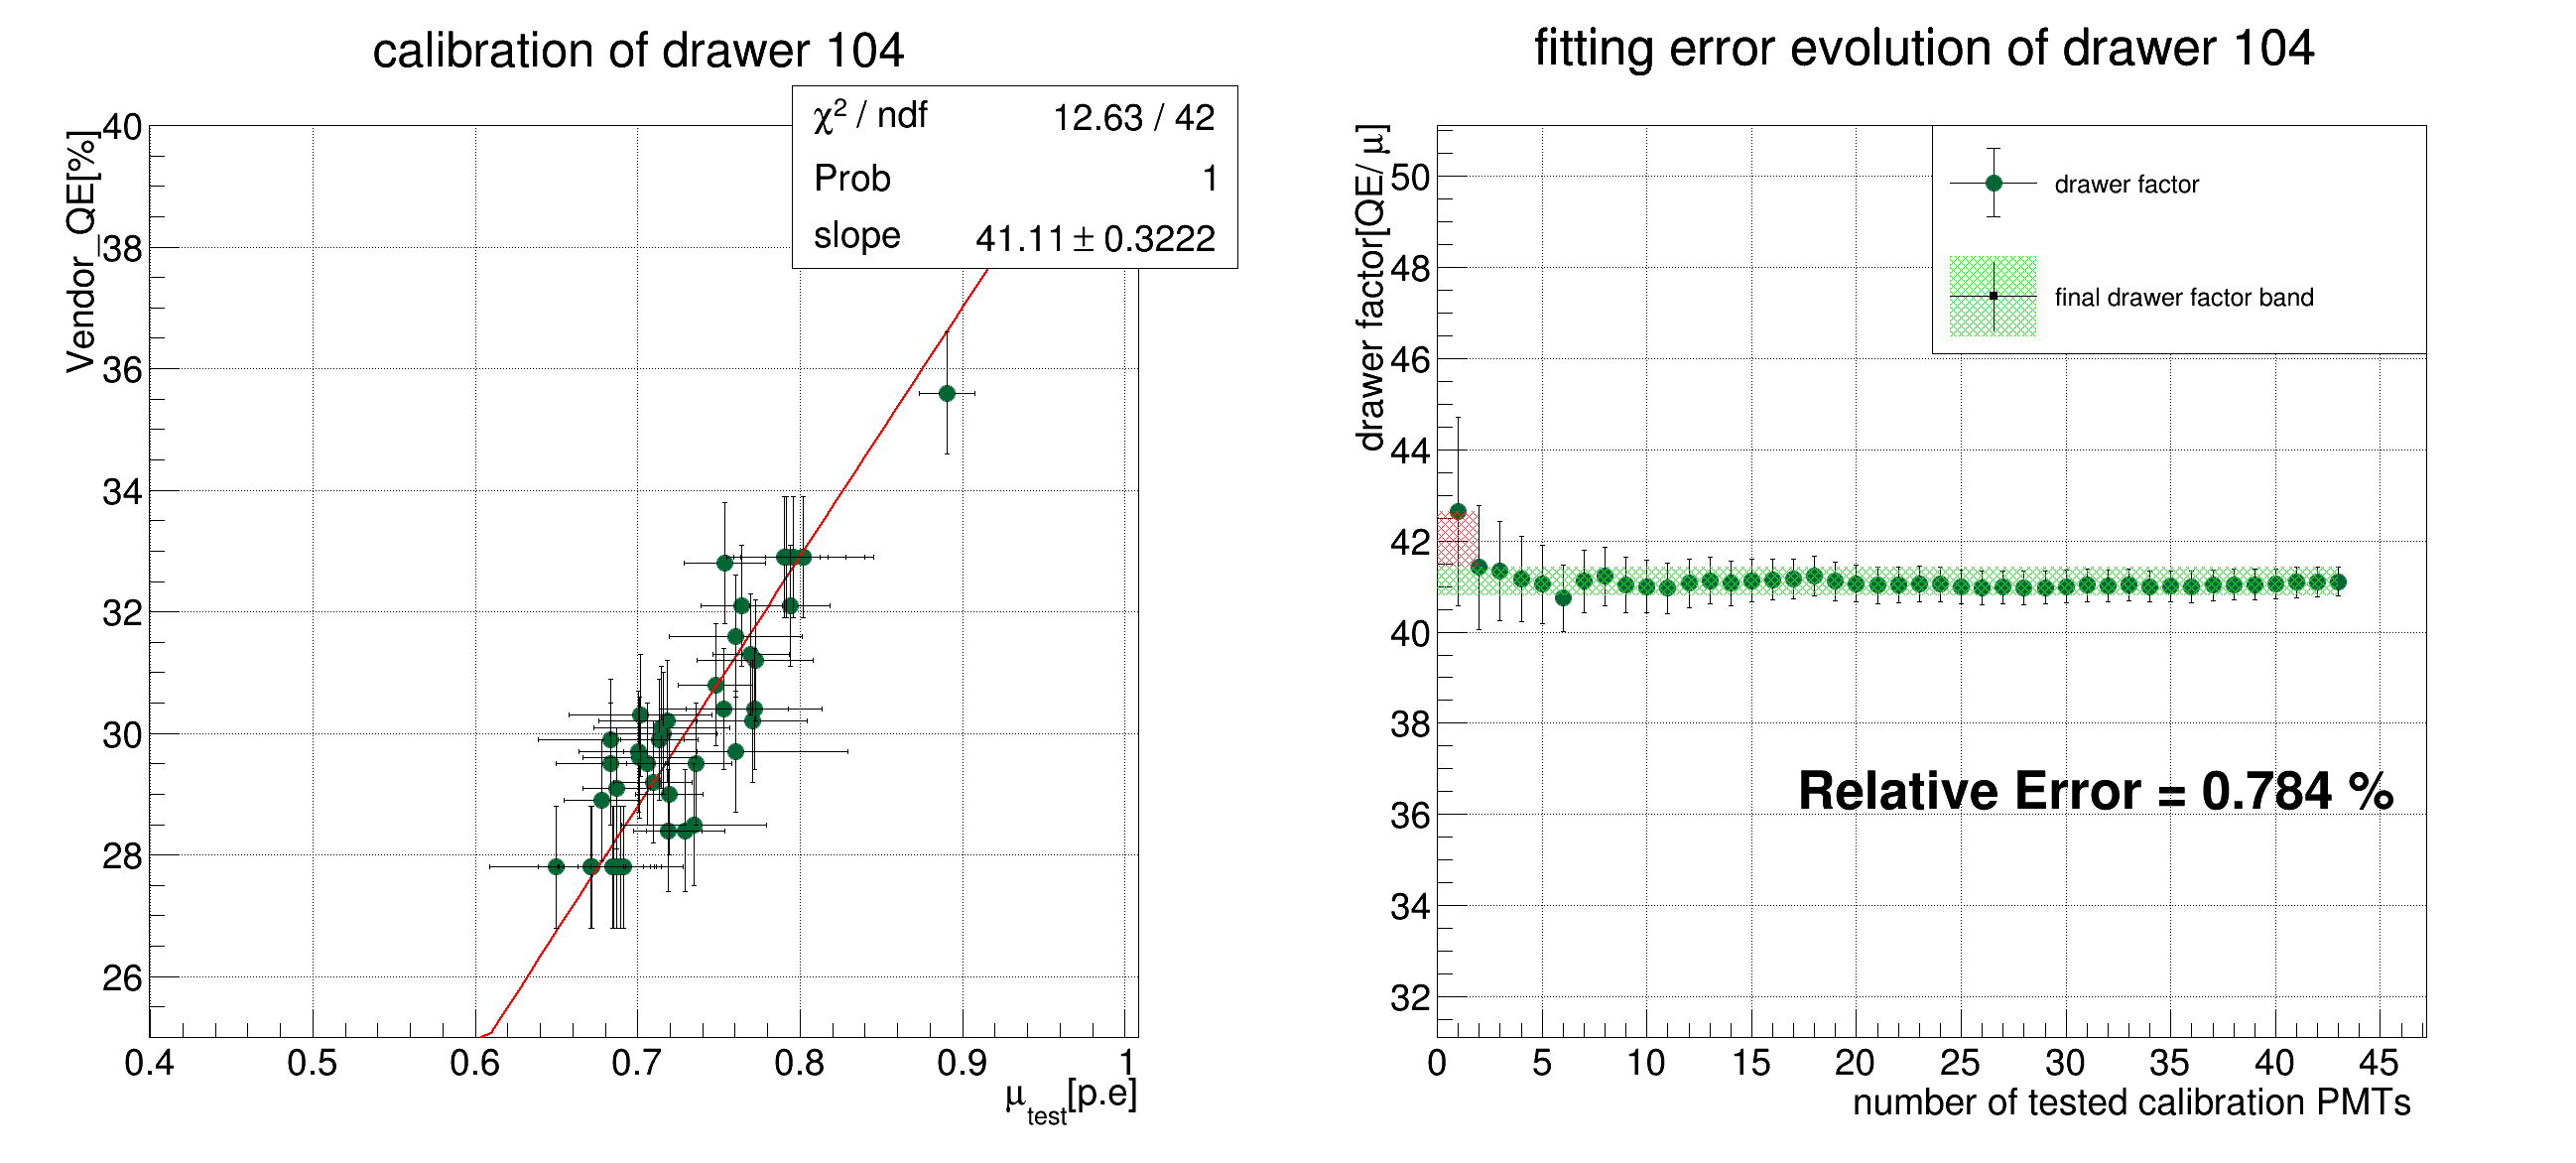
\includegraphics[width=0.45\textwidth]{sta101-3} 
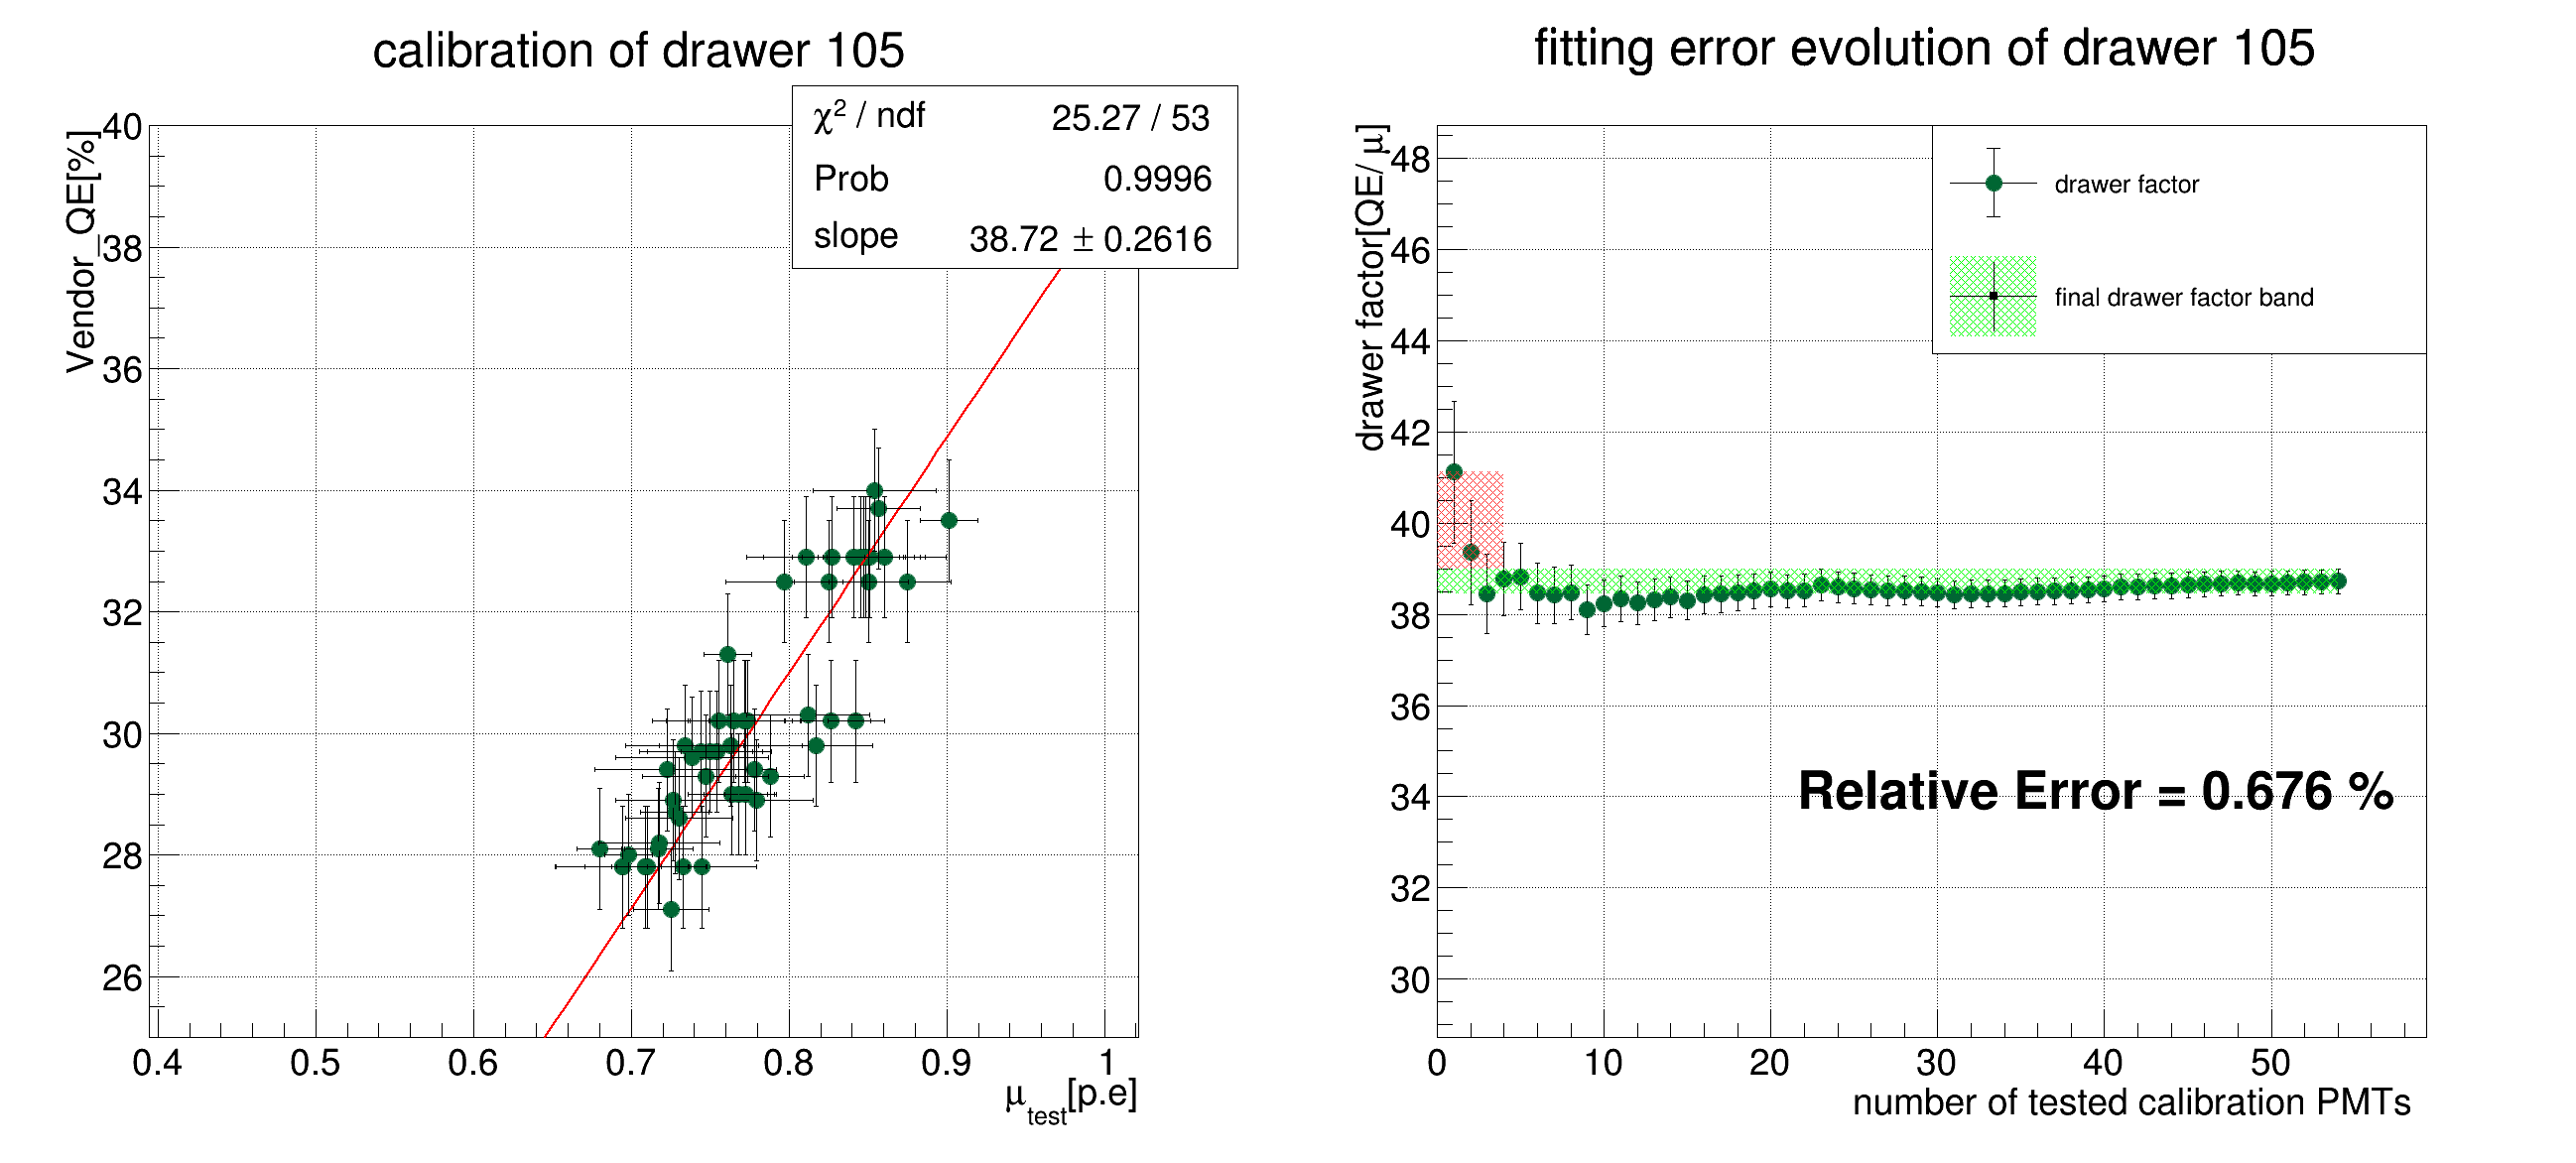
\includegraphics[width=0.45\textwidth]{sta101-4} 
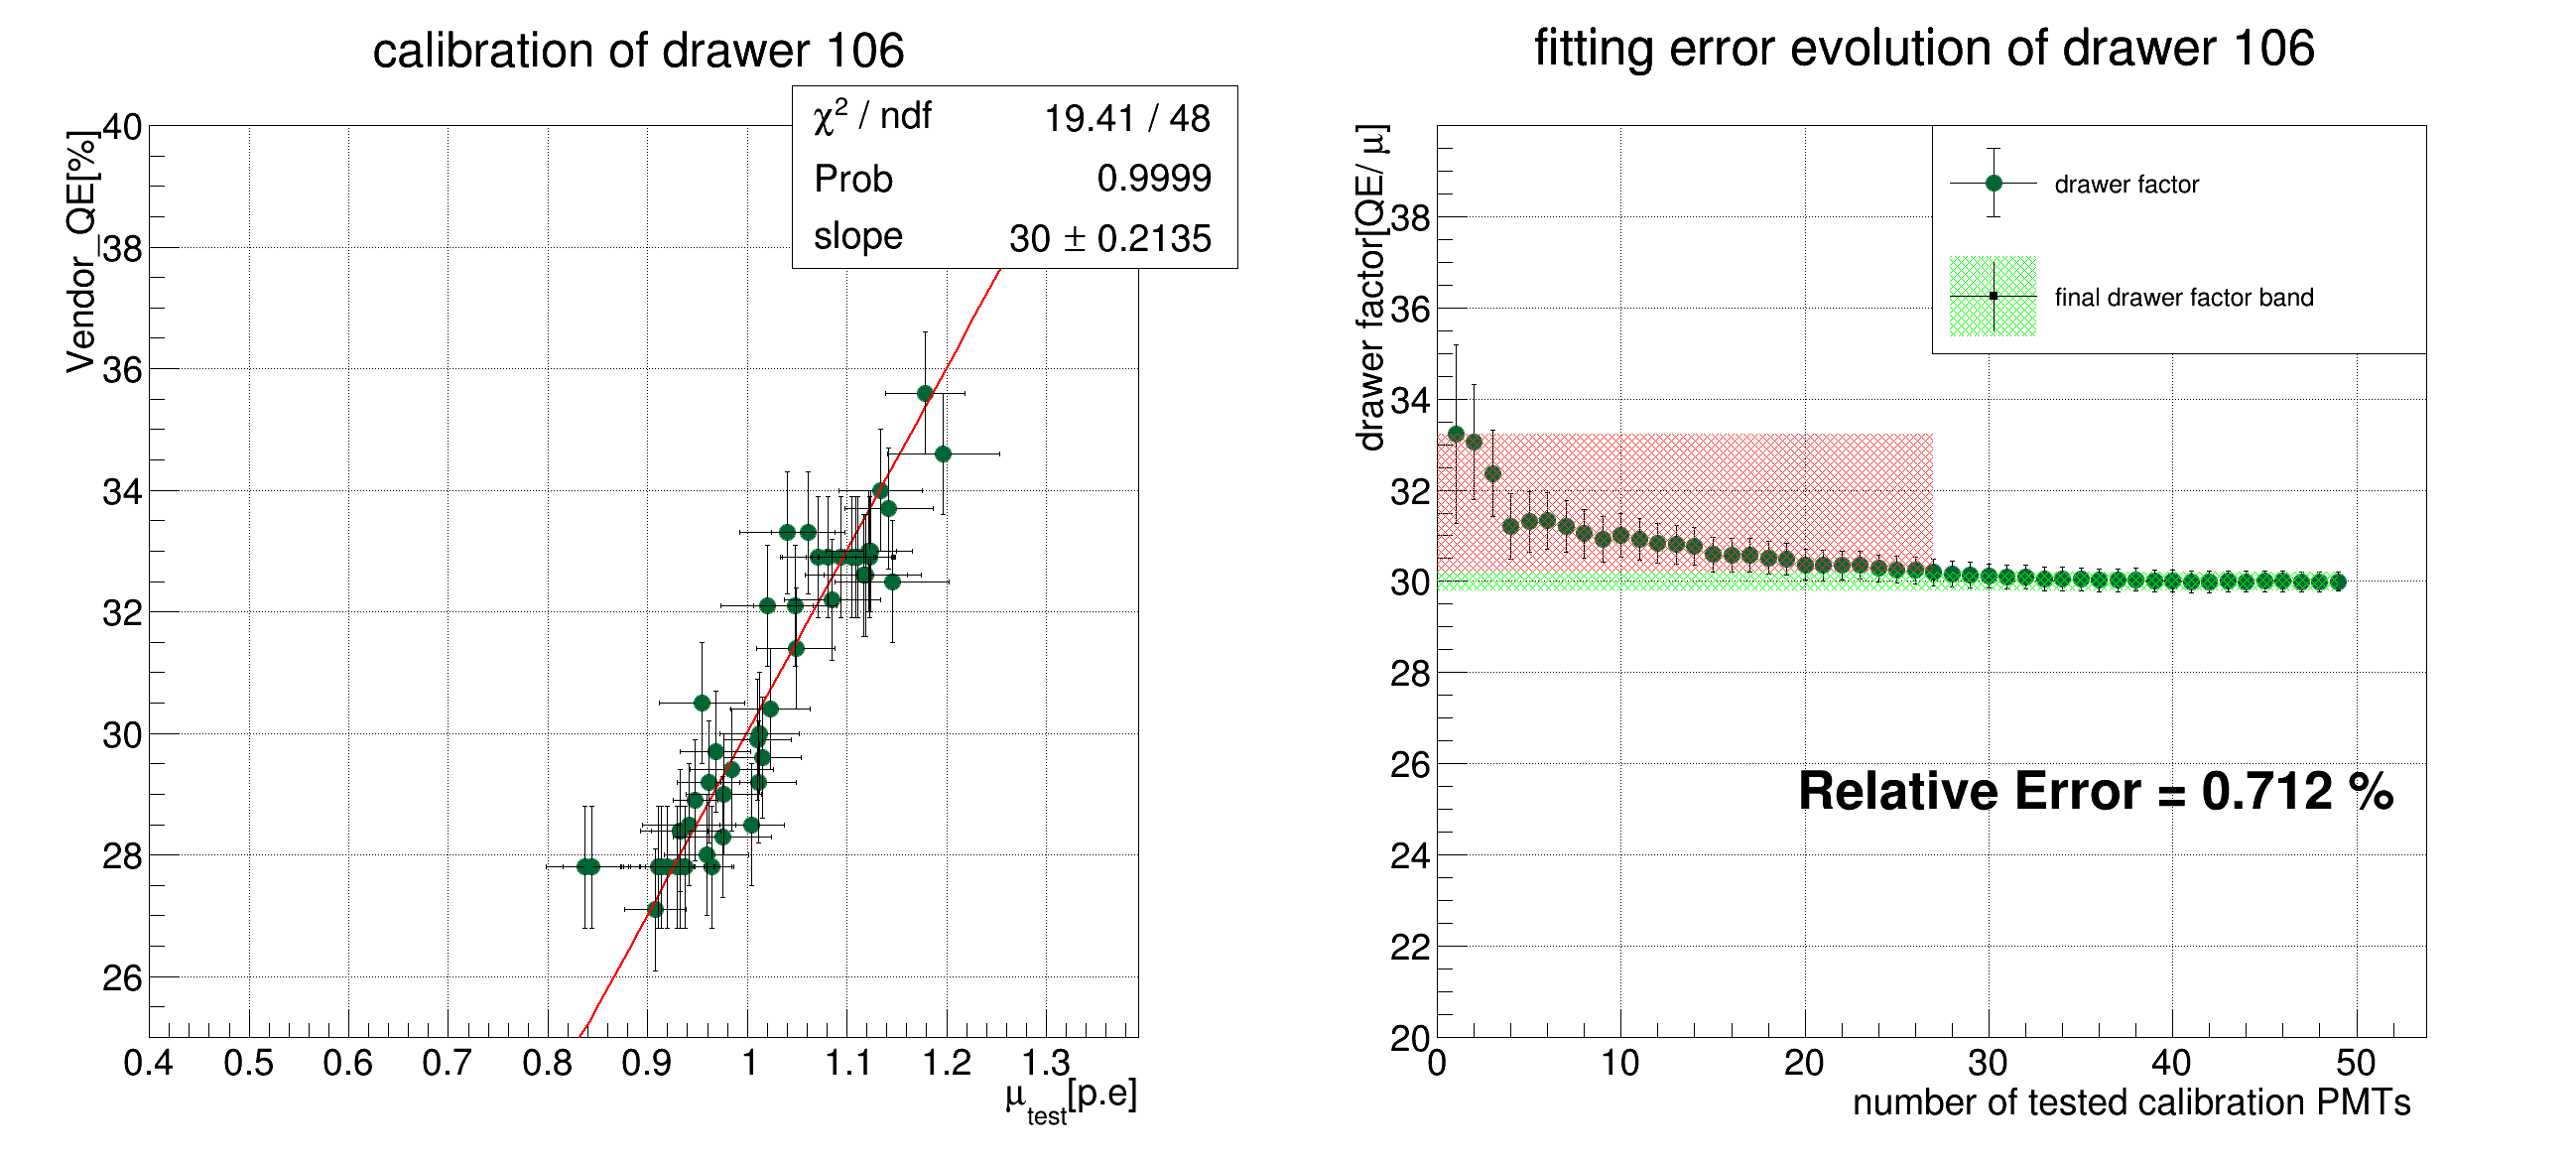
\includegraphics[width=0.45\textwidth]{sta101-5} 
\end{frame}
\begin{frame}{drawer-calibration}
\vspace{-.5cm}
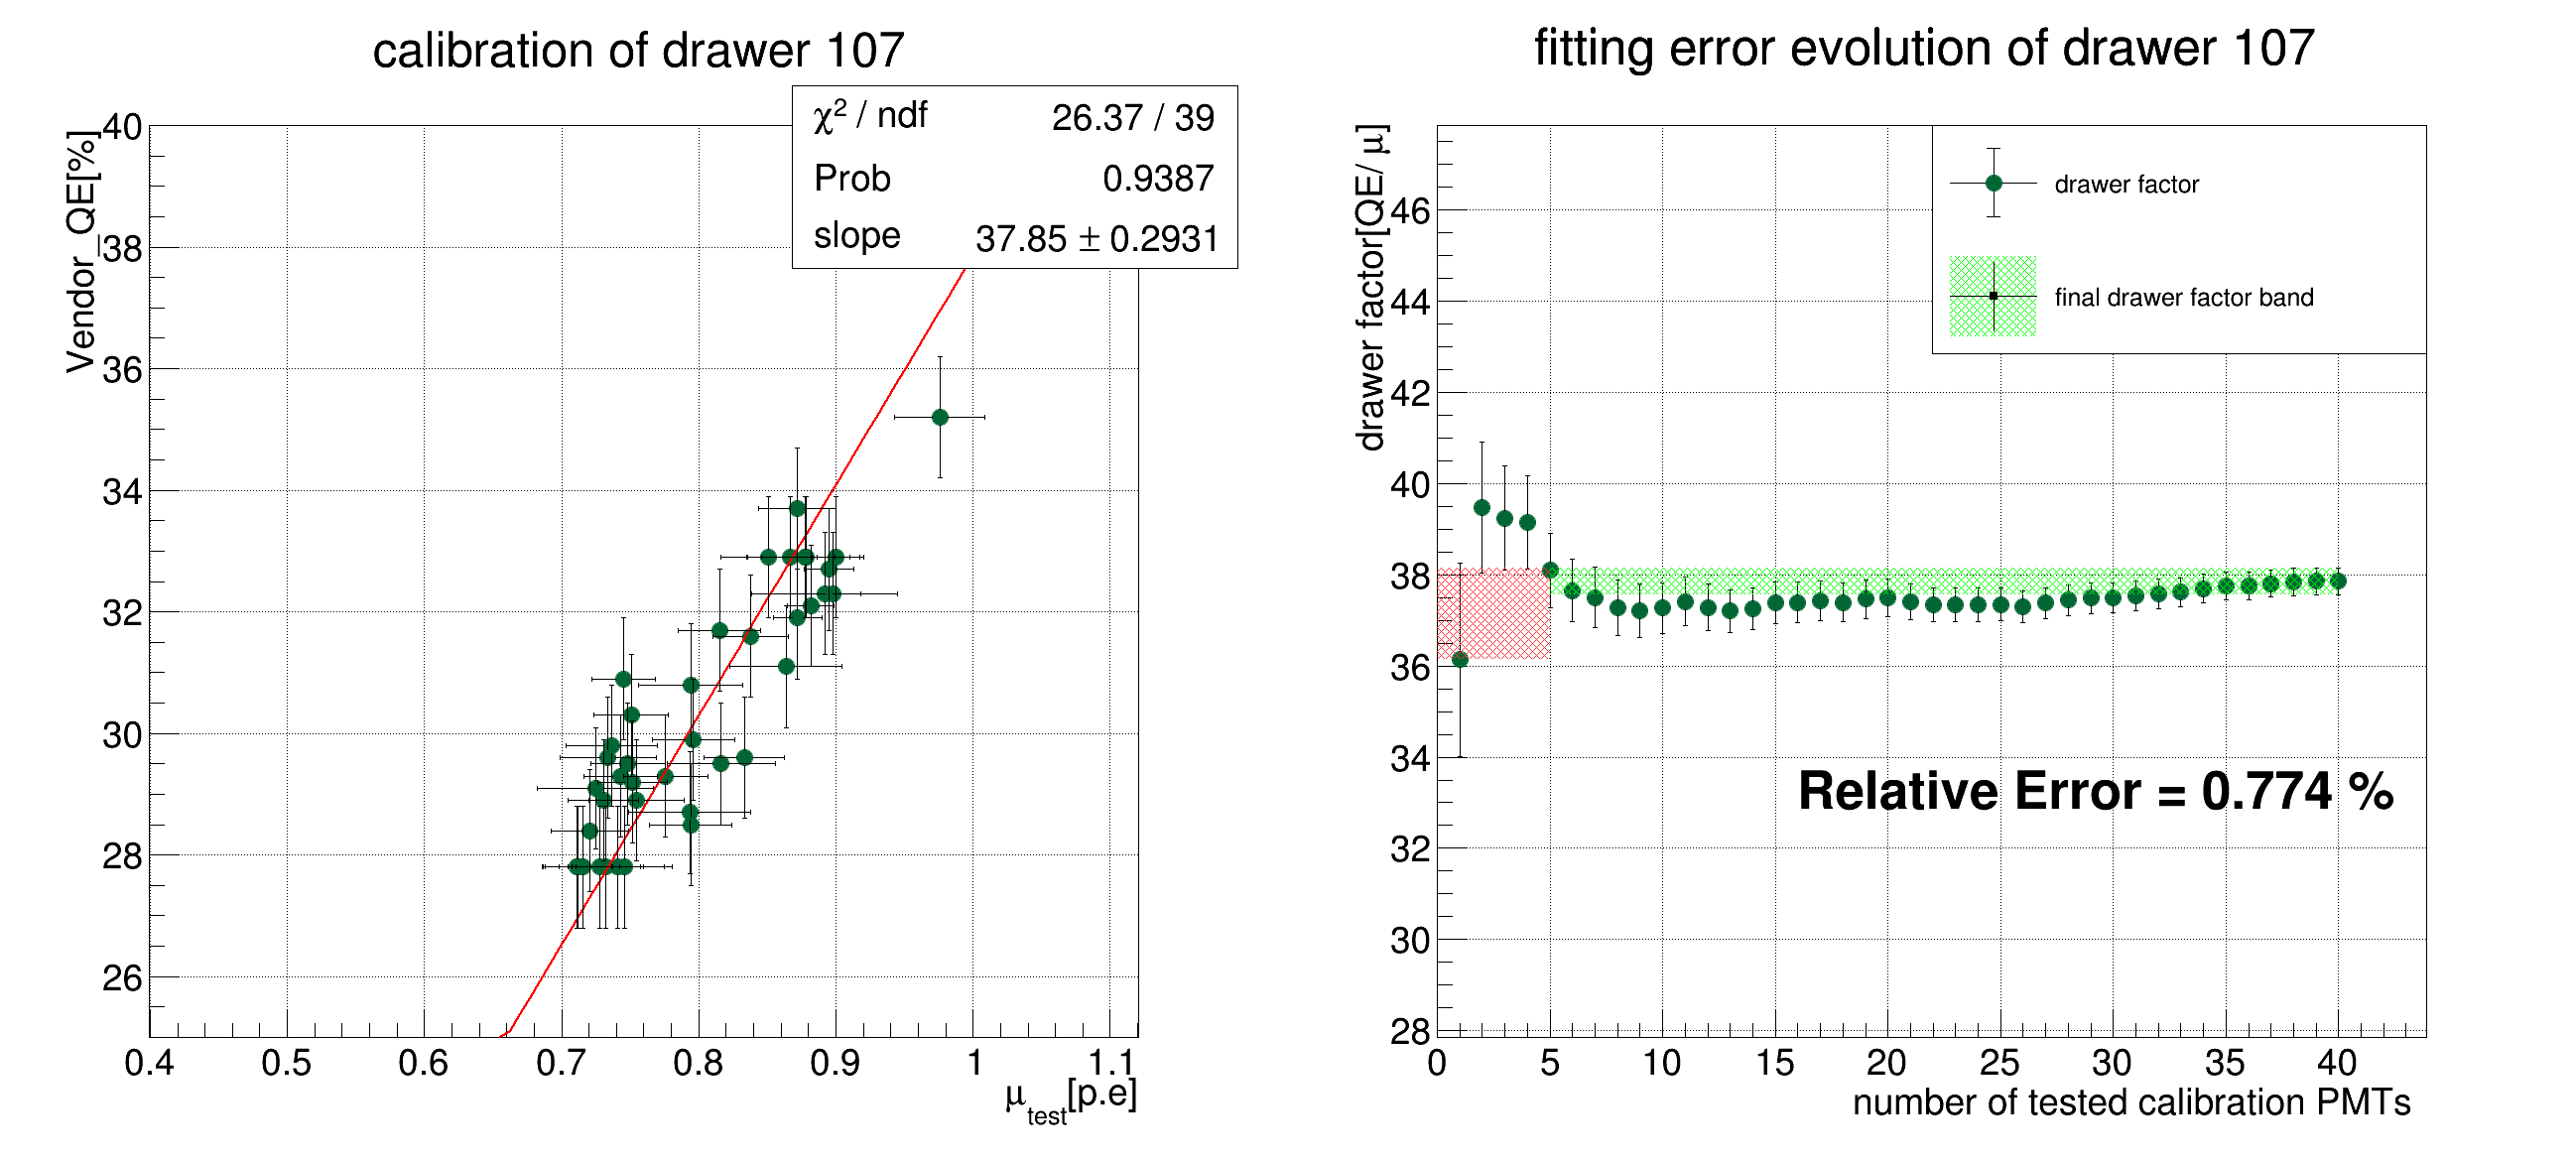
\includegraphics[width=0.45\textwidth]{sta101-6} 
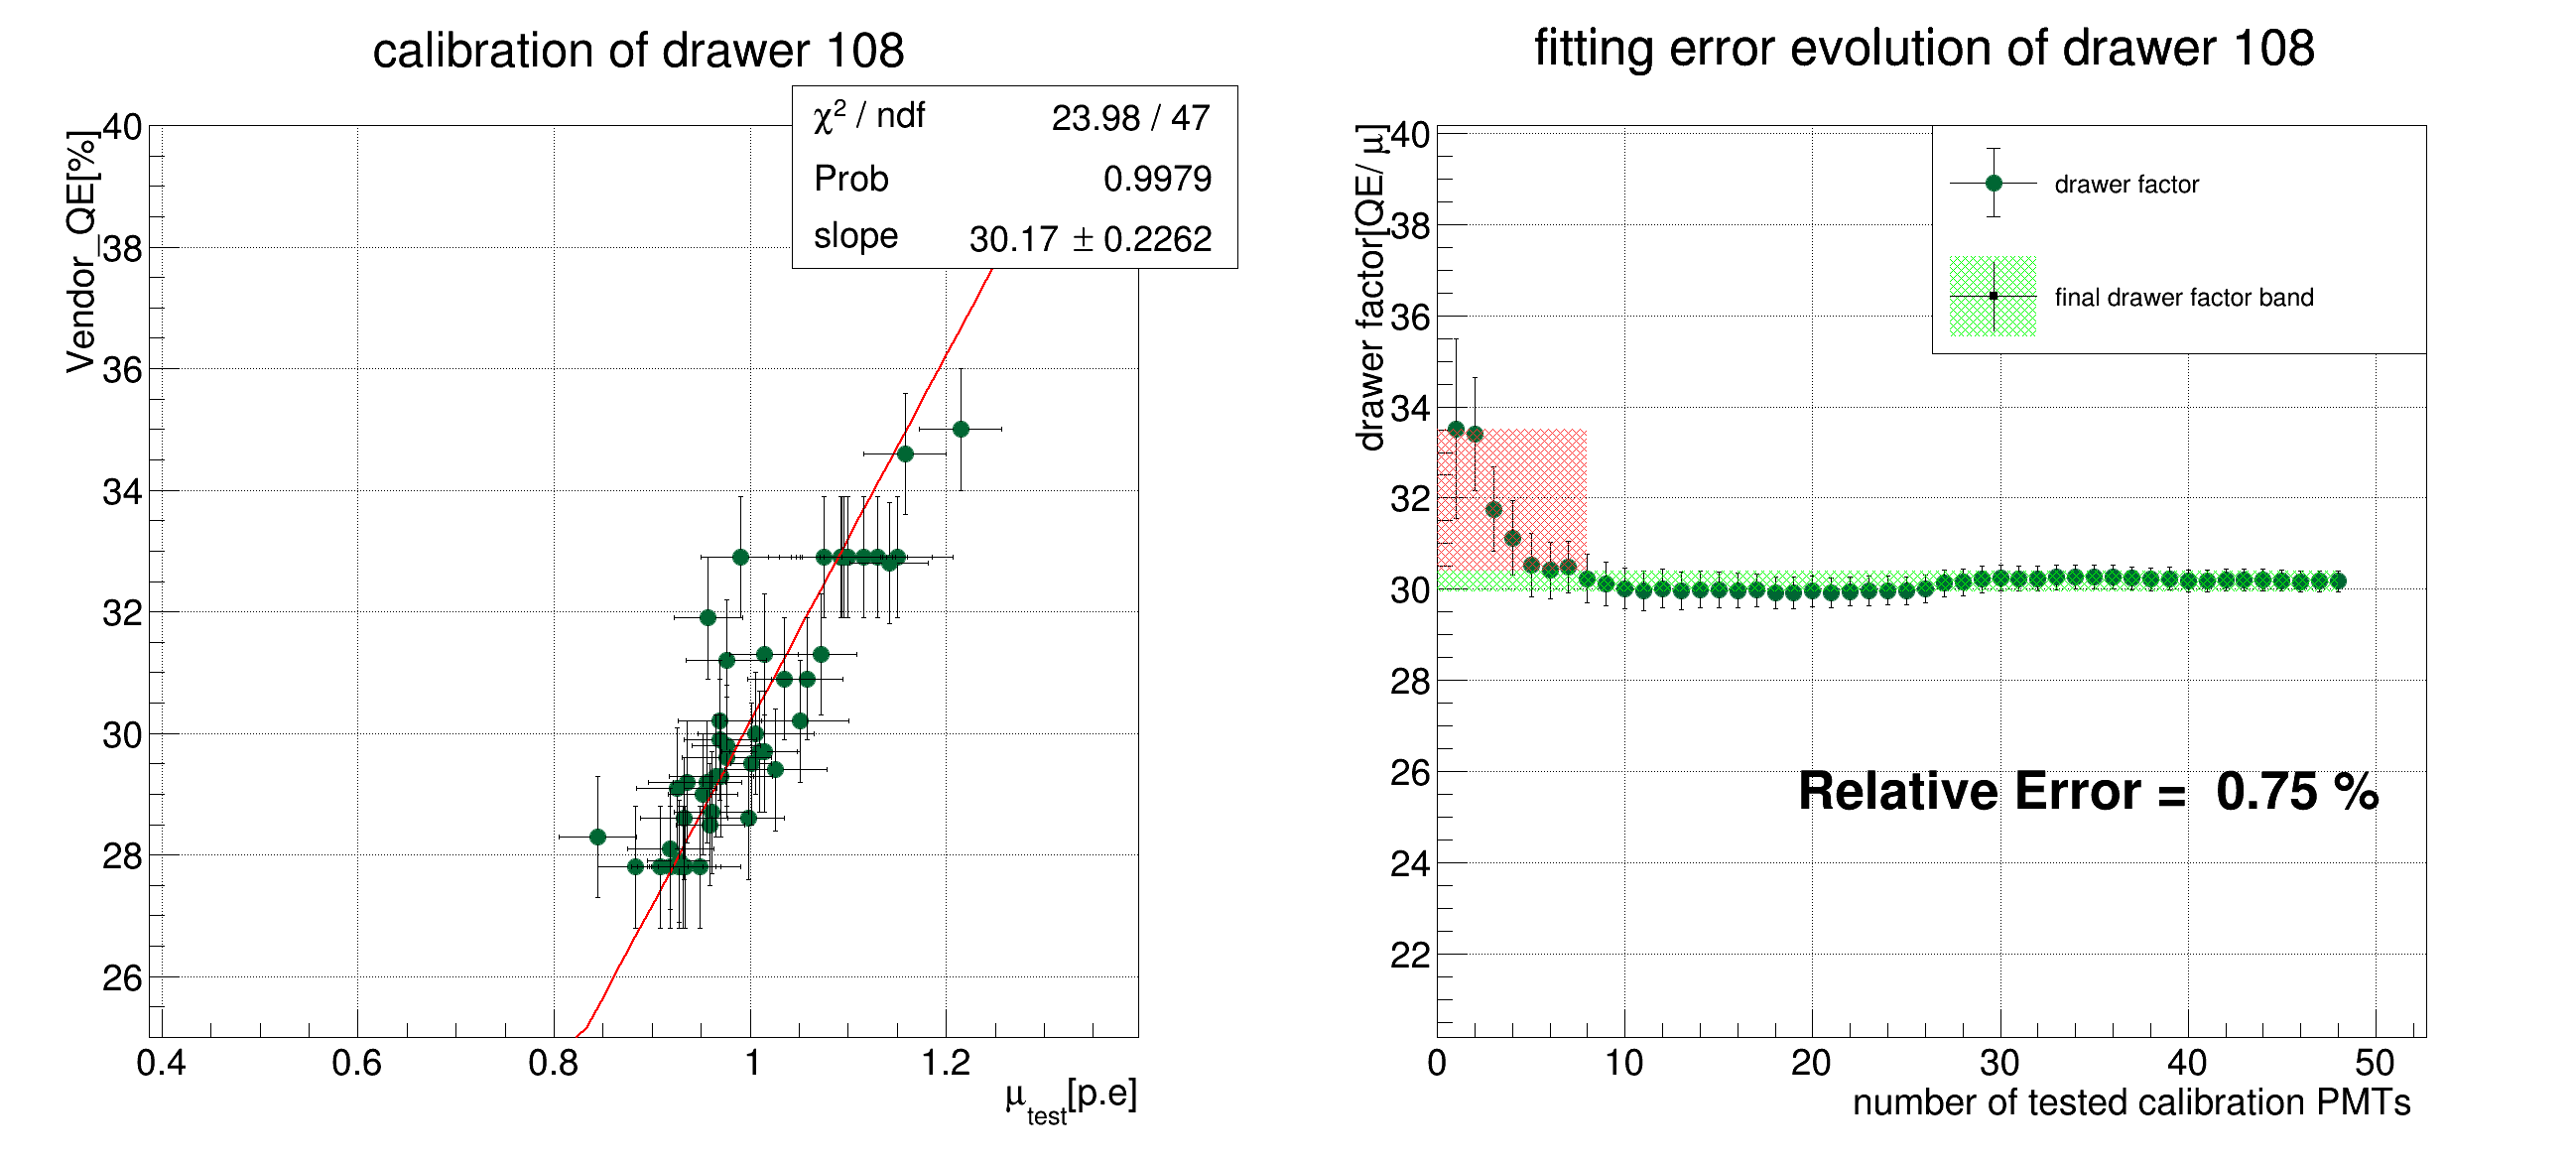
\includegraphics[width=0.45\textwidth]{sta101-7} 
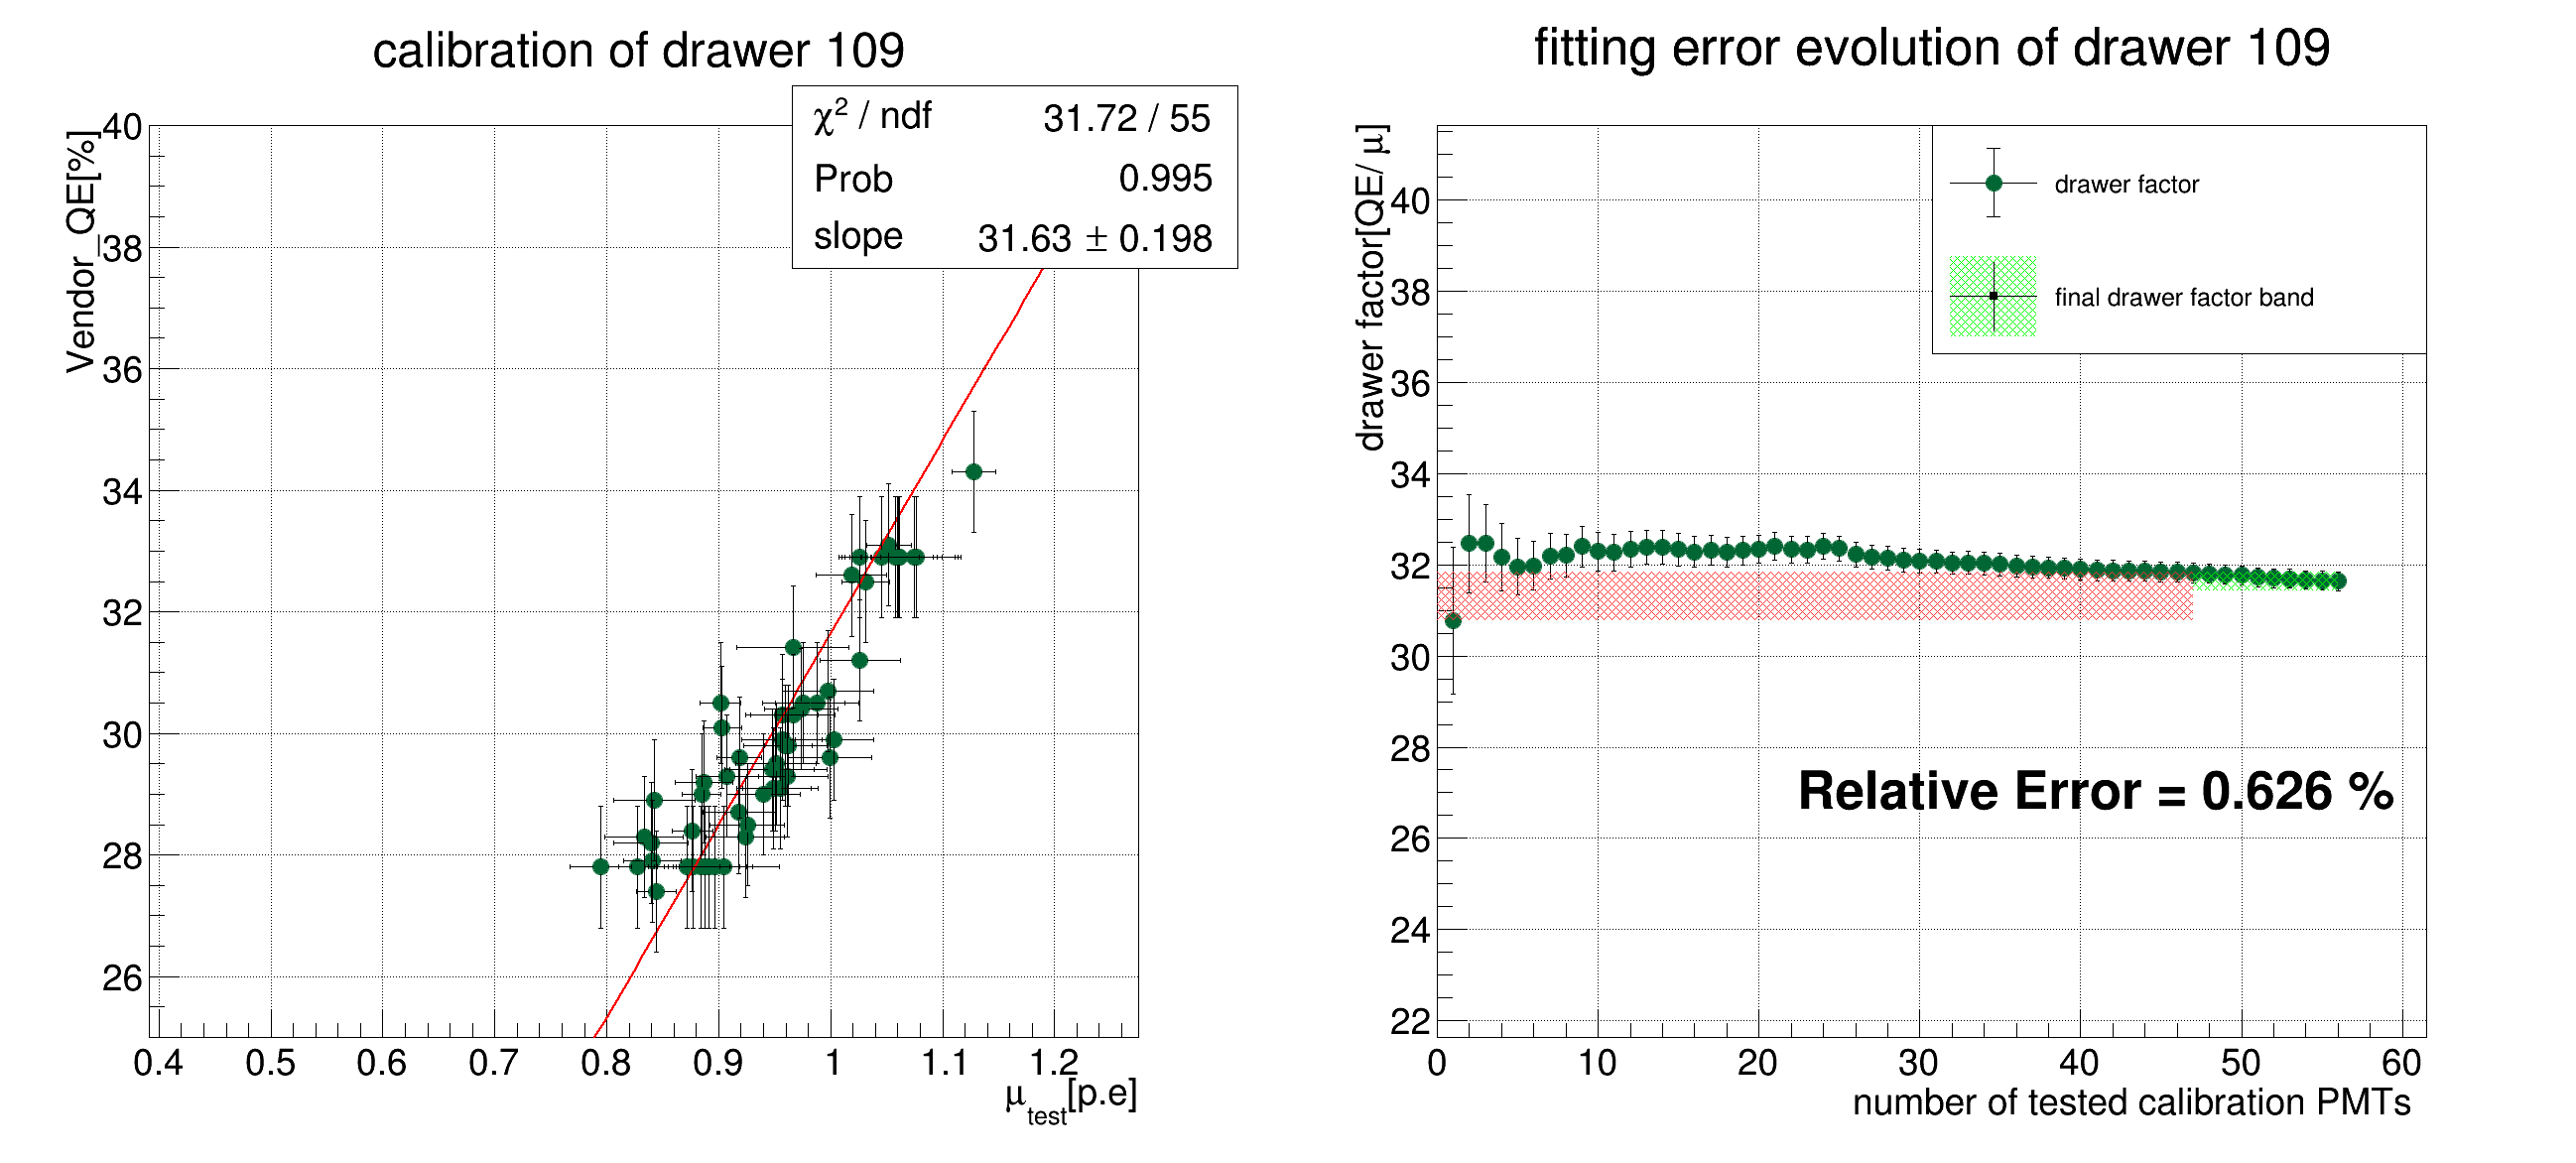
\includegraphics[width=0.45\textwidth]{sta101-8} 
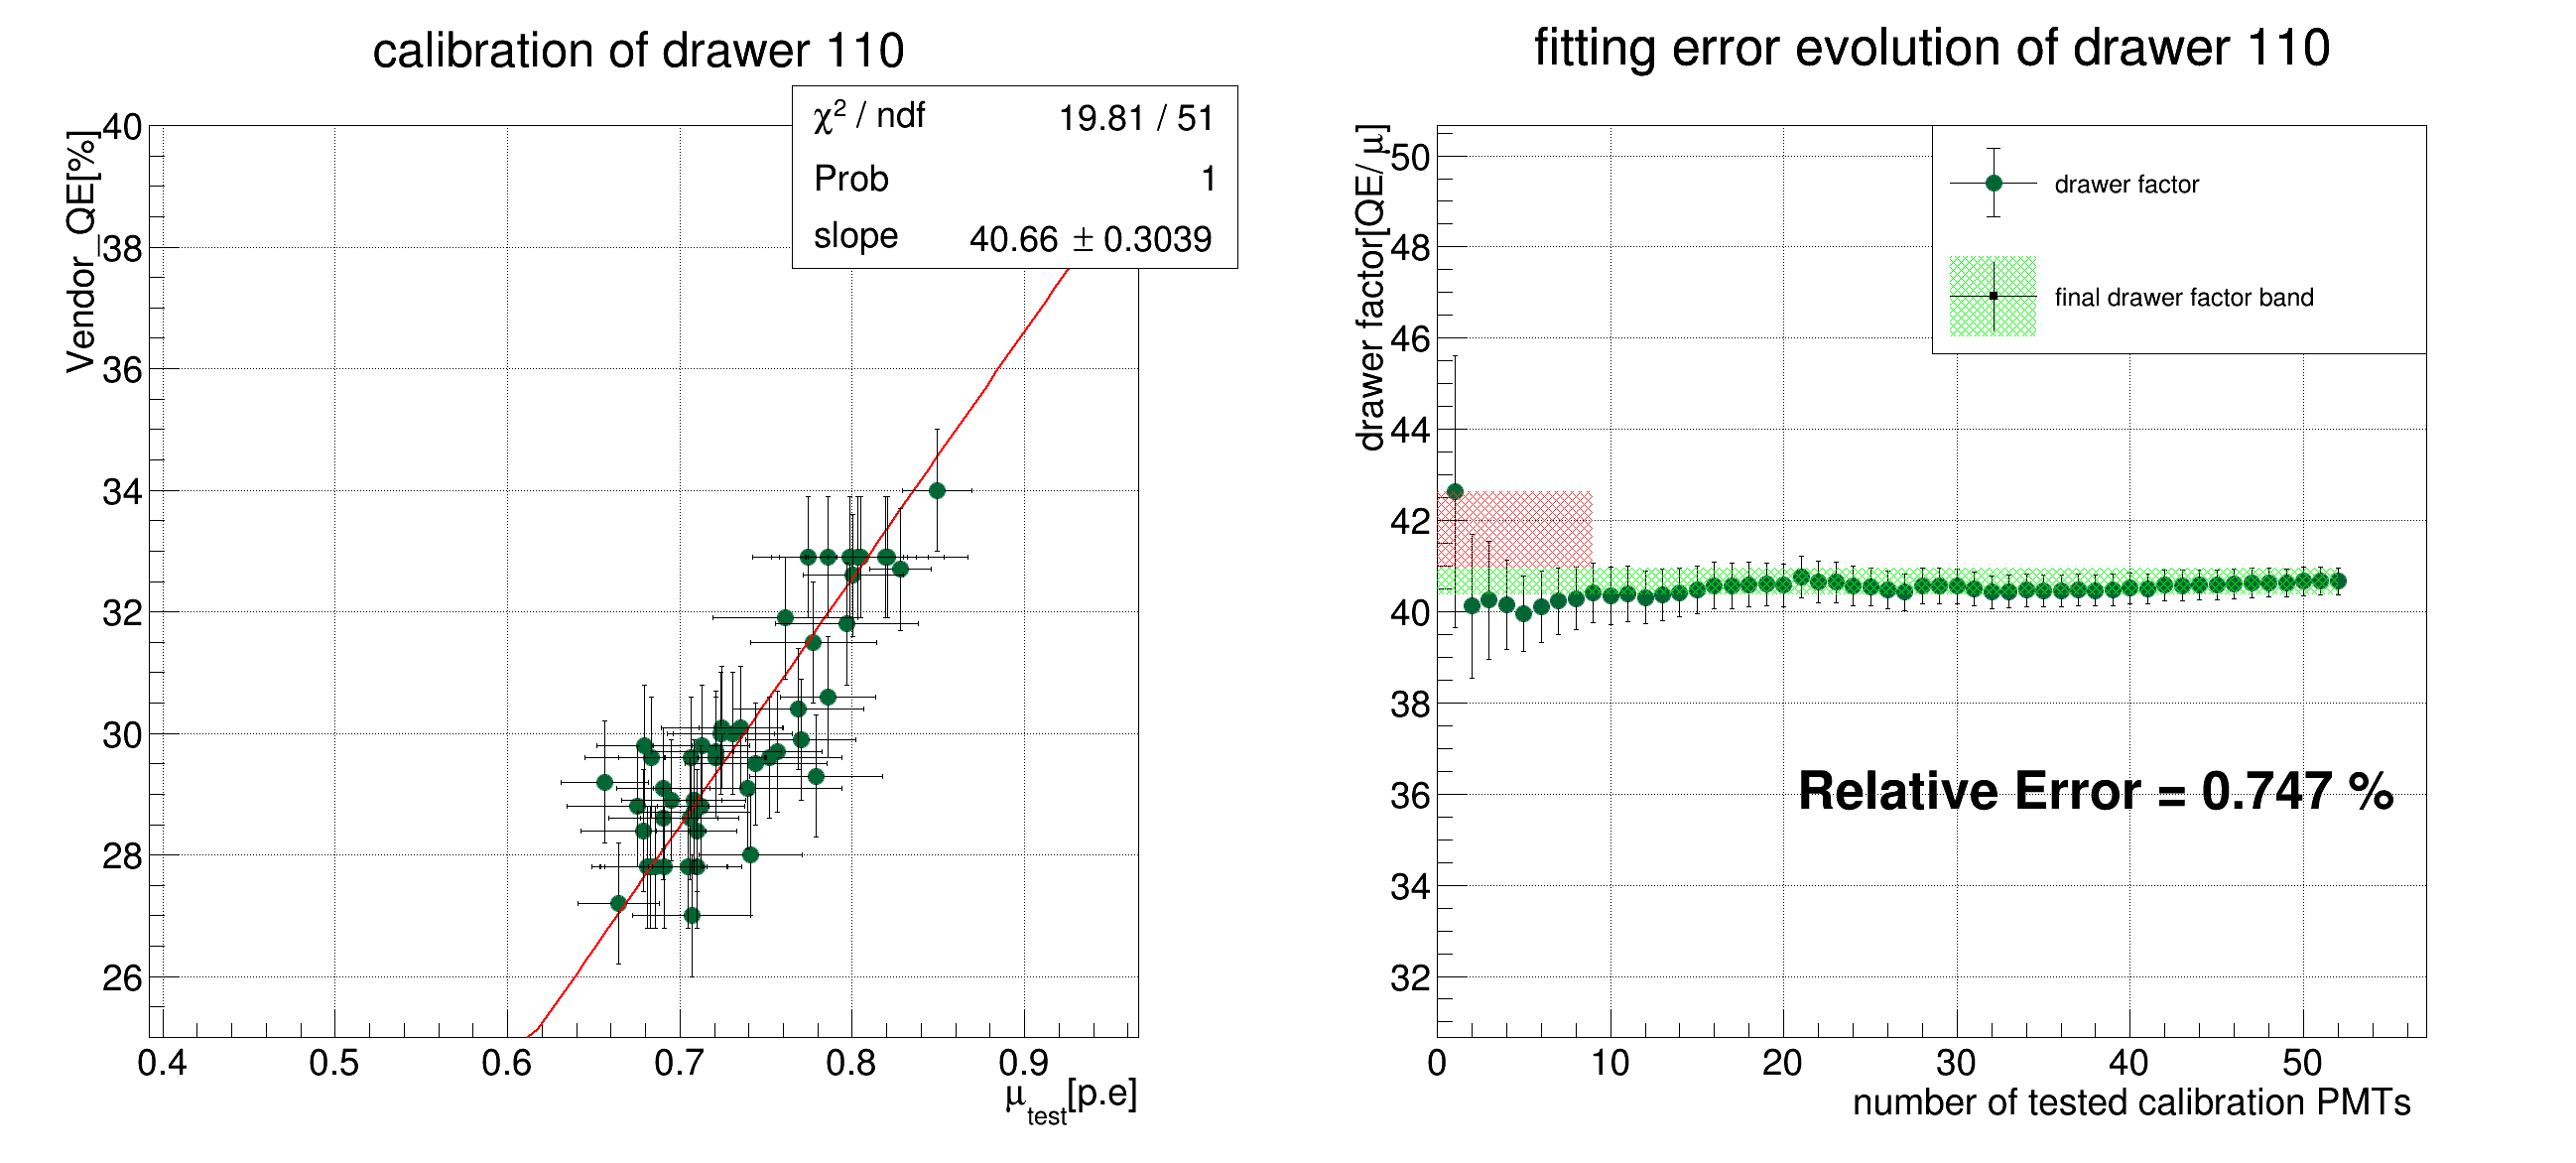
\includegraphics[width=0.45\textwidth]{sta101-9} 
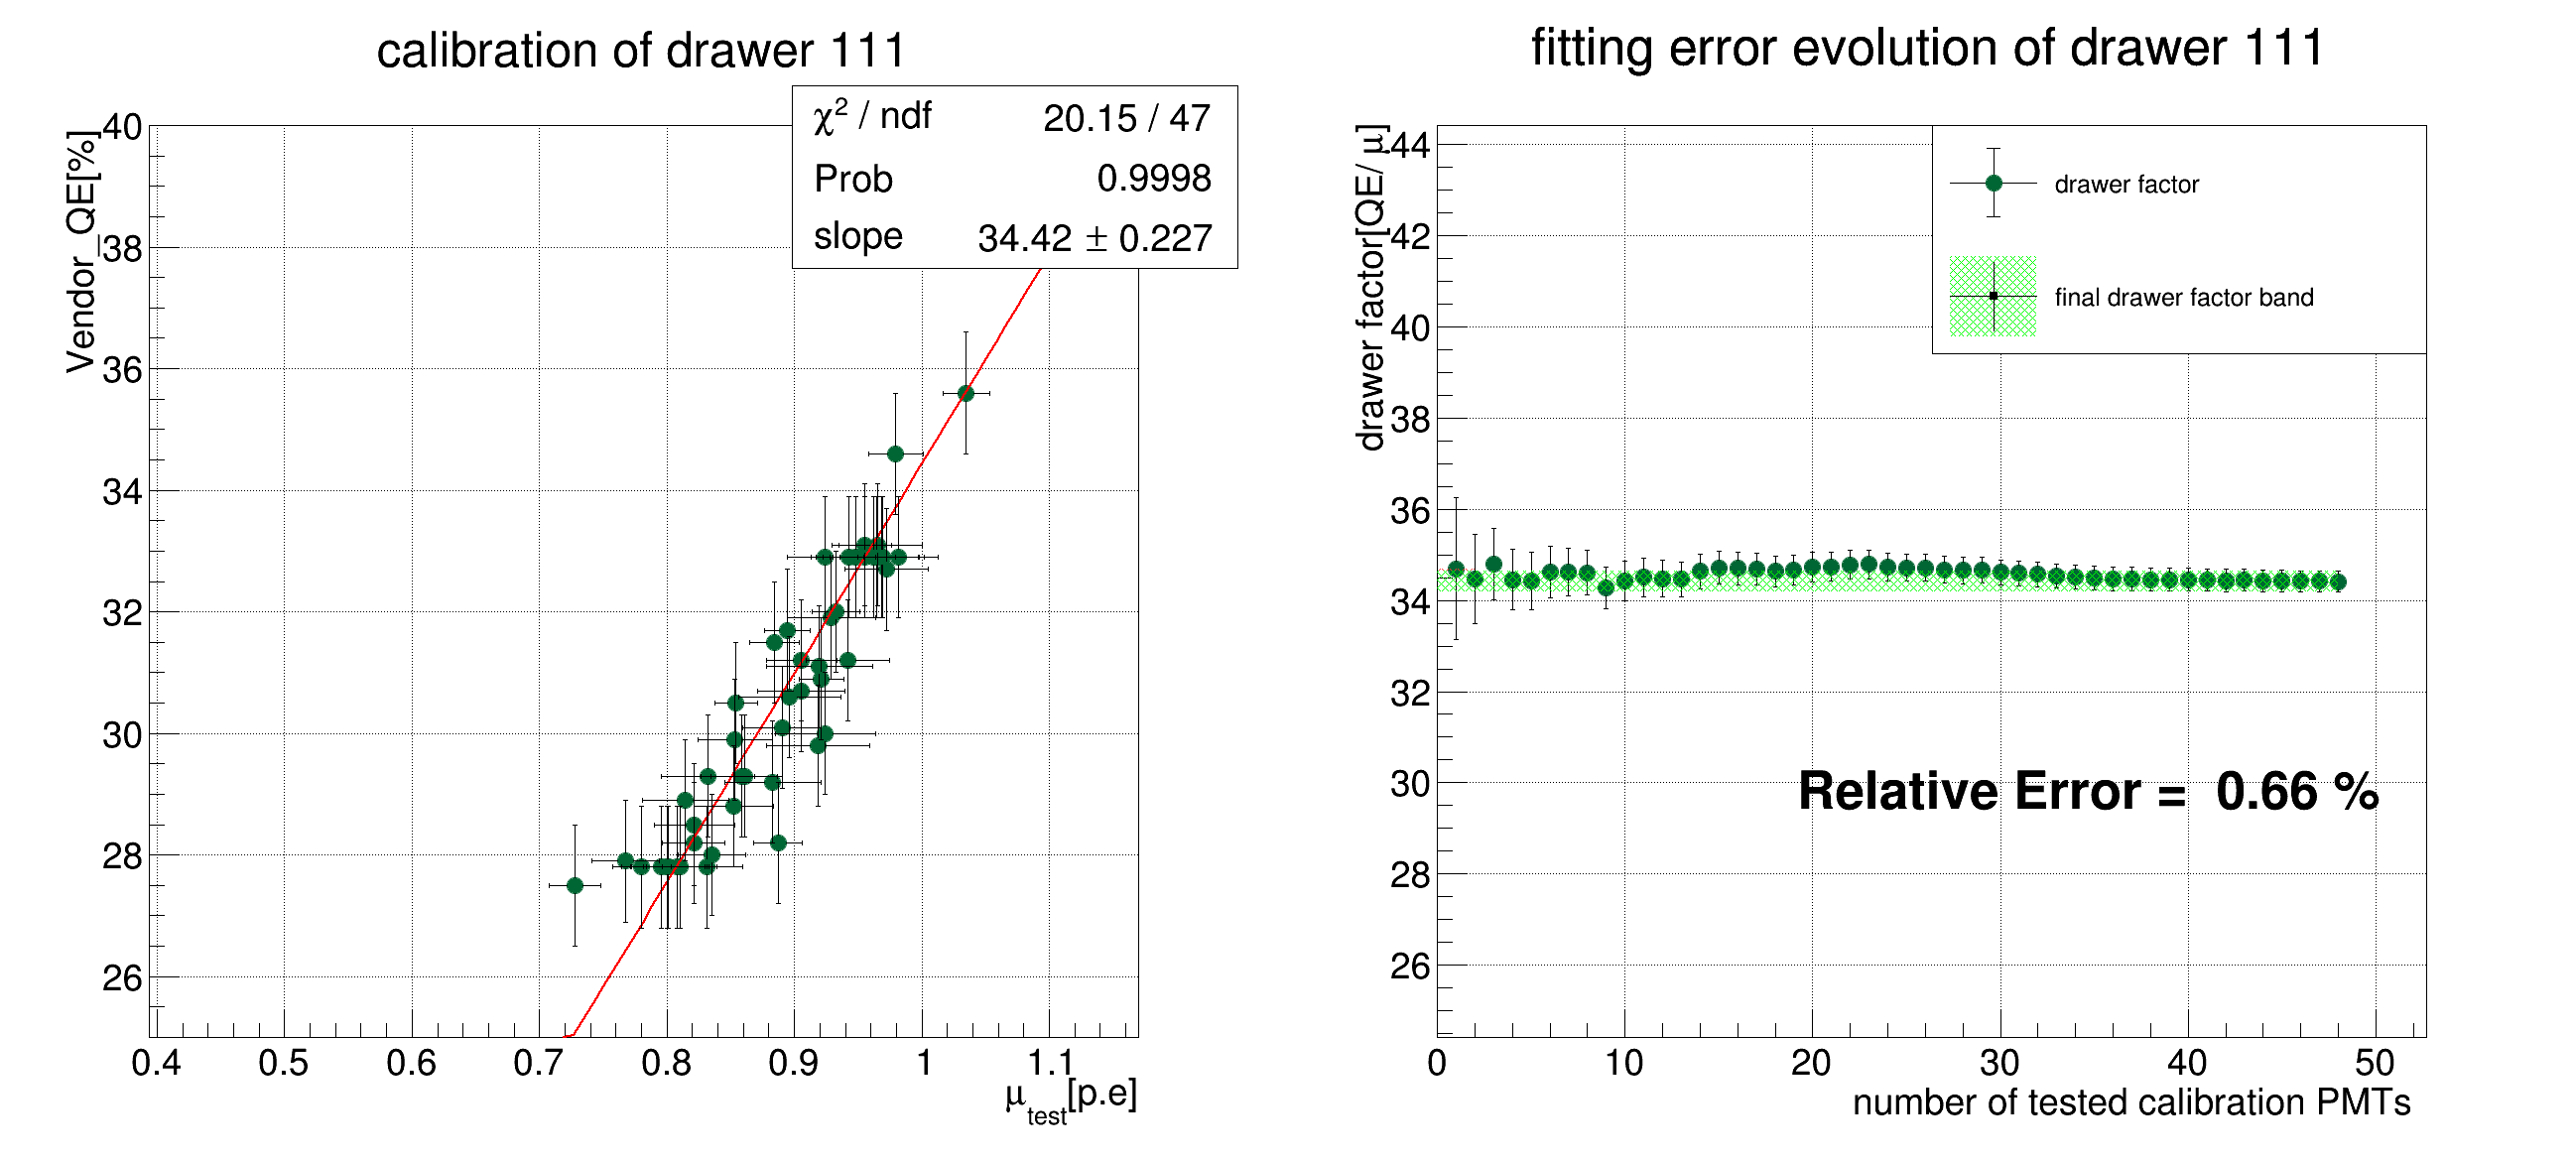
\includegraphics[width=0.45\textwidth]{sta101-10} 
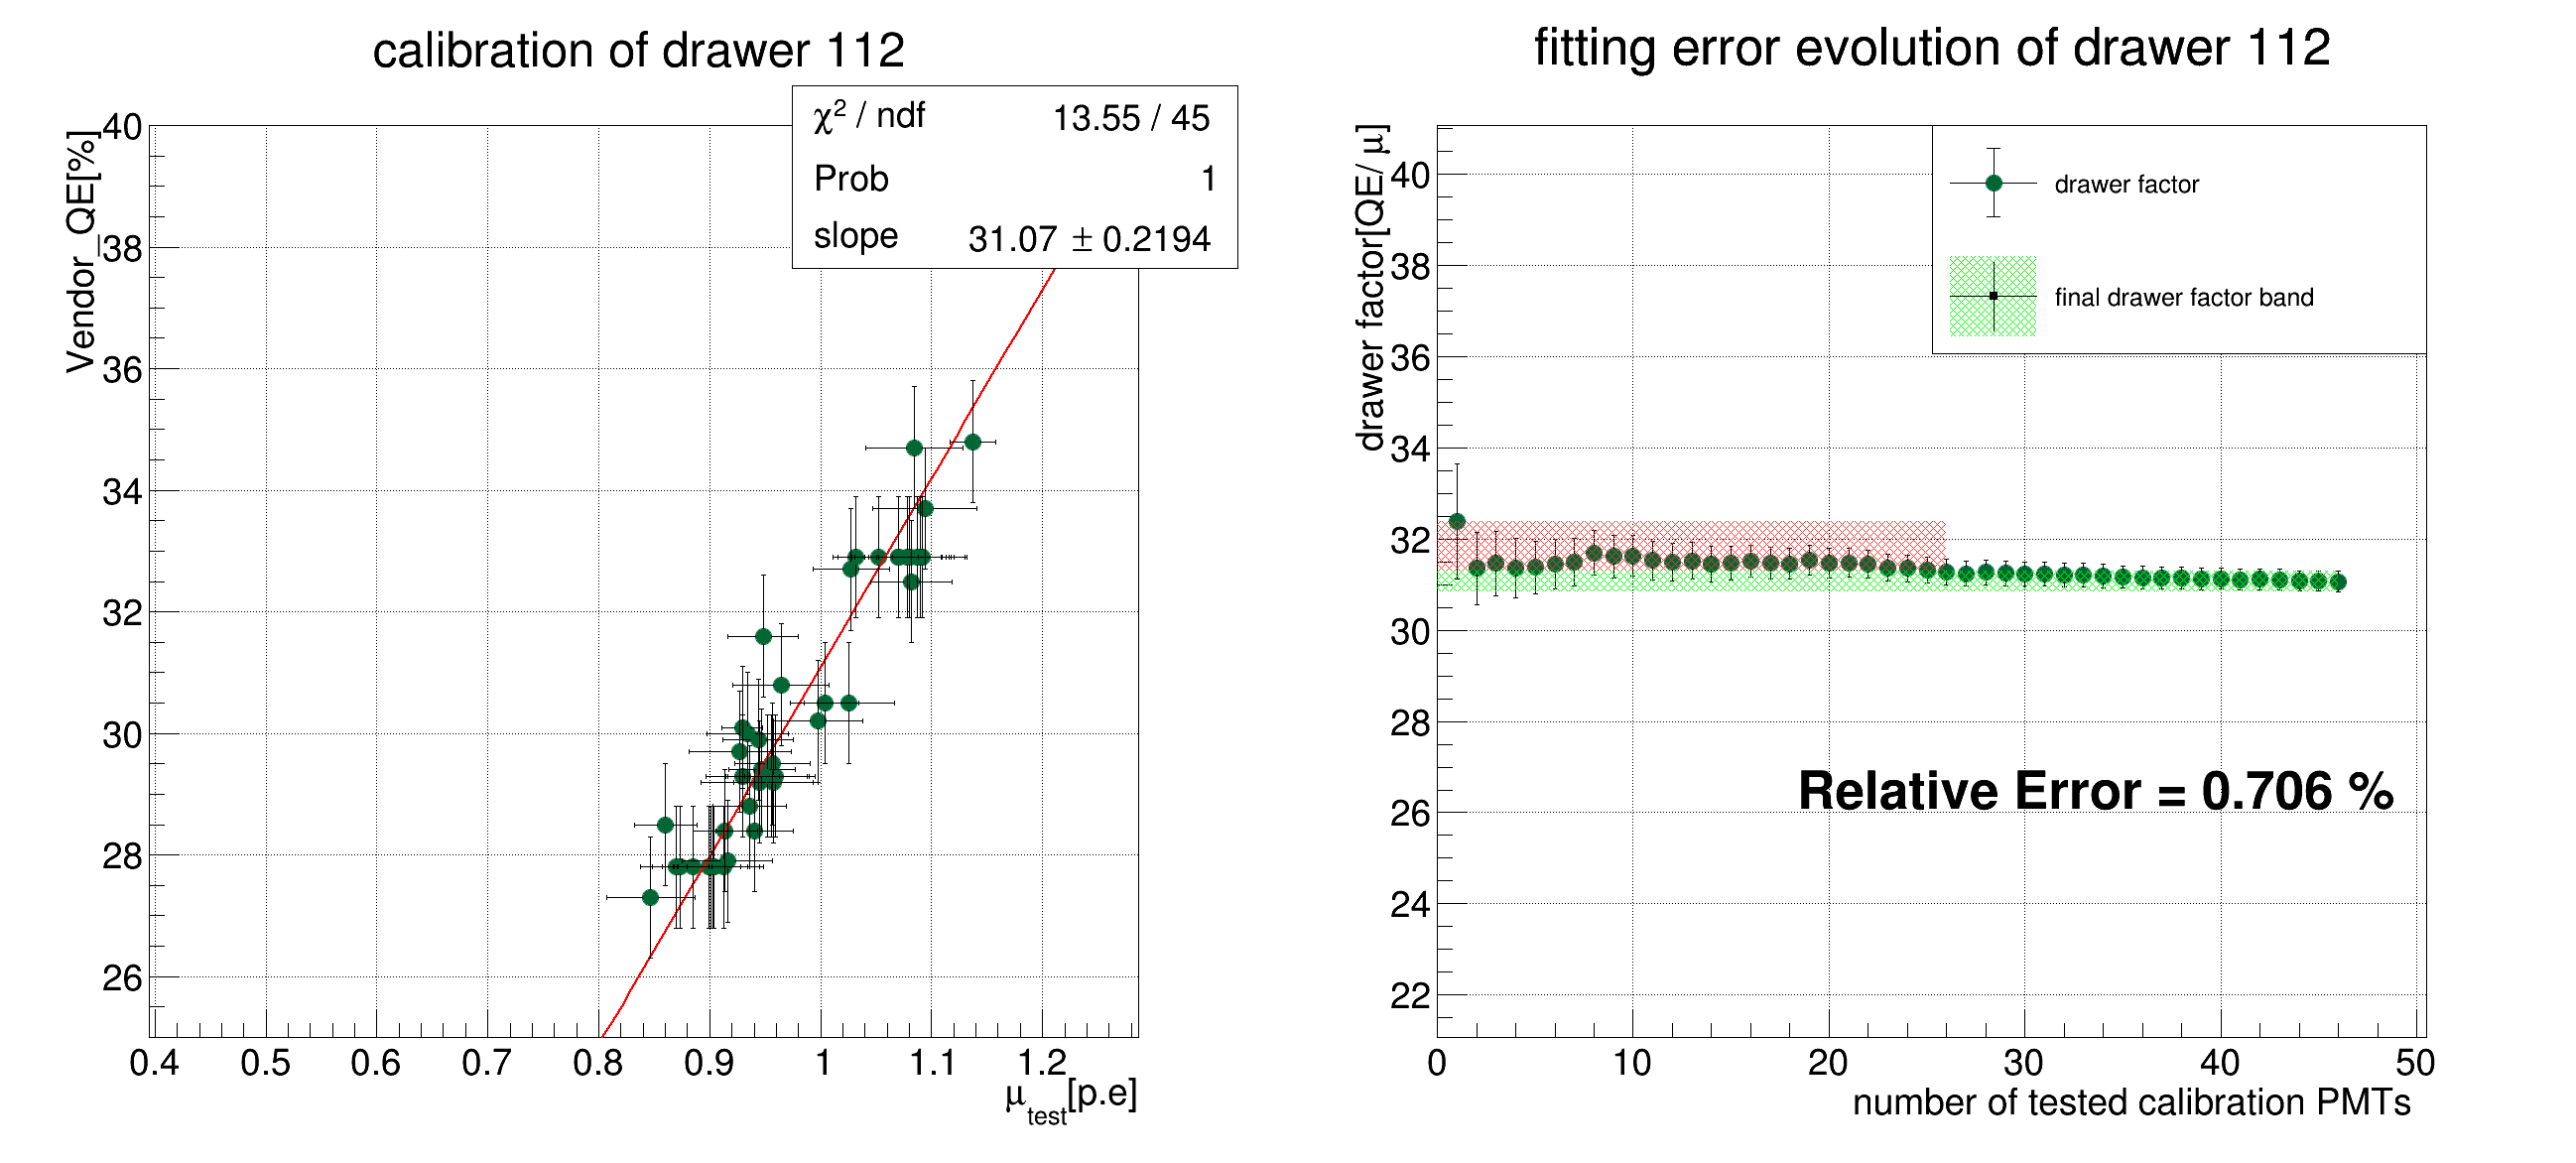
\includegraphics[width=0.45\textwidth]{sta101-11} 
\end{frame}
\begin{frame}{drawer-calibration}
\vspace{-.5cm}
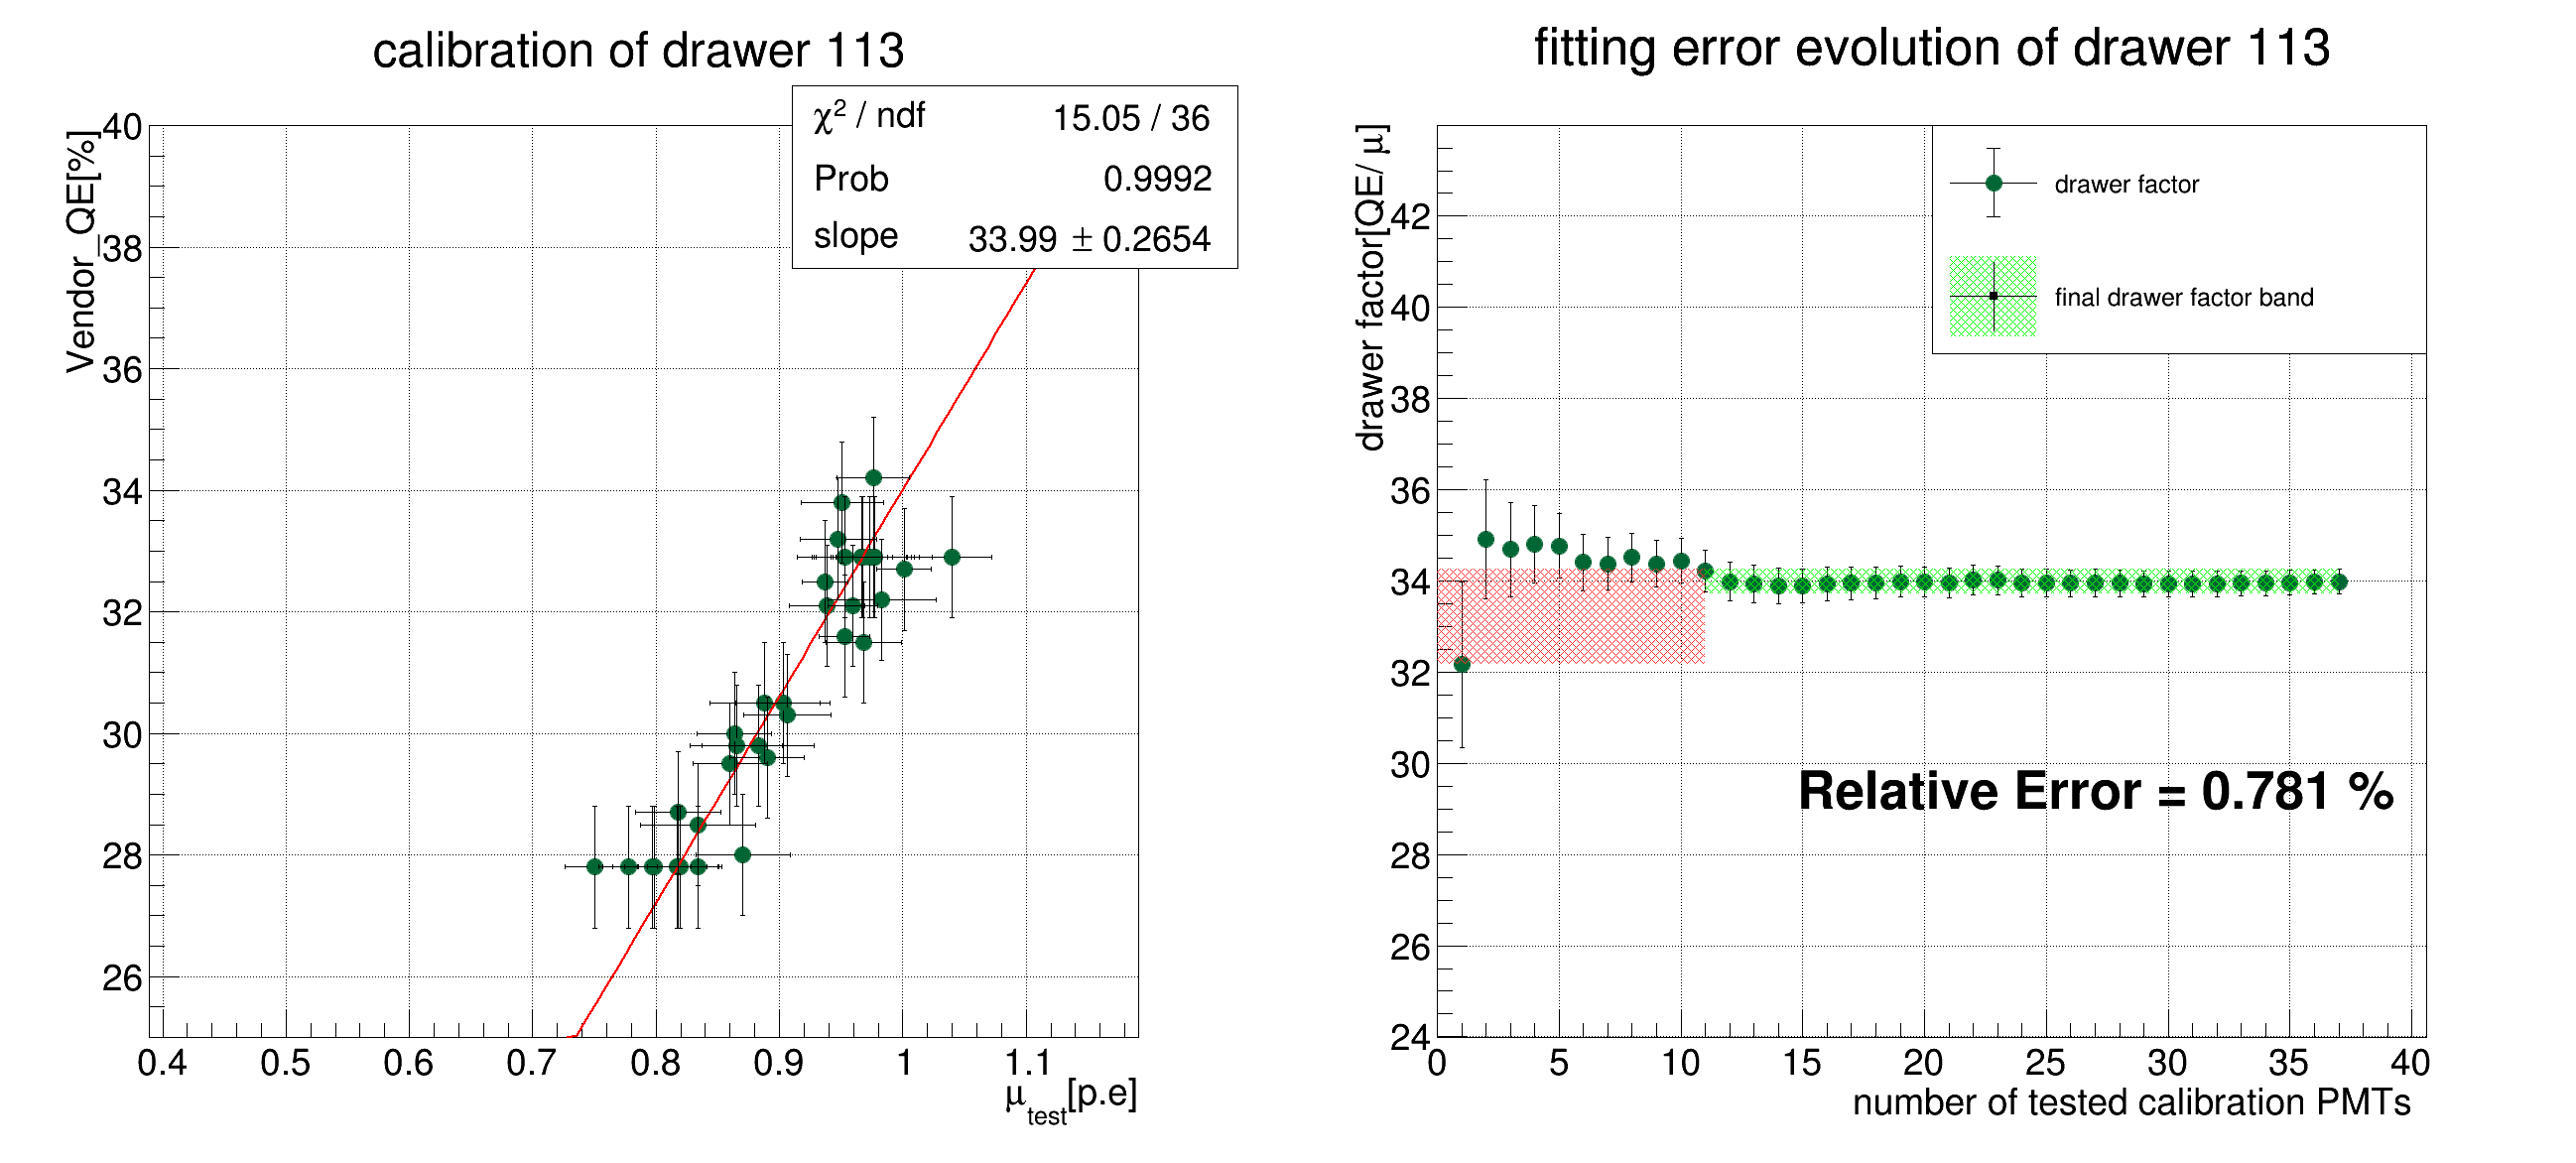
\includegraphics[width=0.45\textwidth]{sta101-12} 
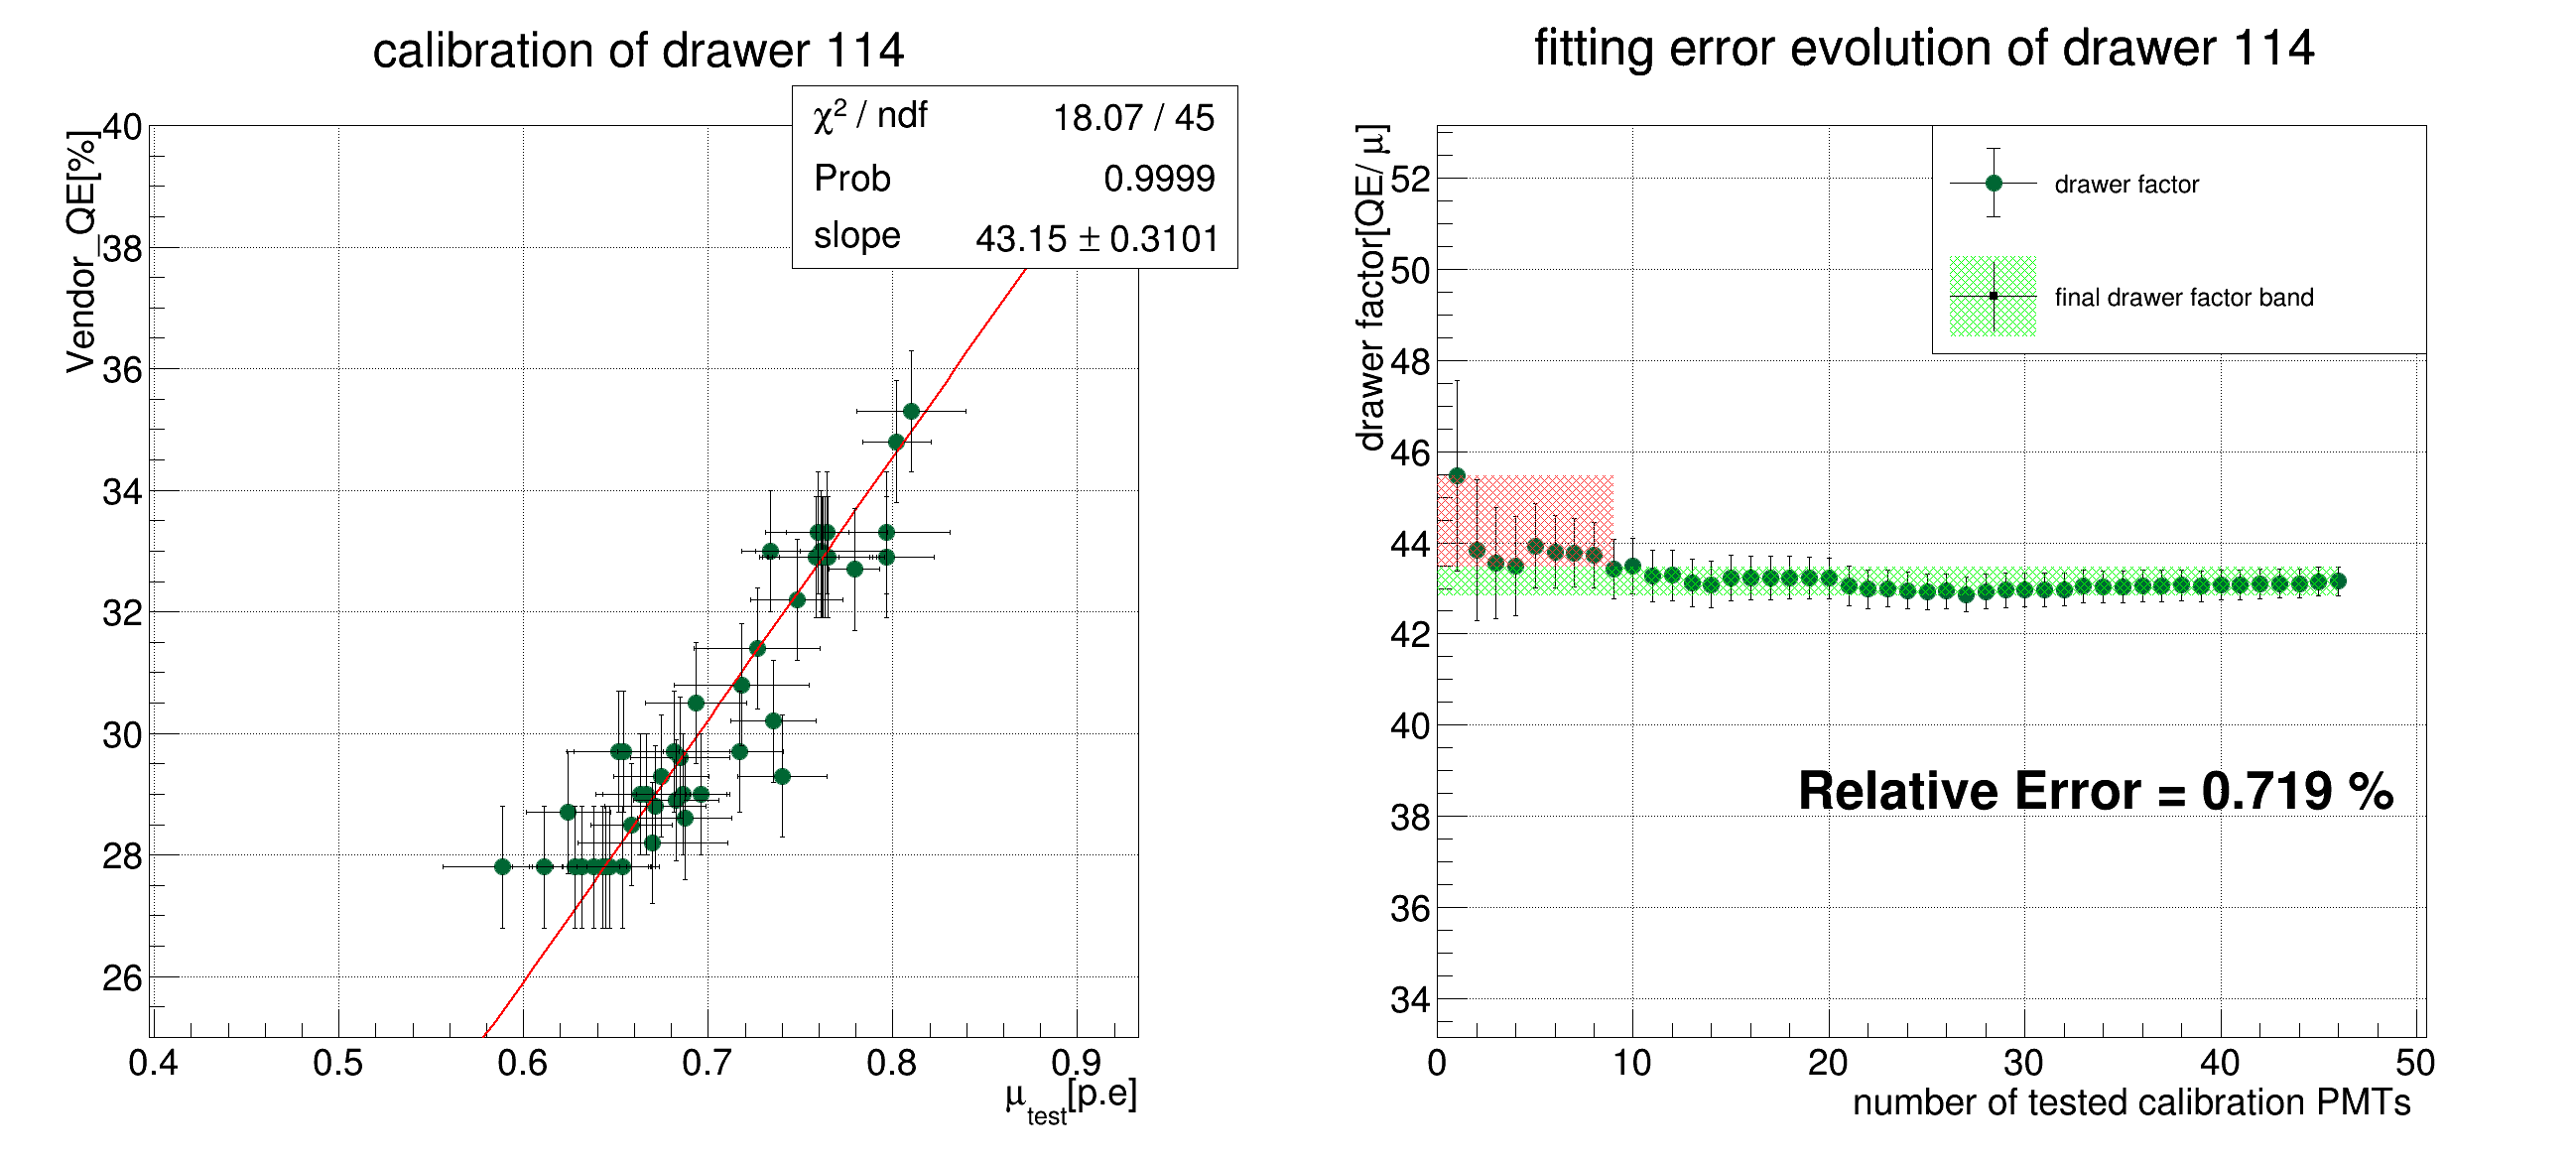
\includegraphics[width=0.45\textwidth]{sta101-13} 
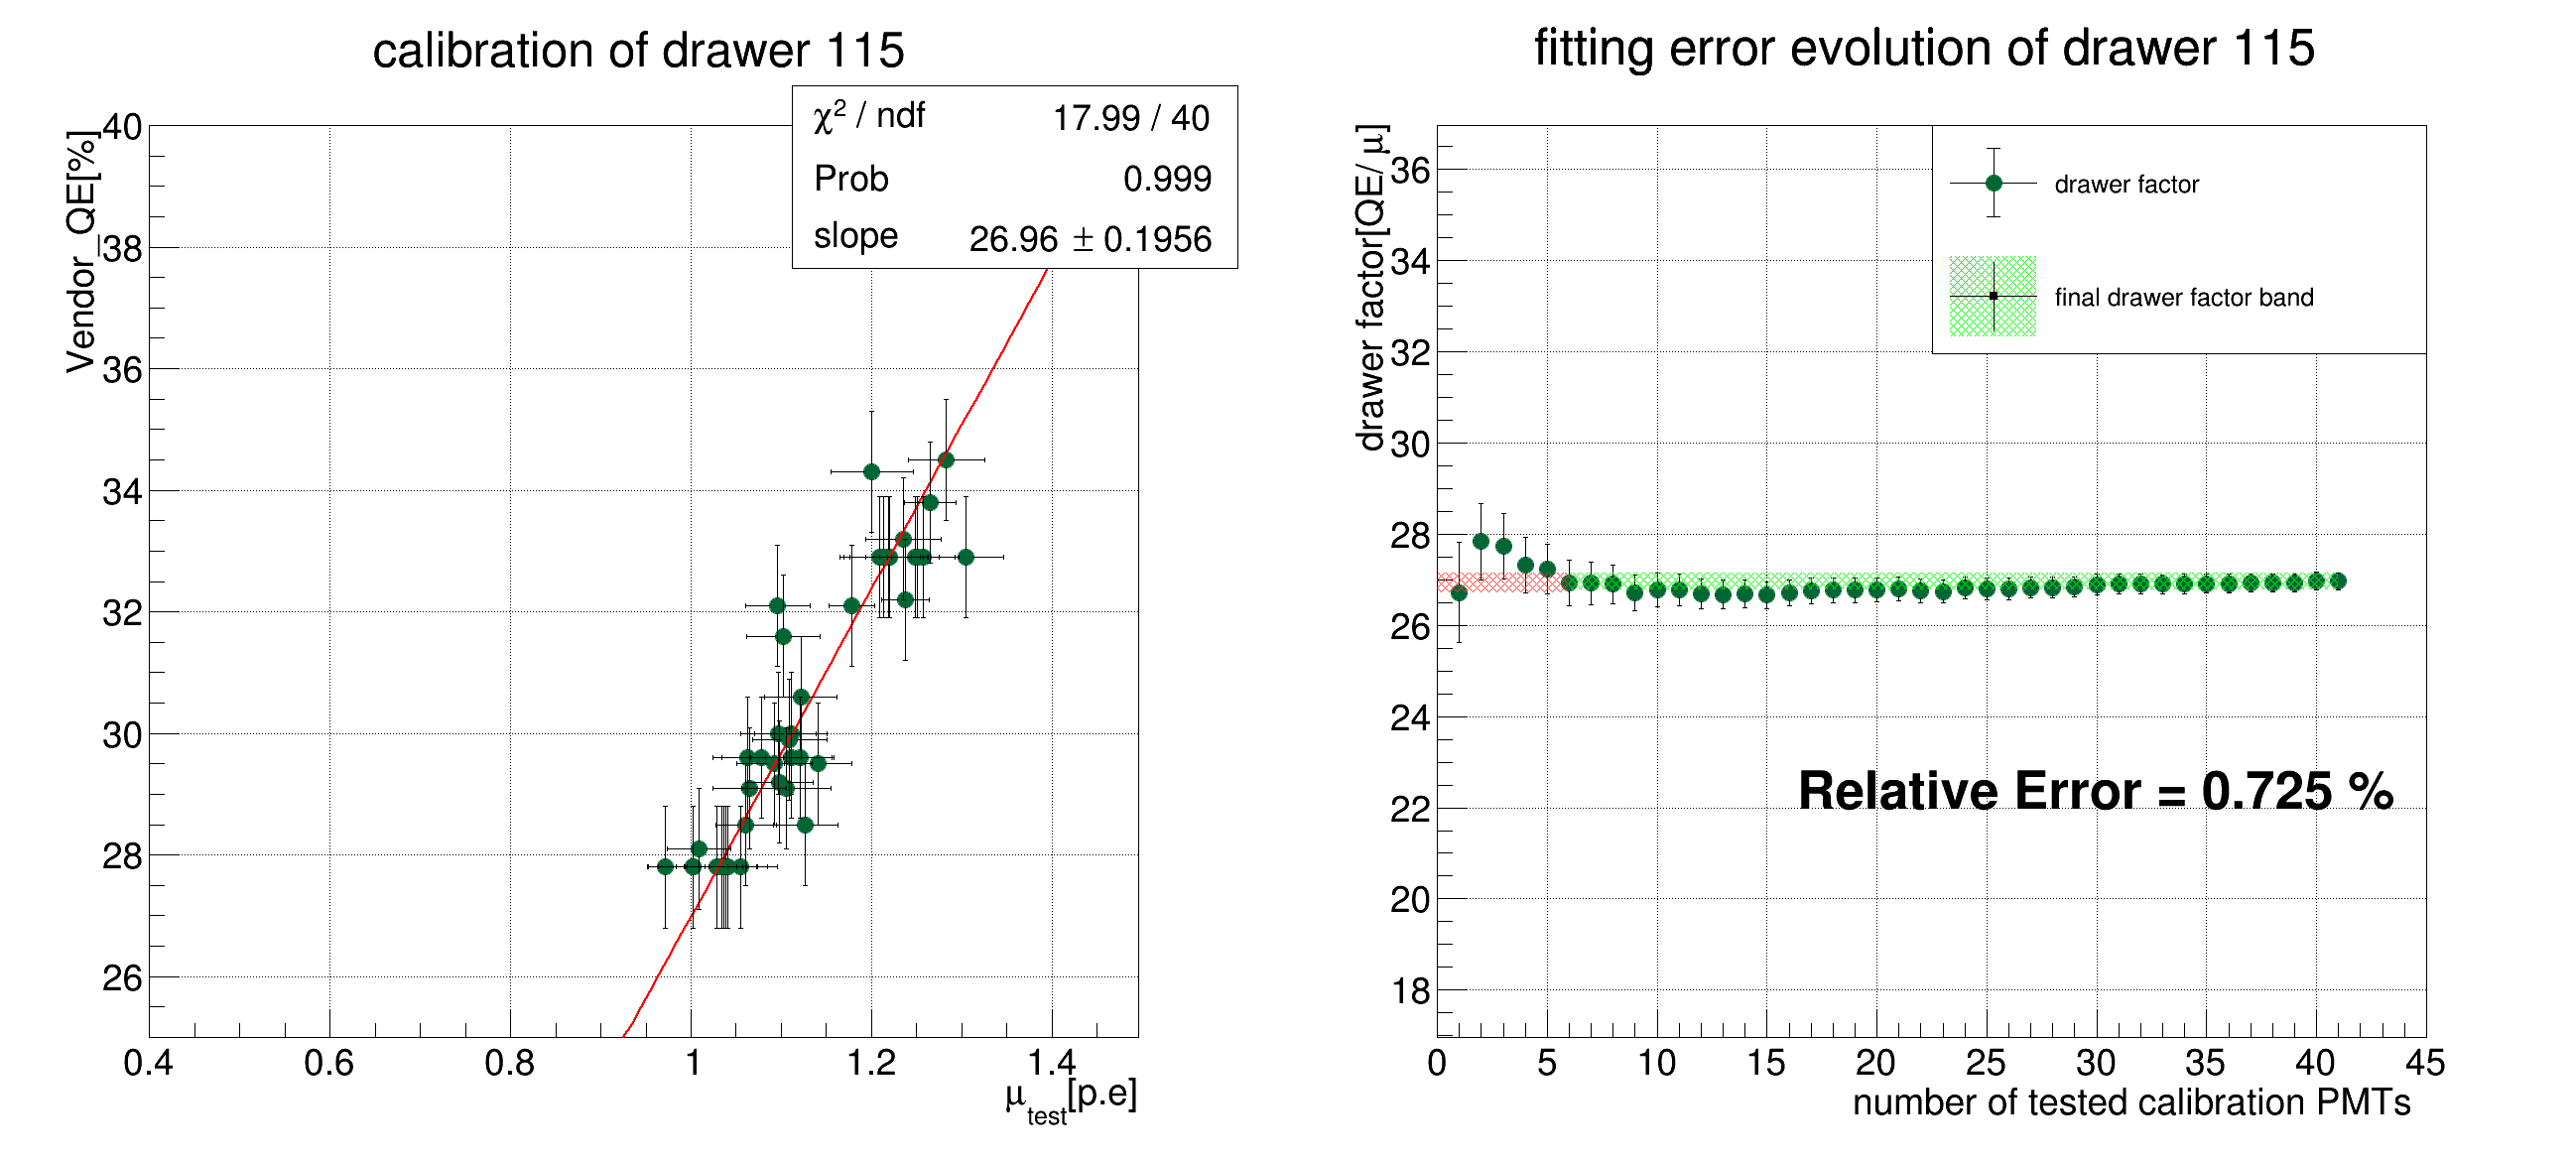
\includegraphics[width=0.45\textwidth]{sta101-14} 
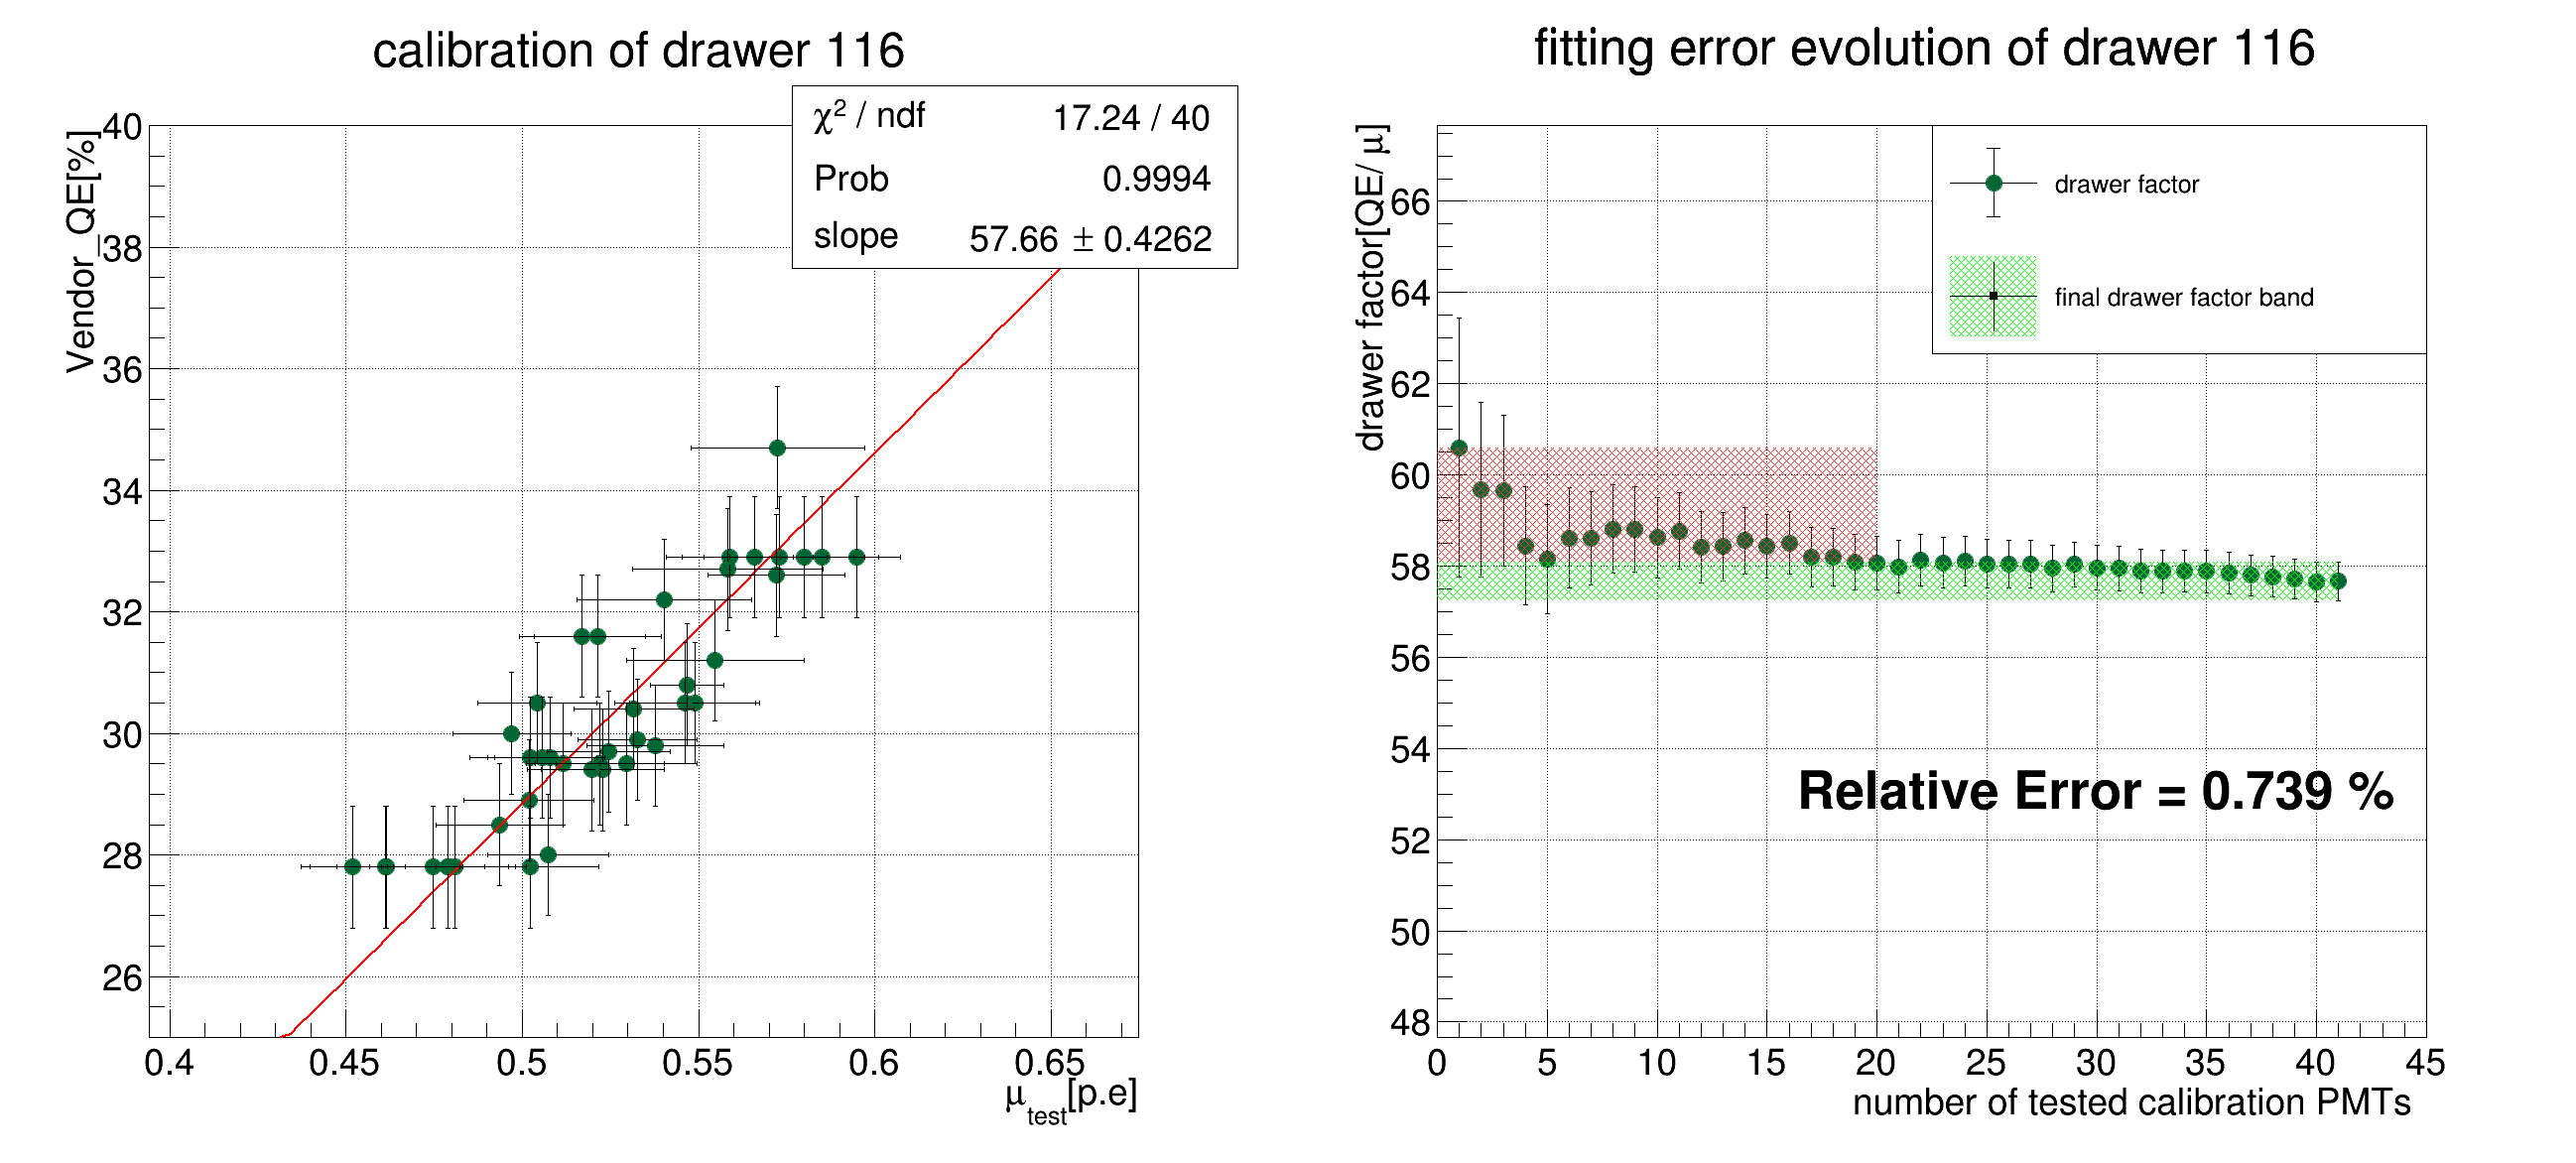
\includegraphics[width=0.45\textwidth]{sta101-15} 
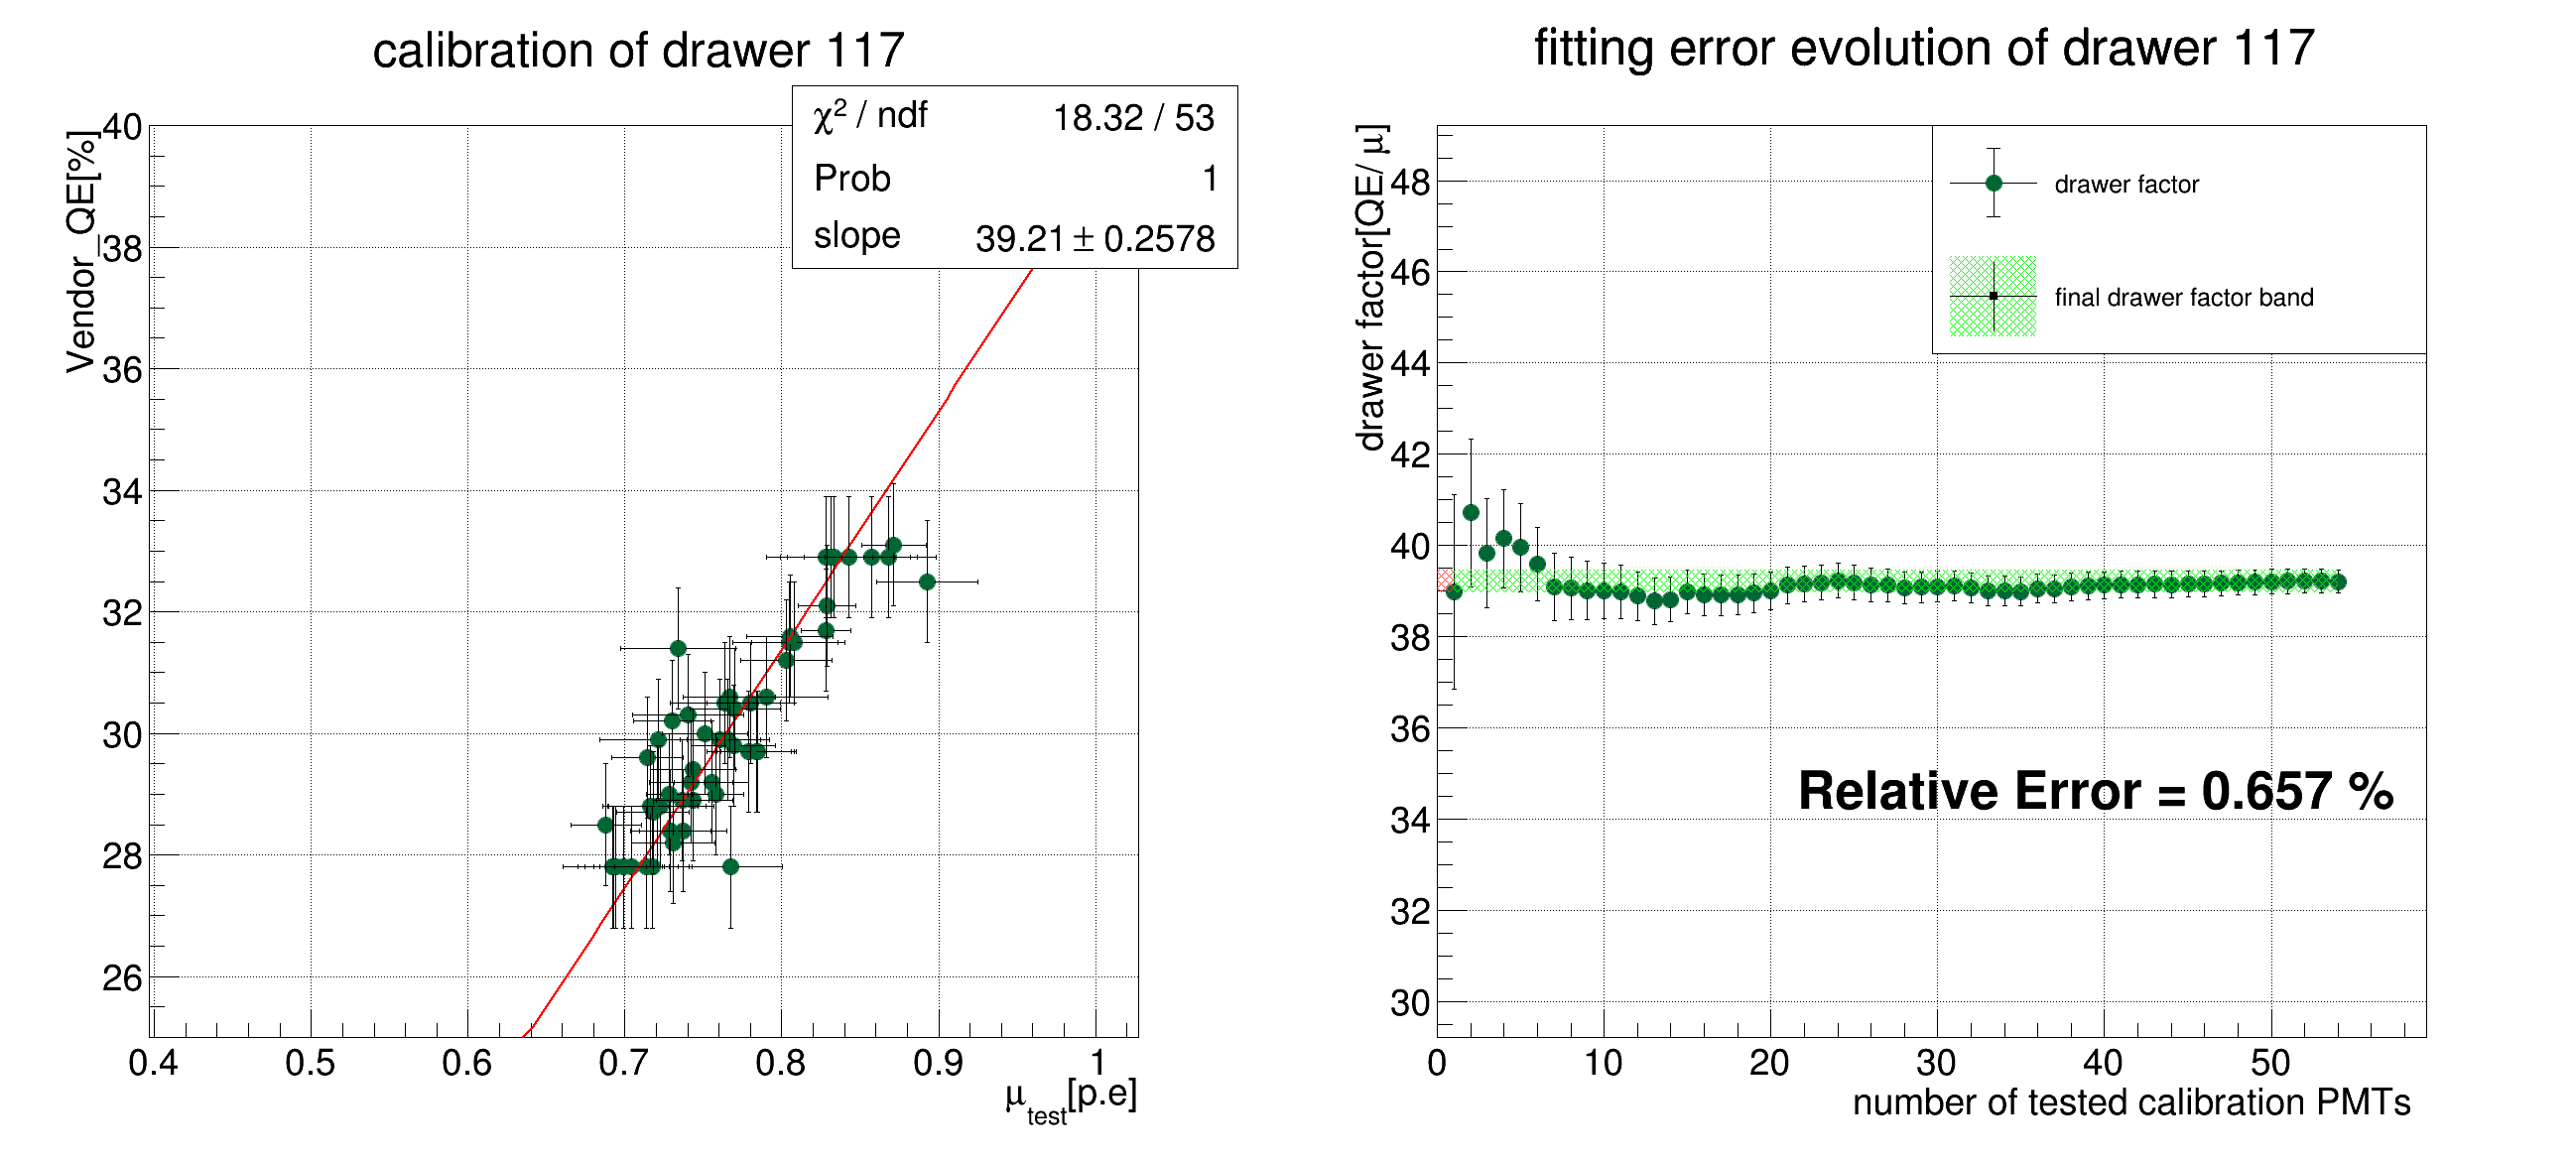
\includegraphics[width=0.45\textwidth]{sta101-16} 
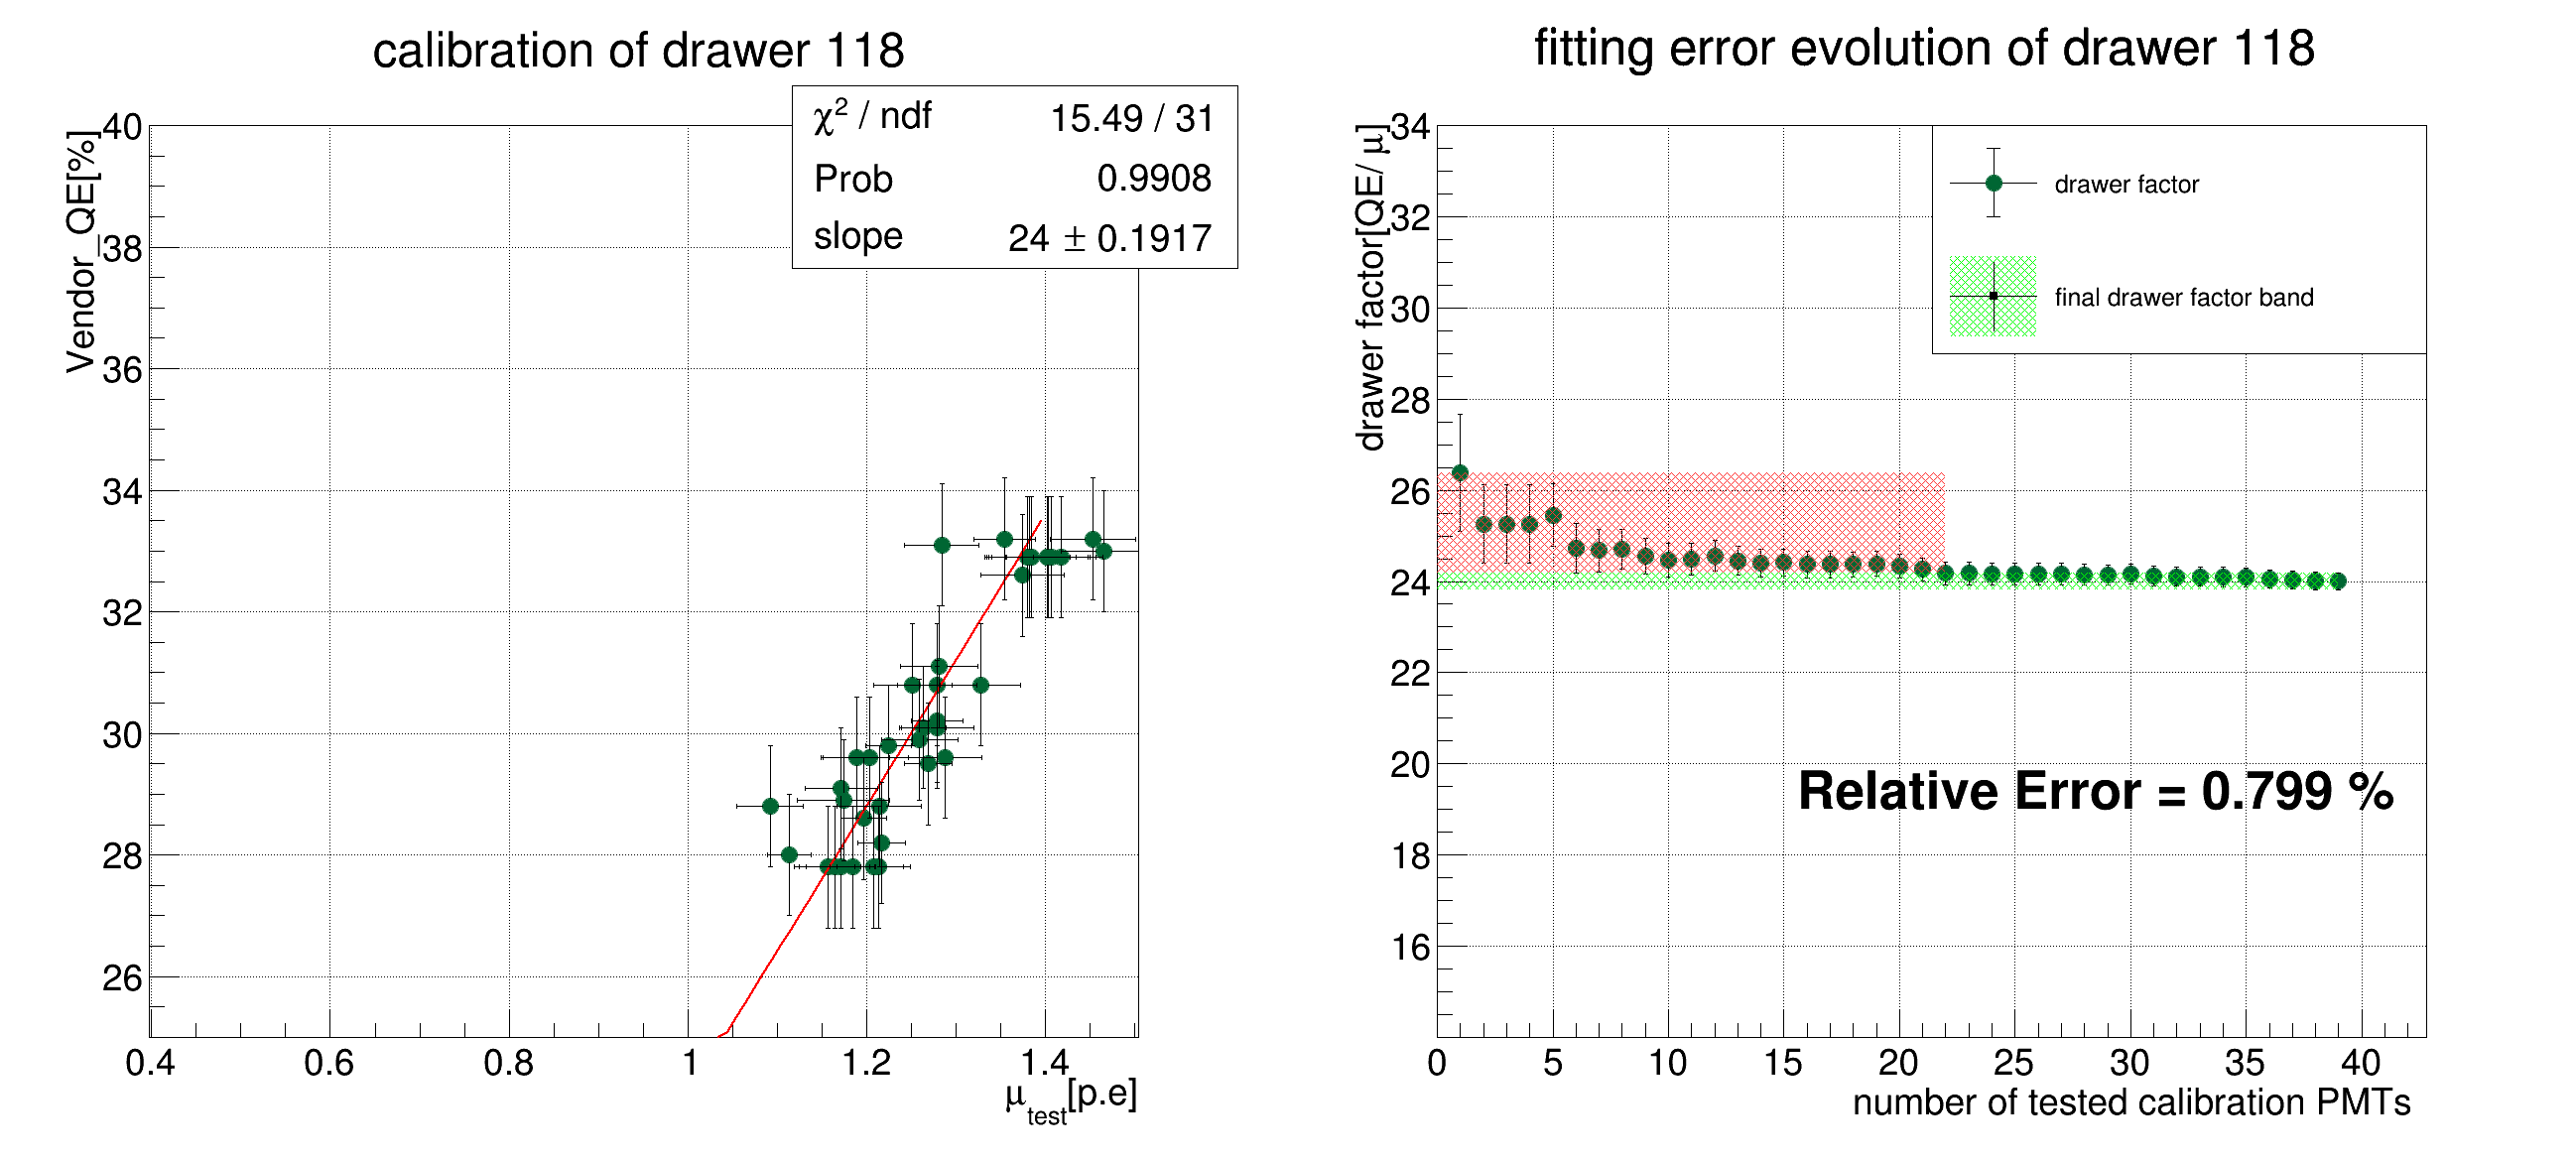
\includegraphics[width=0.45\textwidth]{sta101-17} 
\end{frame}
\begin{frame}{drawer-calibration}
\vspace{-.5cm}
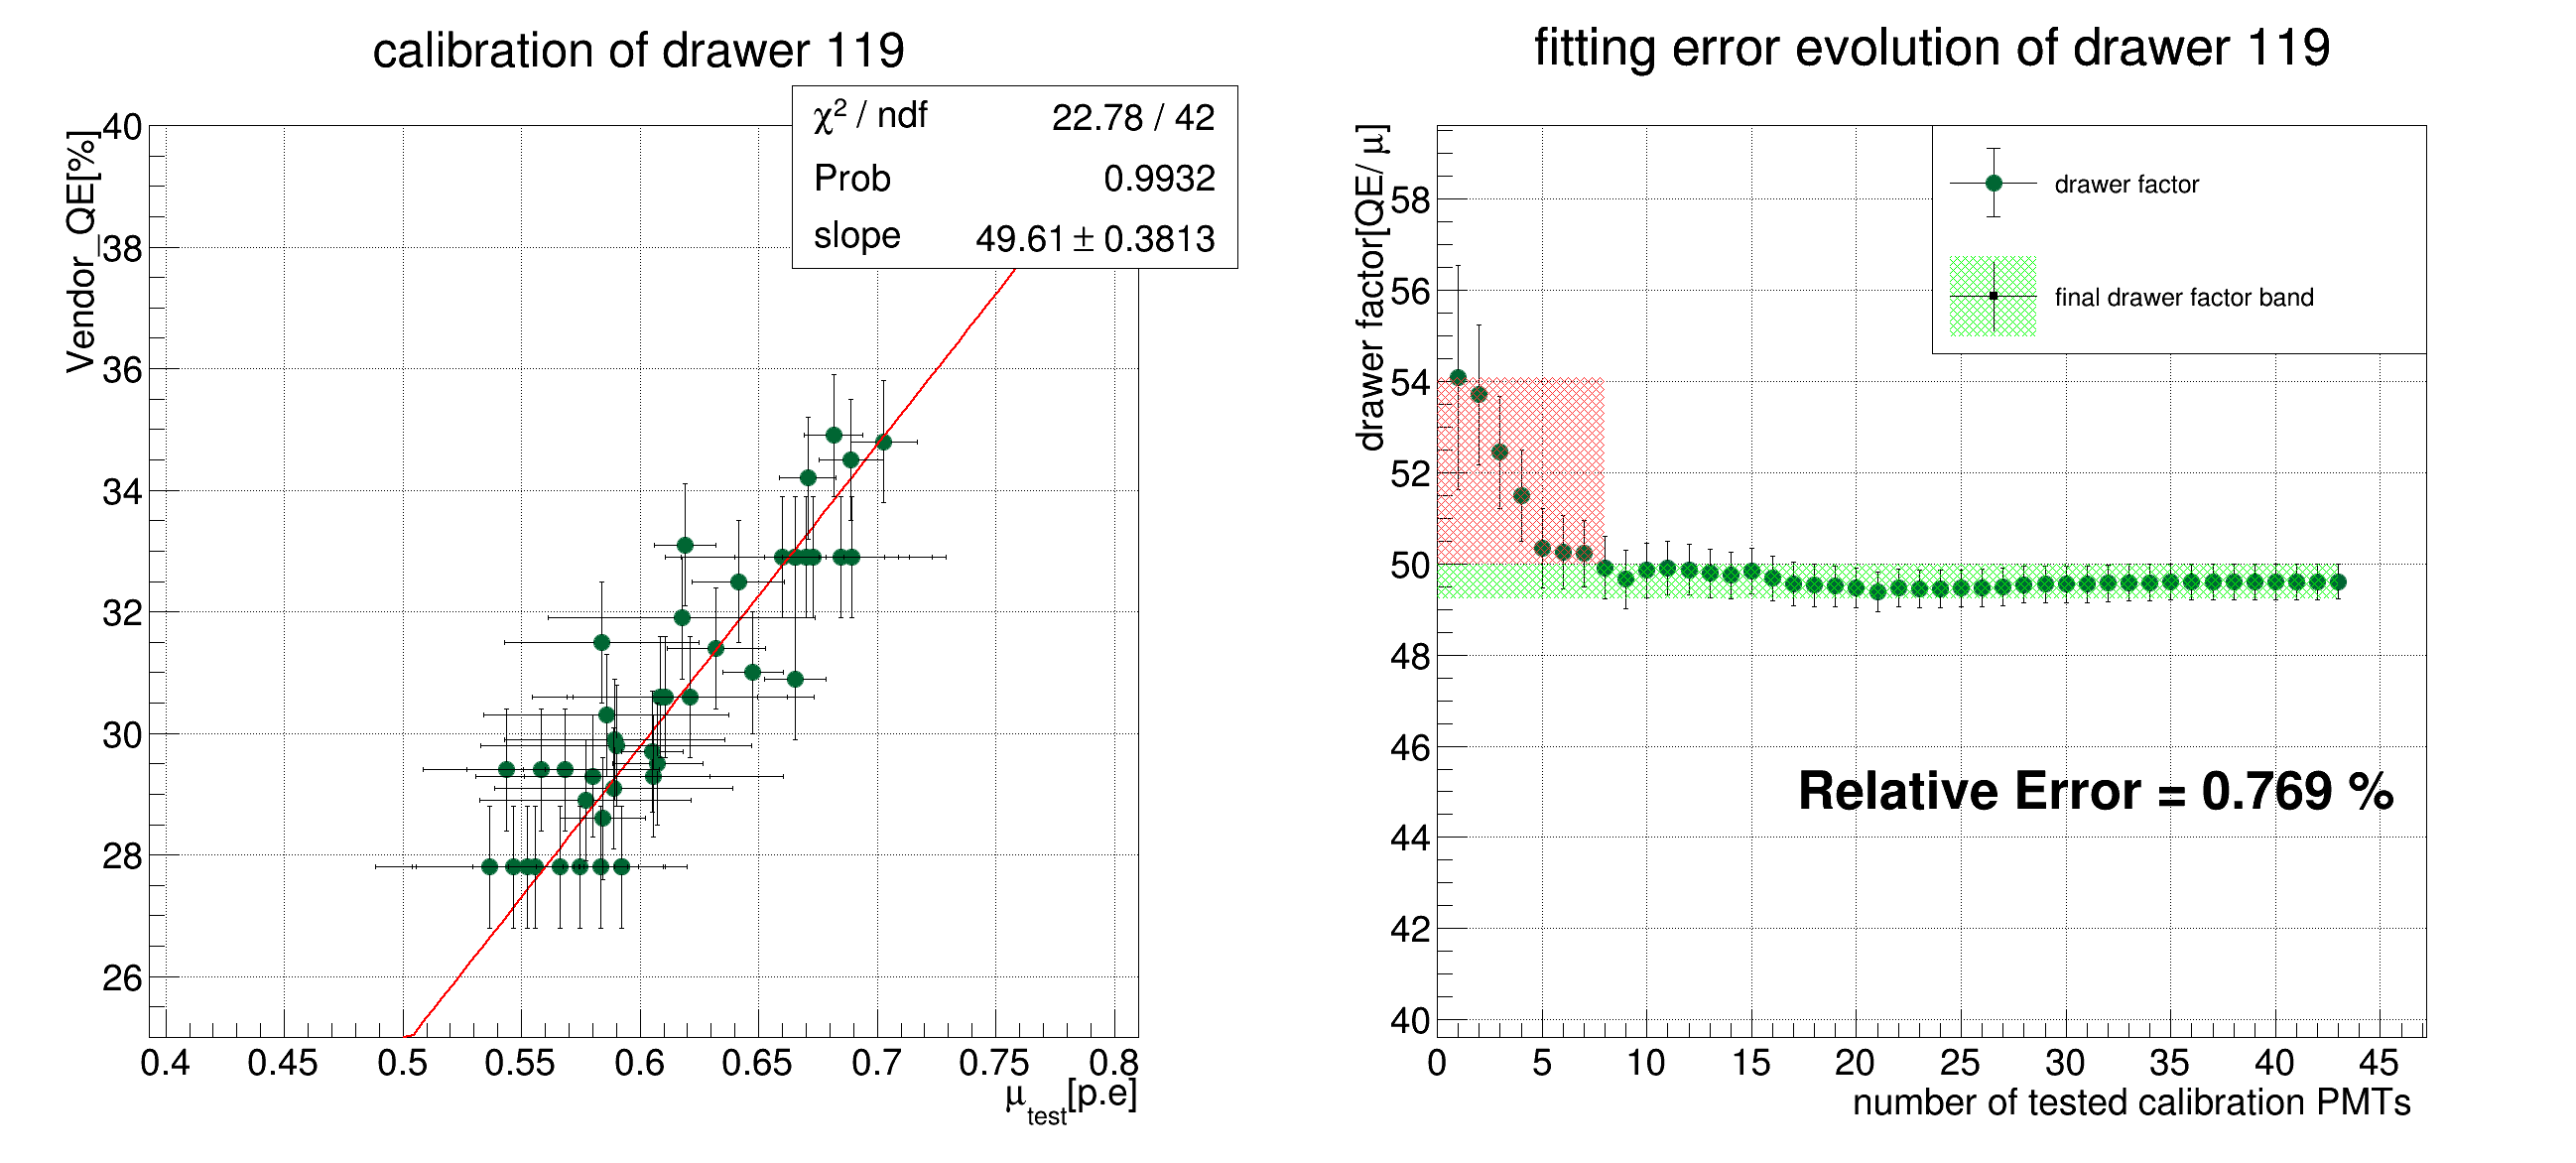
\includegraphics[width=0.45\textwidth]{sta101-18} 
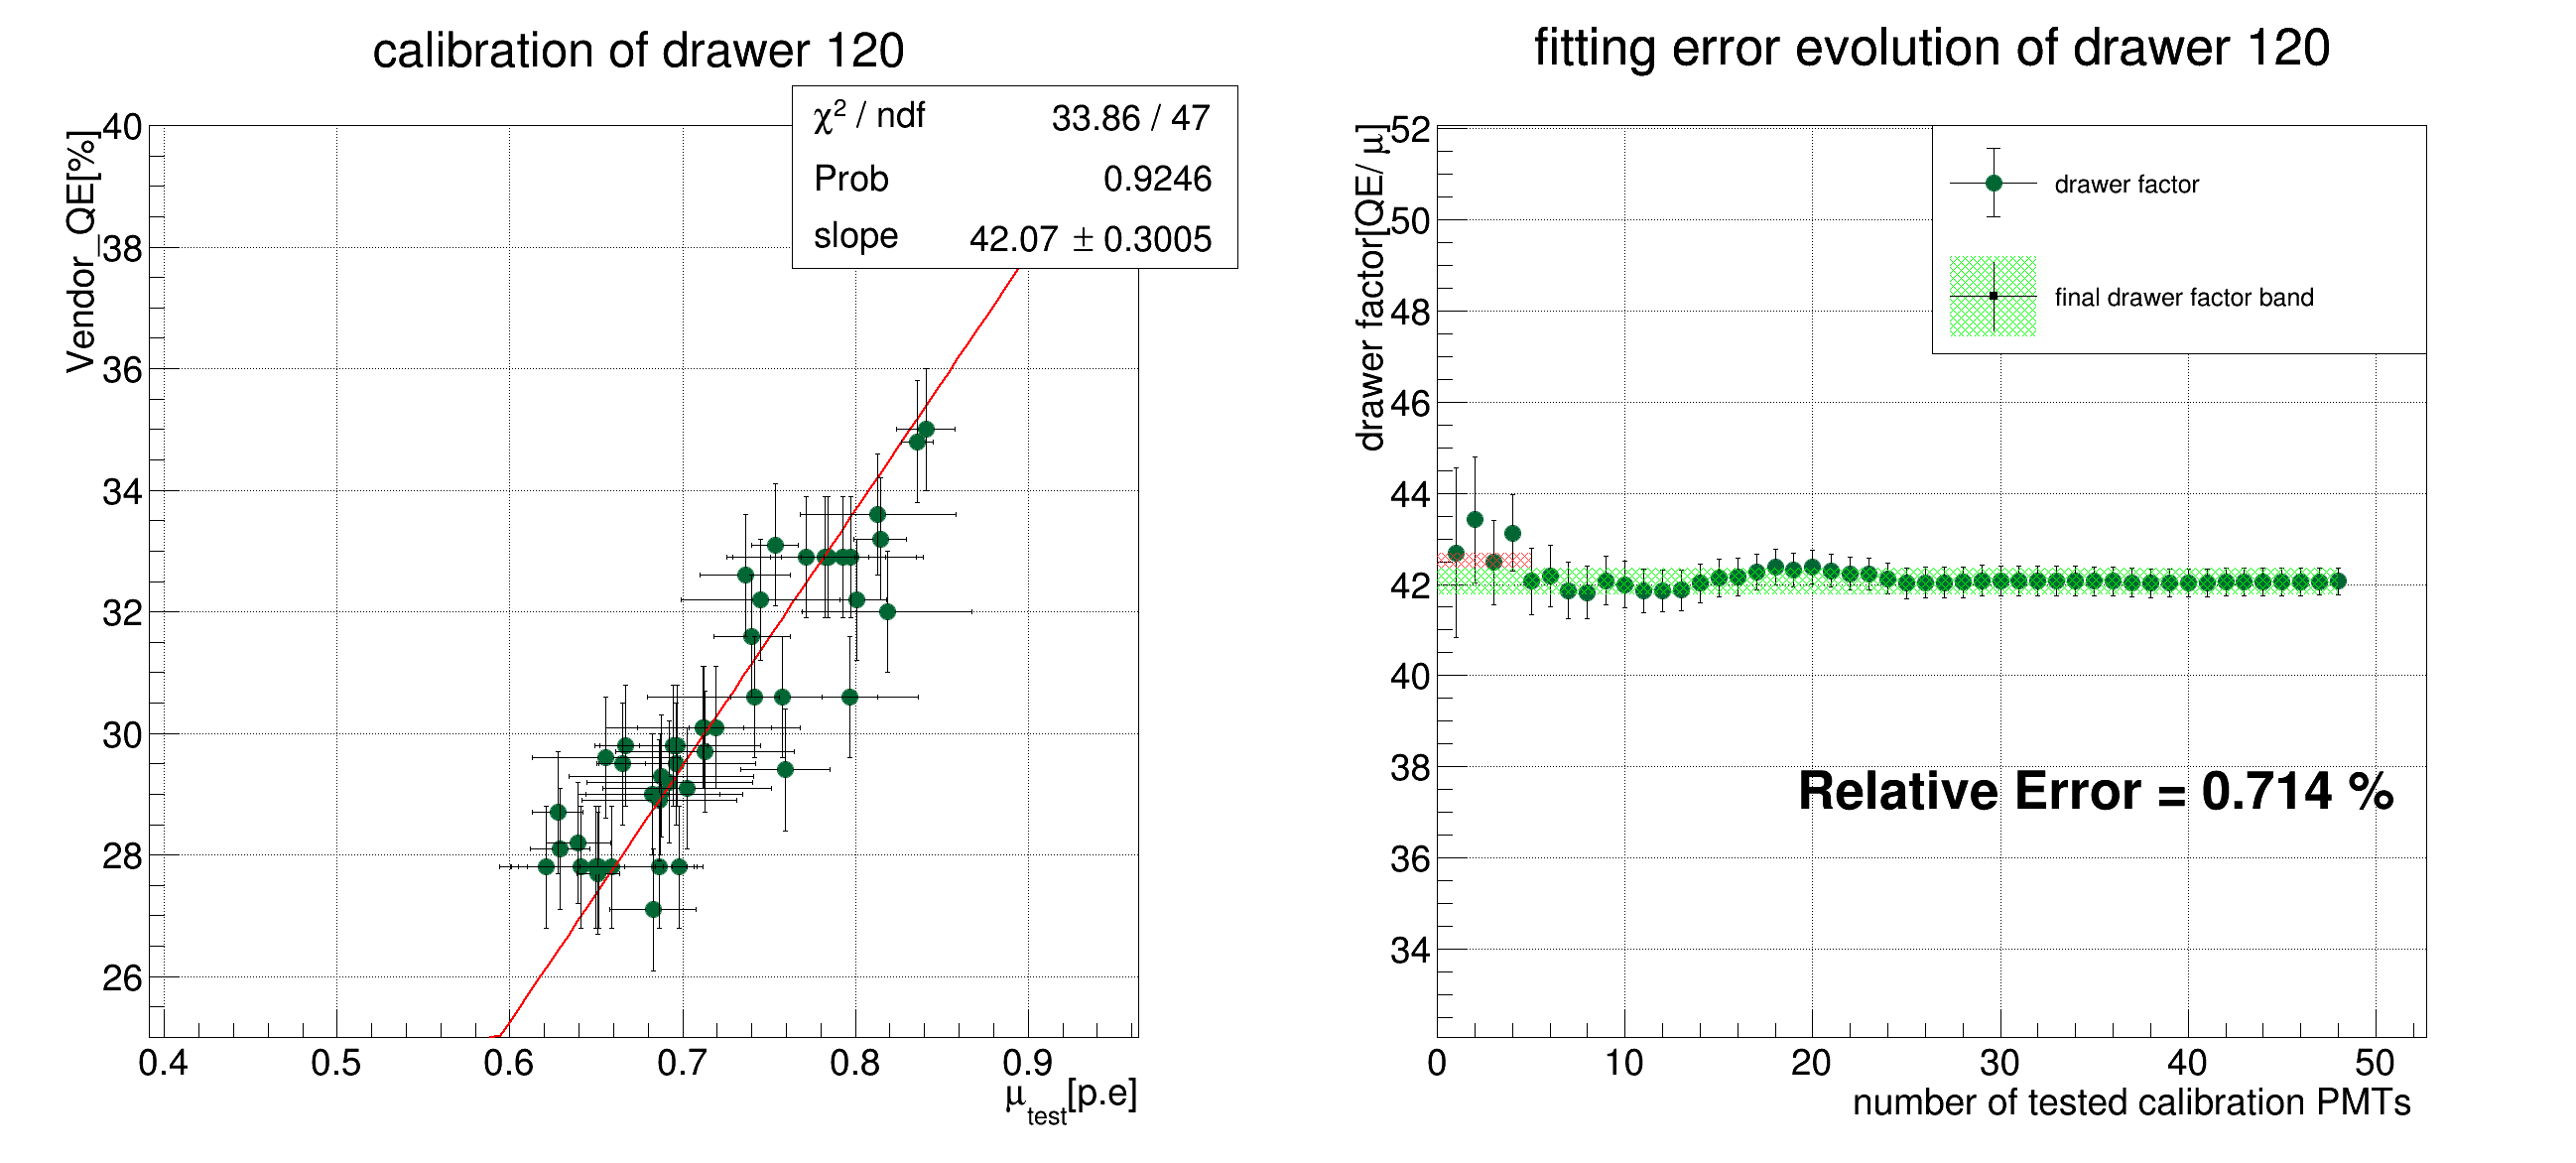
\includegraphics[width=0.45\textwidth]{sta101-19} 
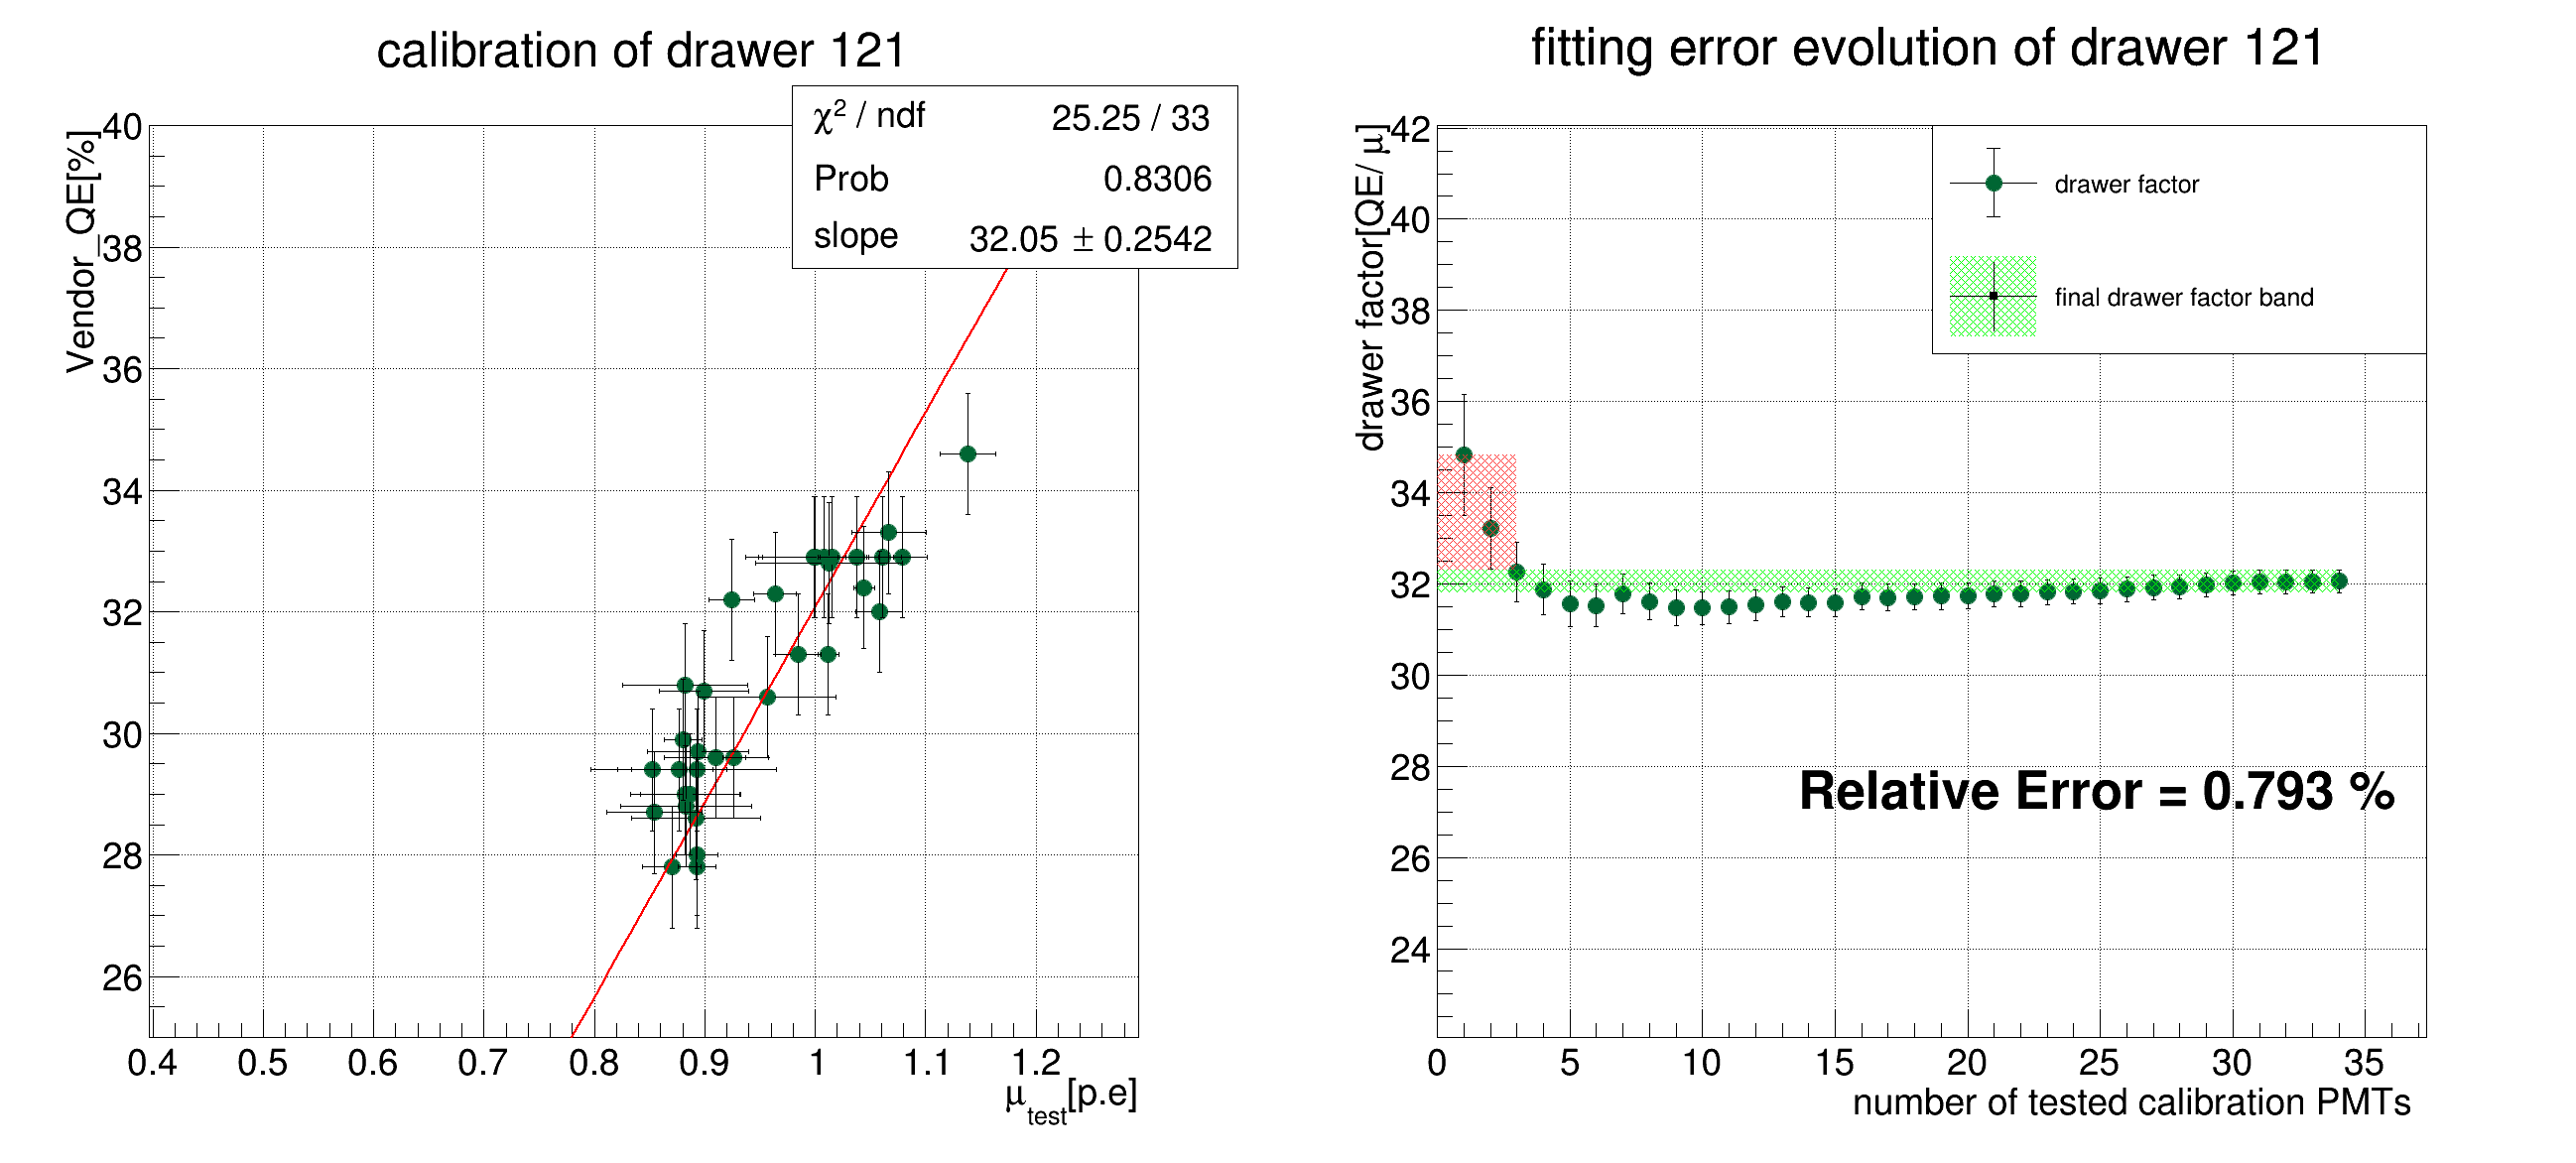
\includegraphics[width=0.45\textwidth]{sta101-20} 
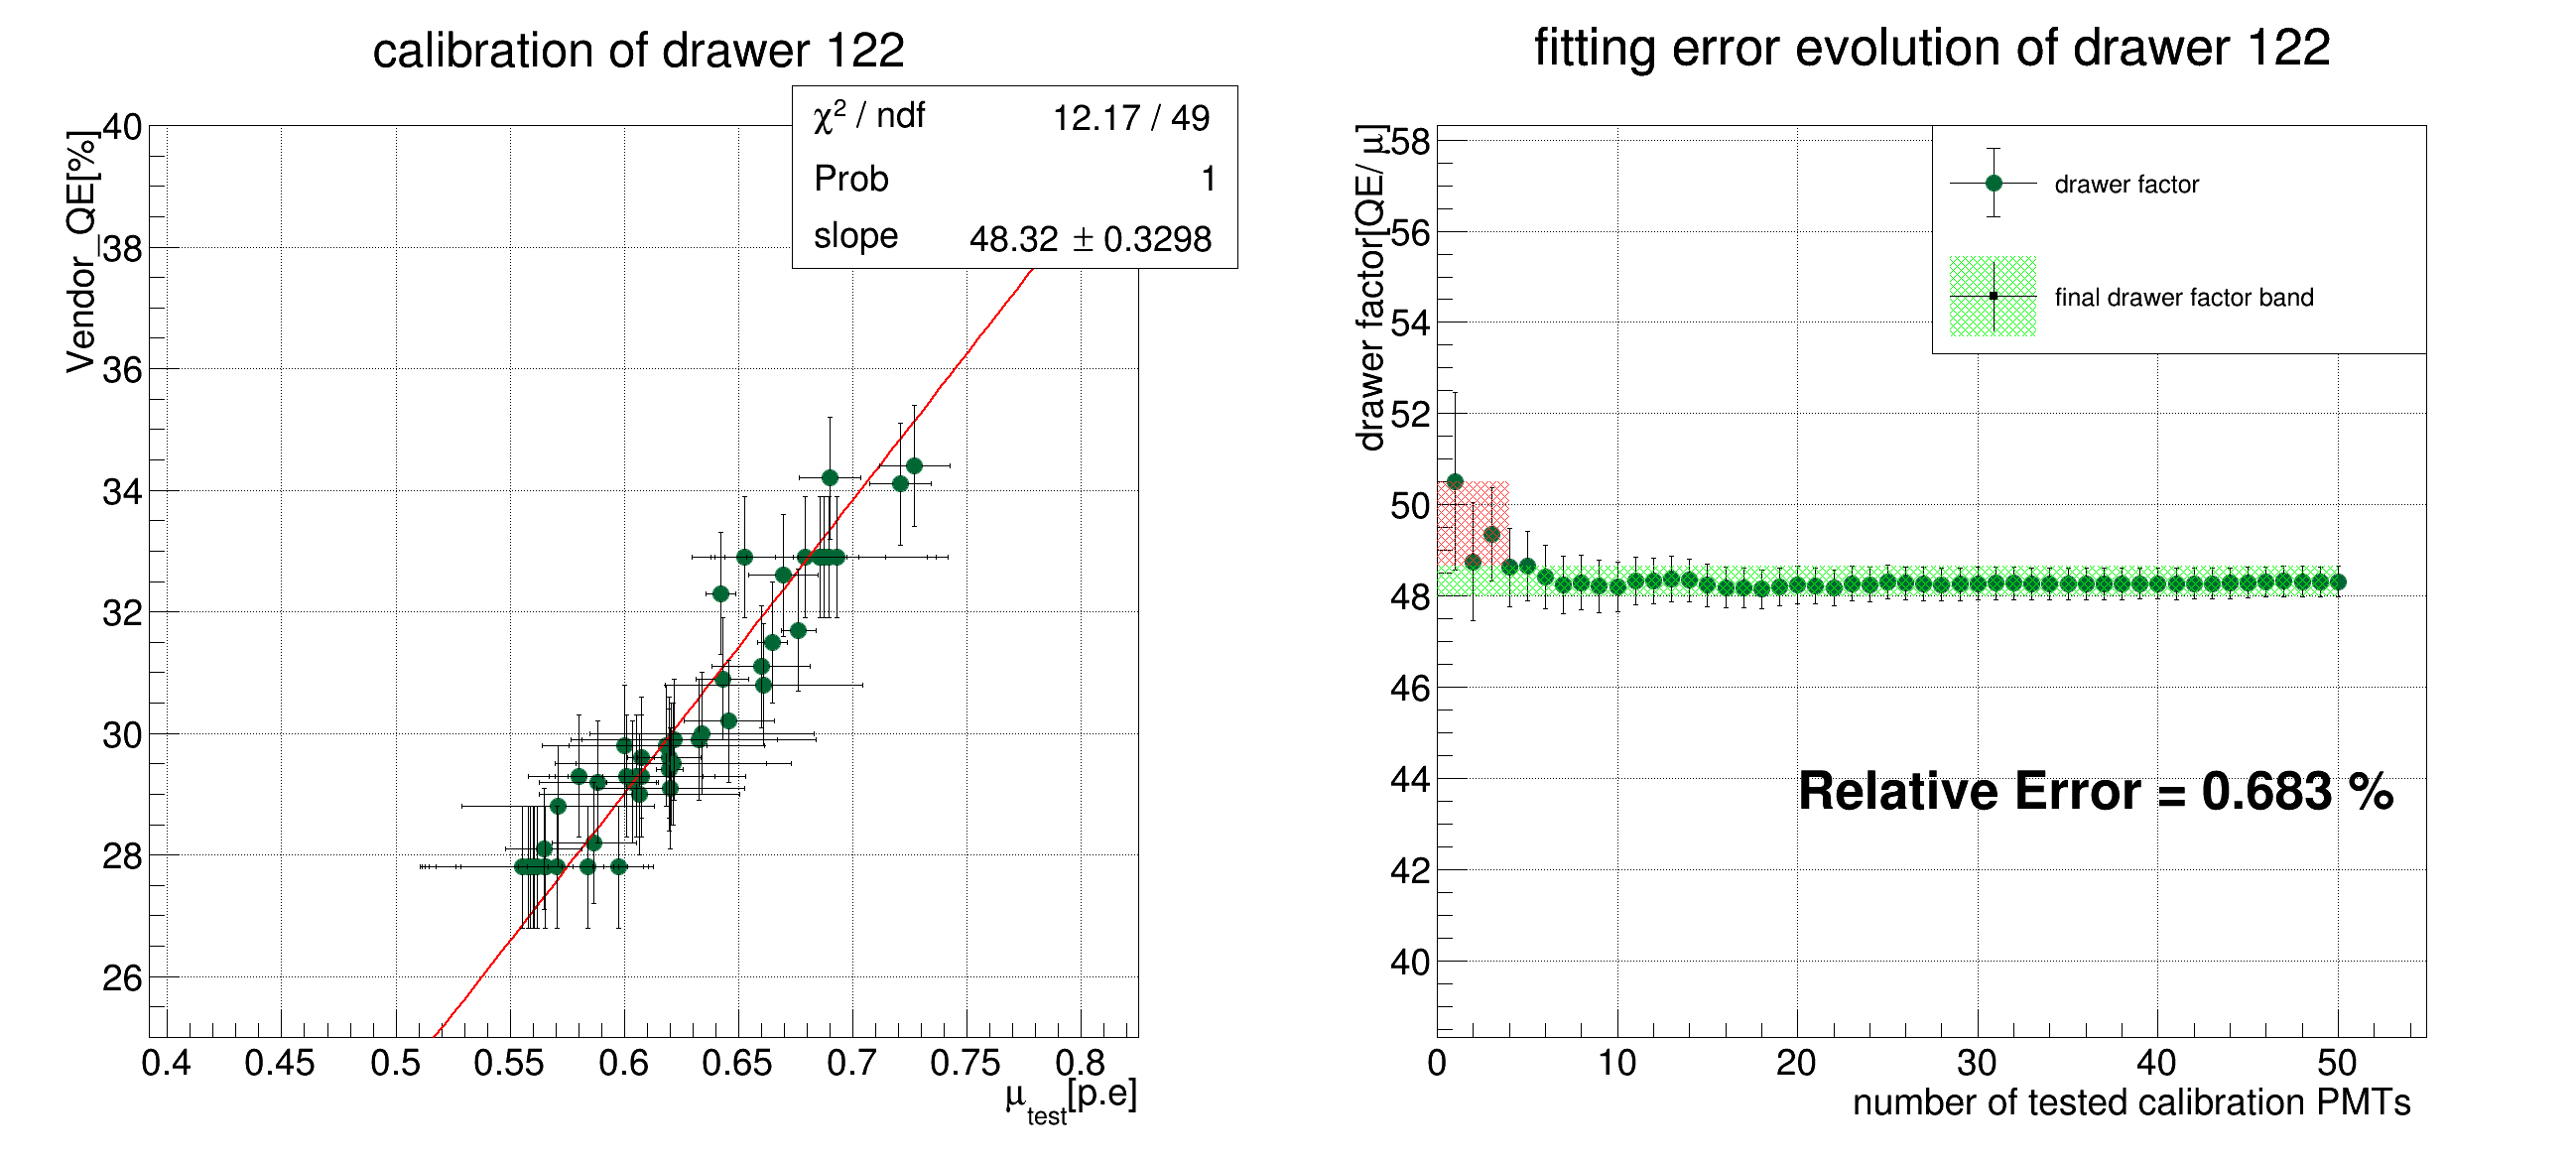
\includegraphics[width=0.45\textwidth]{sta101-21} 
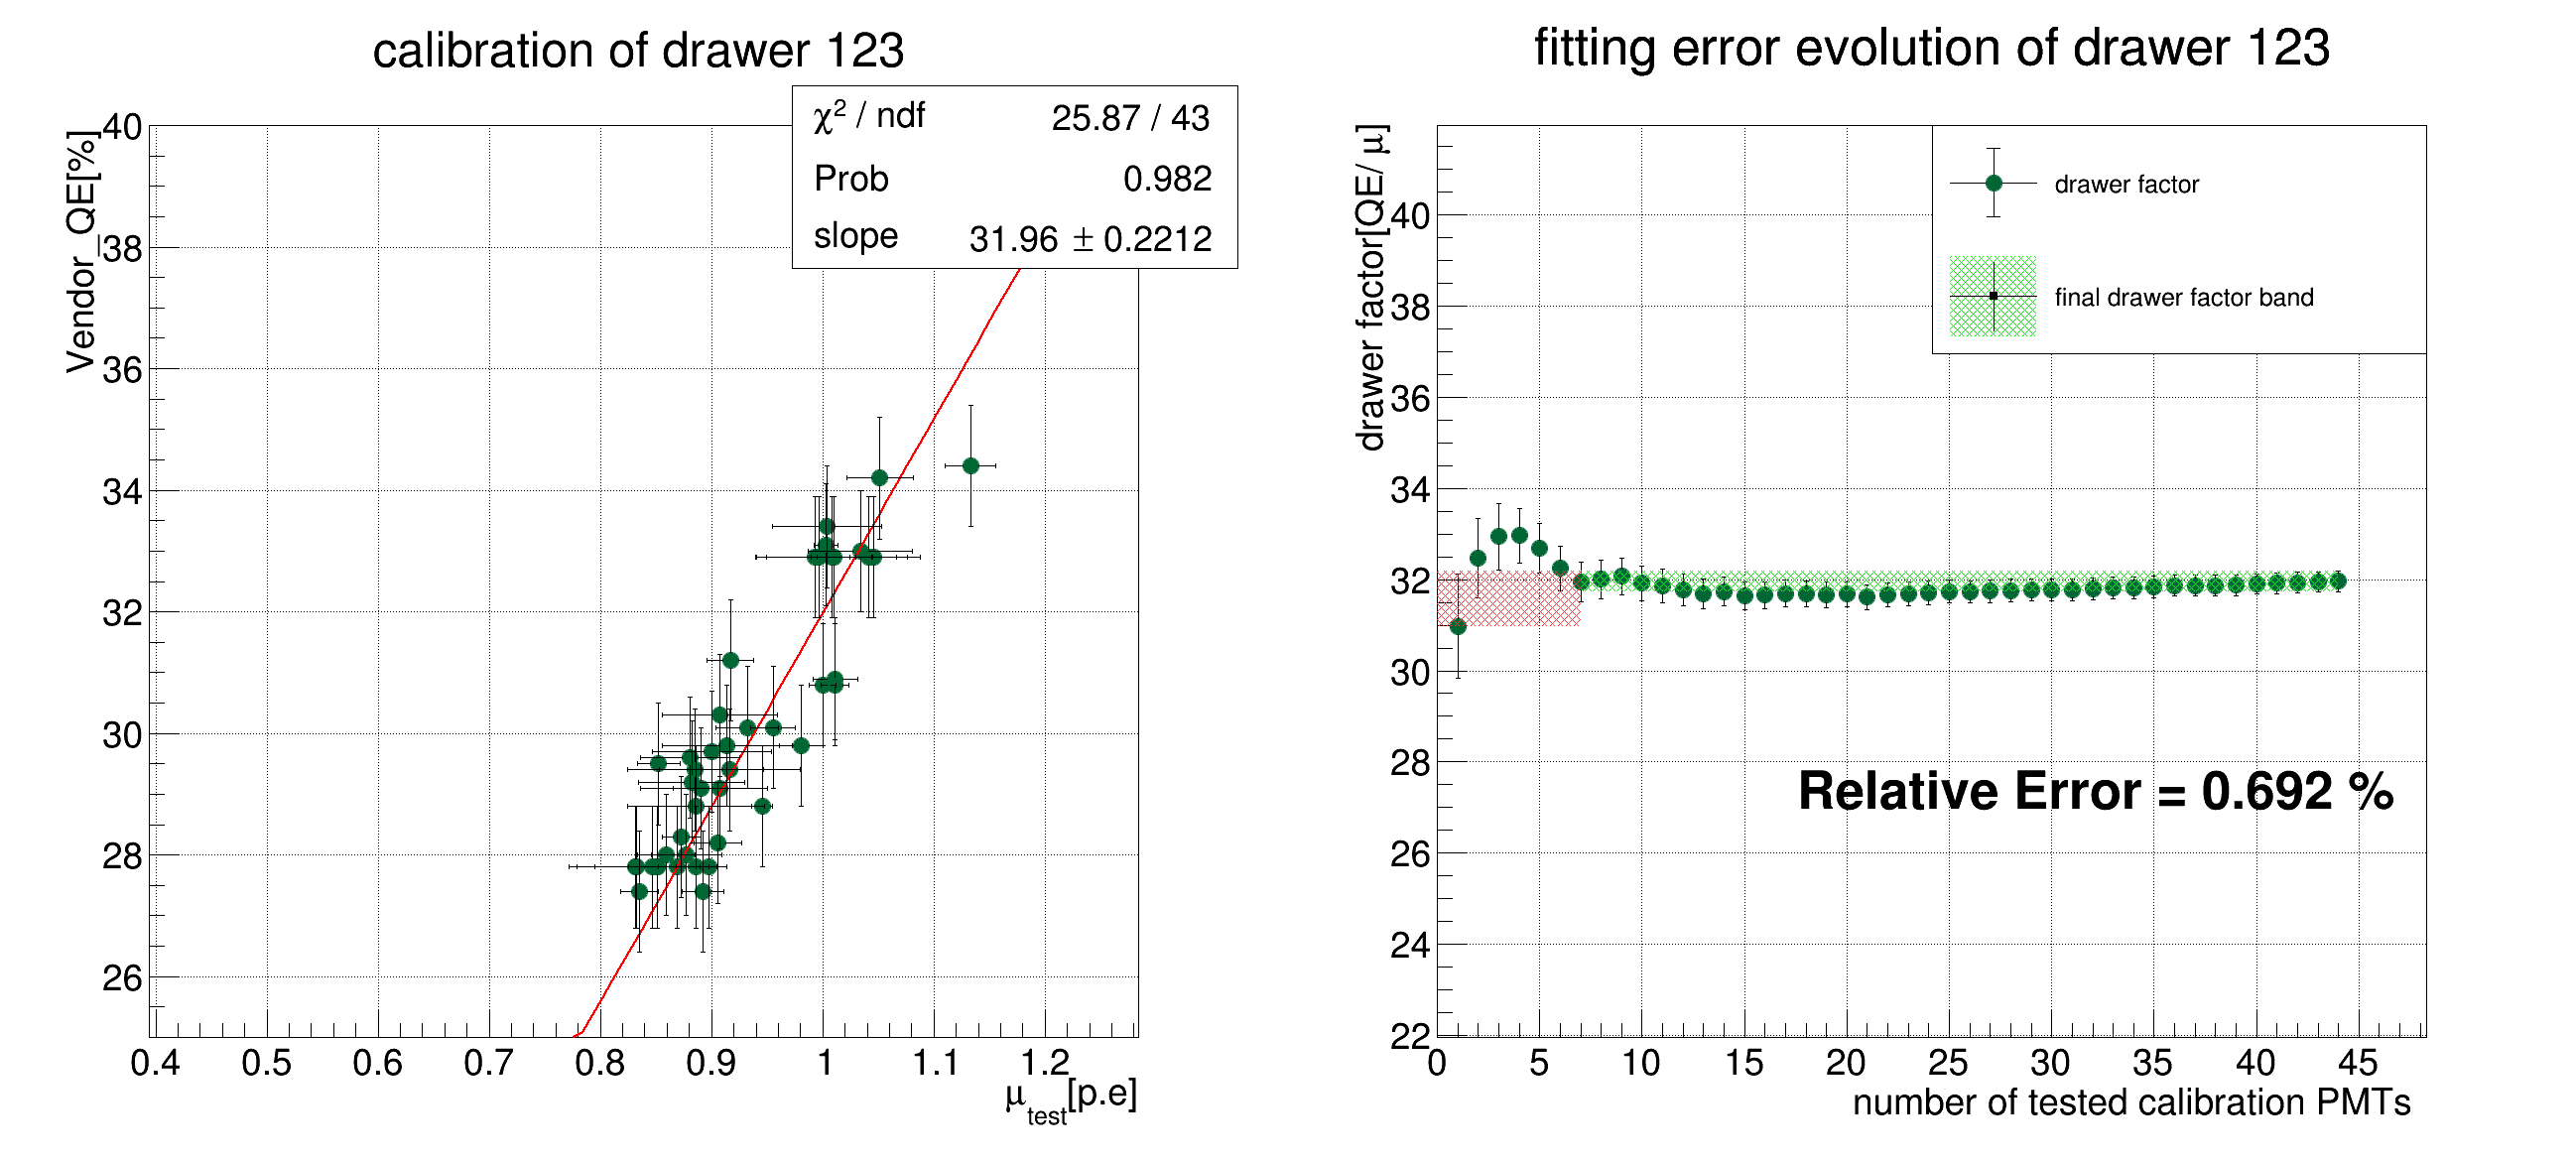
\includegraphics[width=0.45\textwidth]{sta101-22} 
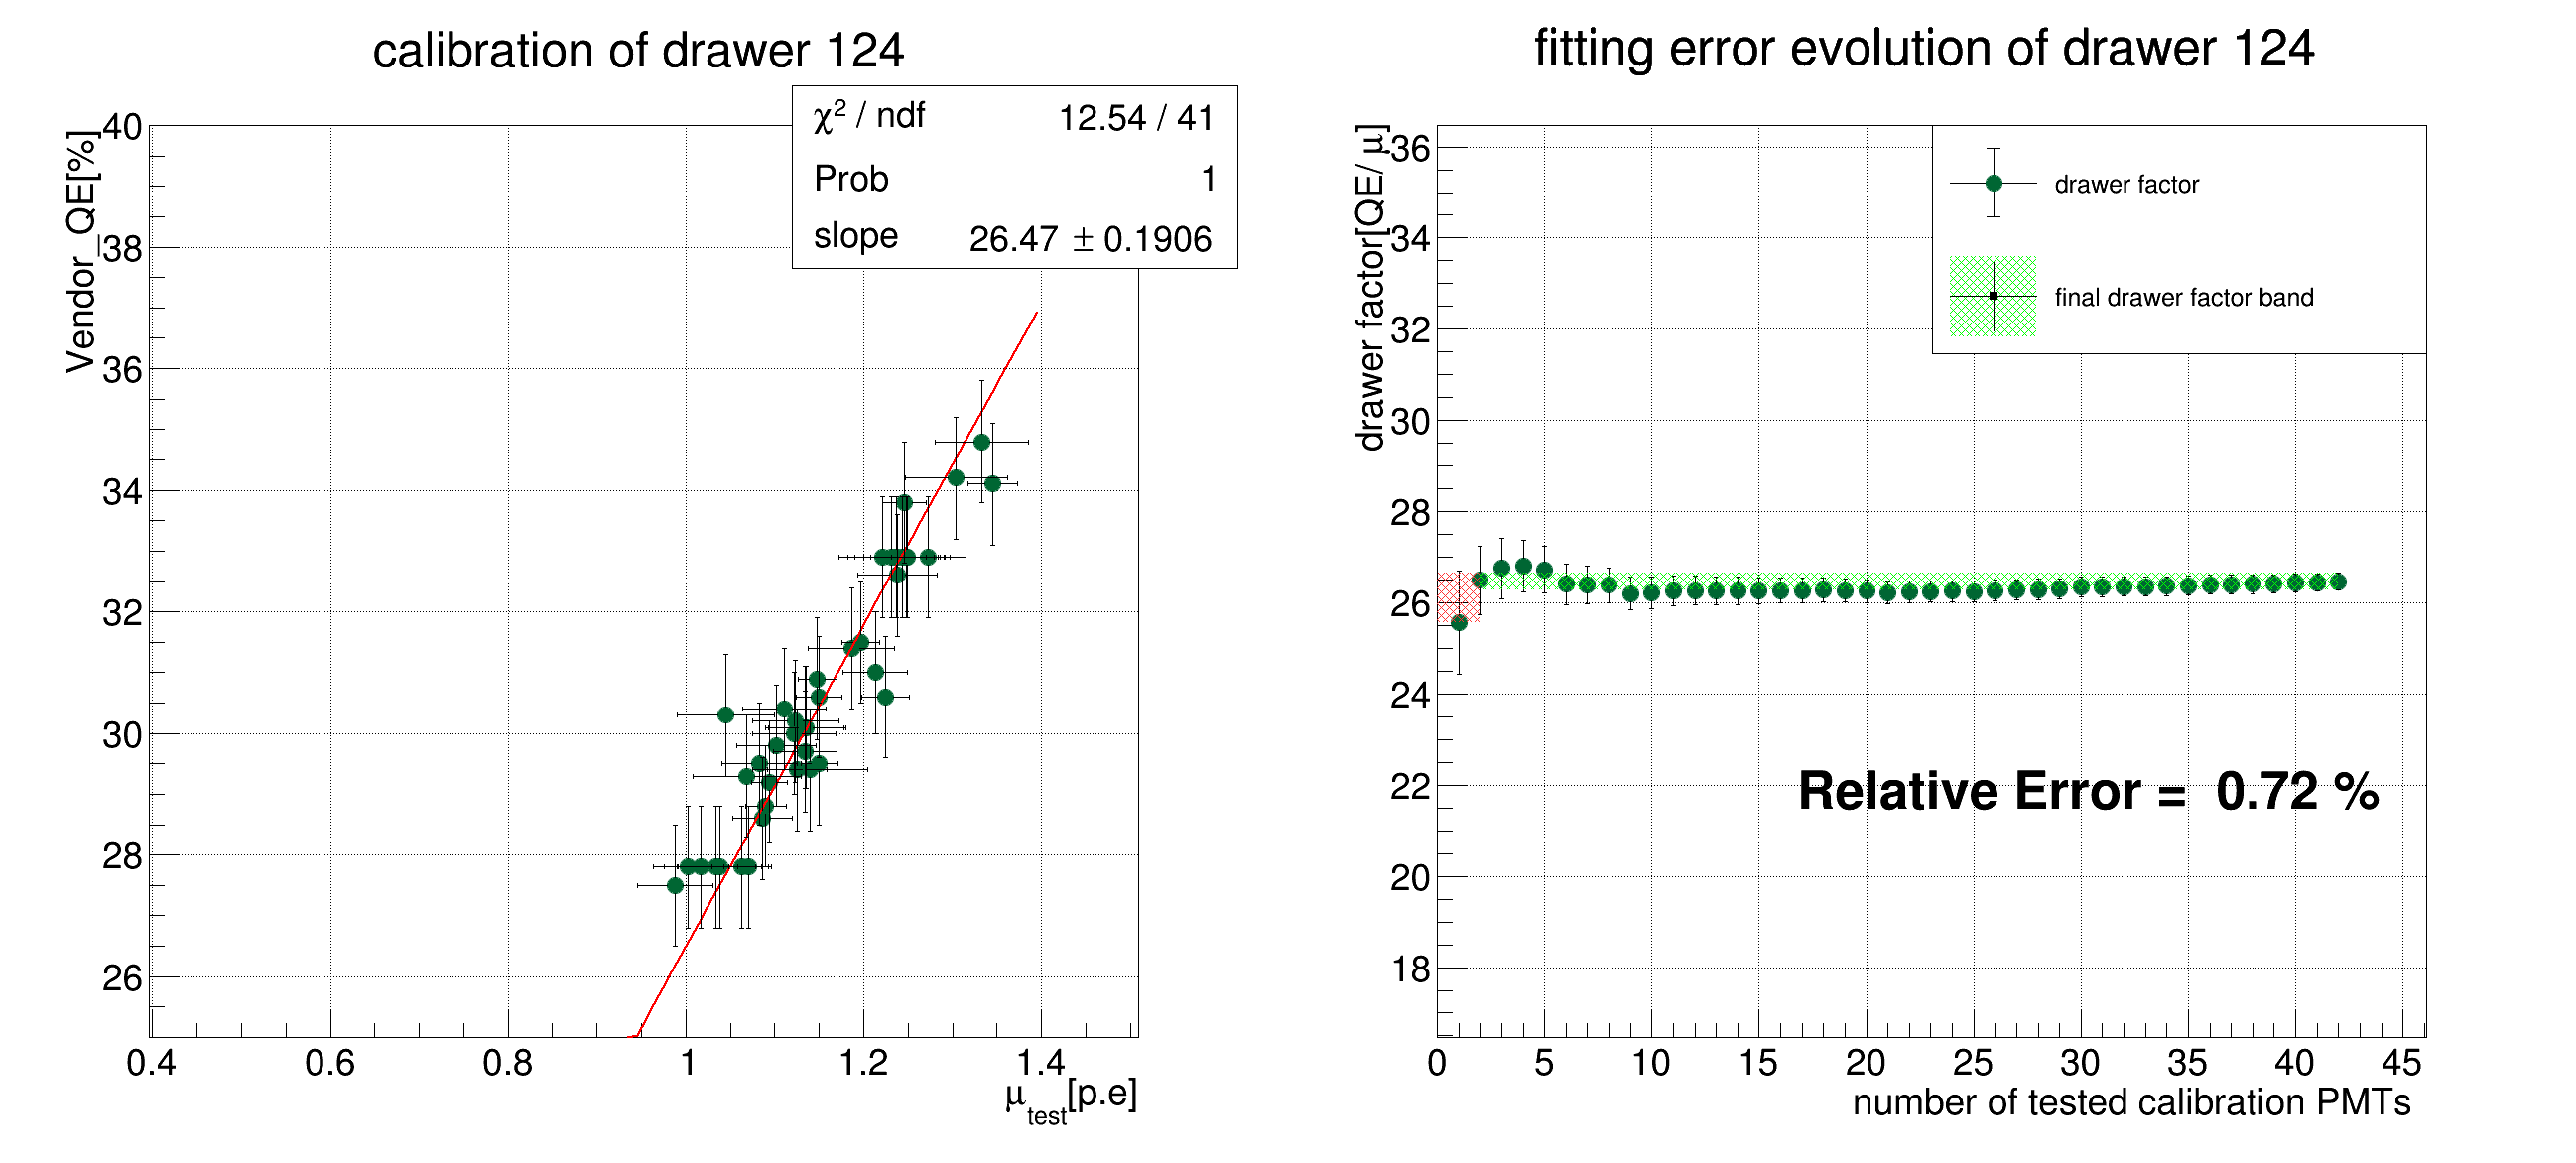
\includegraphics[width=0.45\textwidth]{sta101-23} 
\end{frame}
\begin{frame}{drawer-calibration}
\vspace{-.5cm}
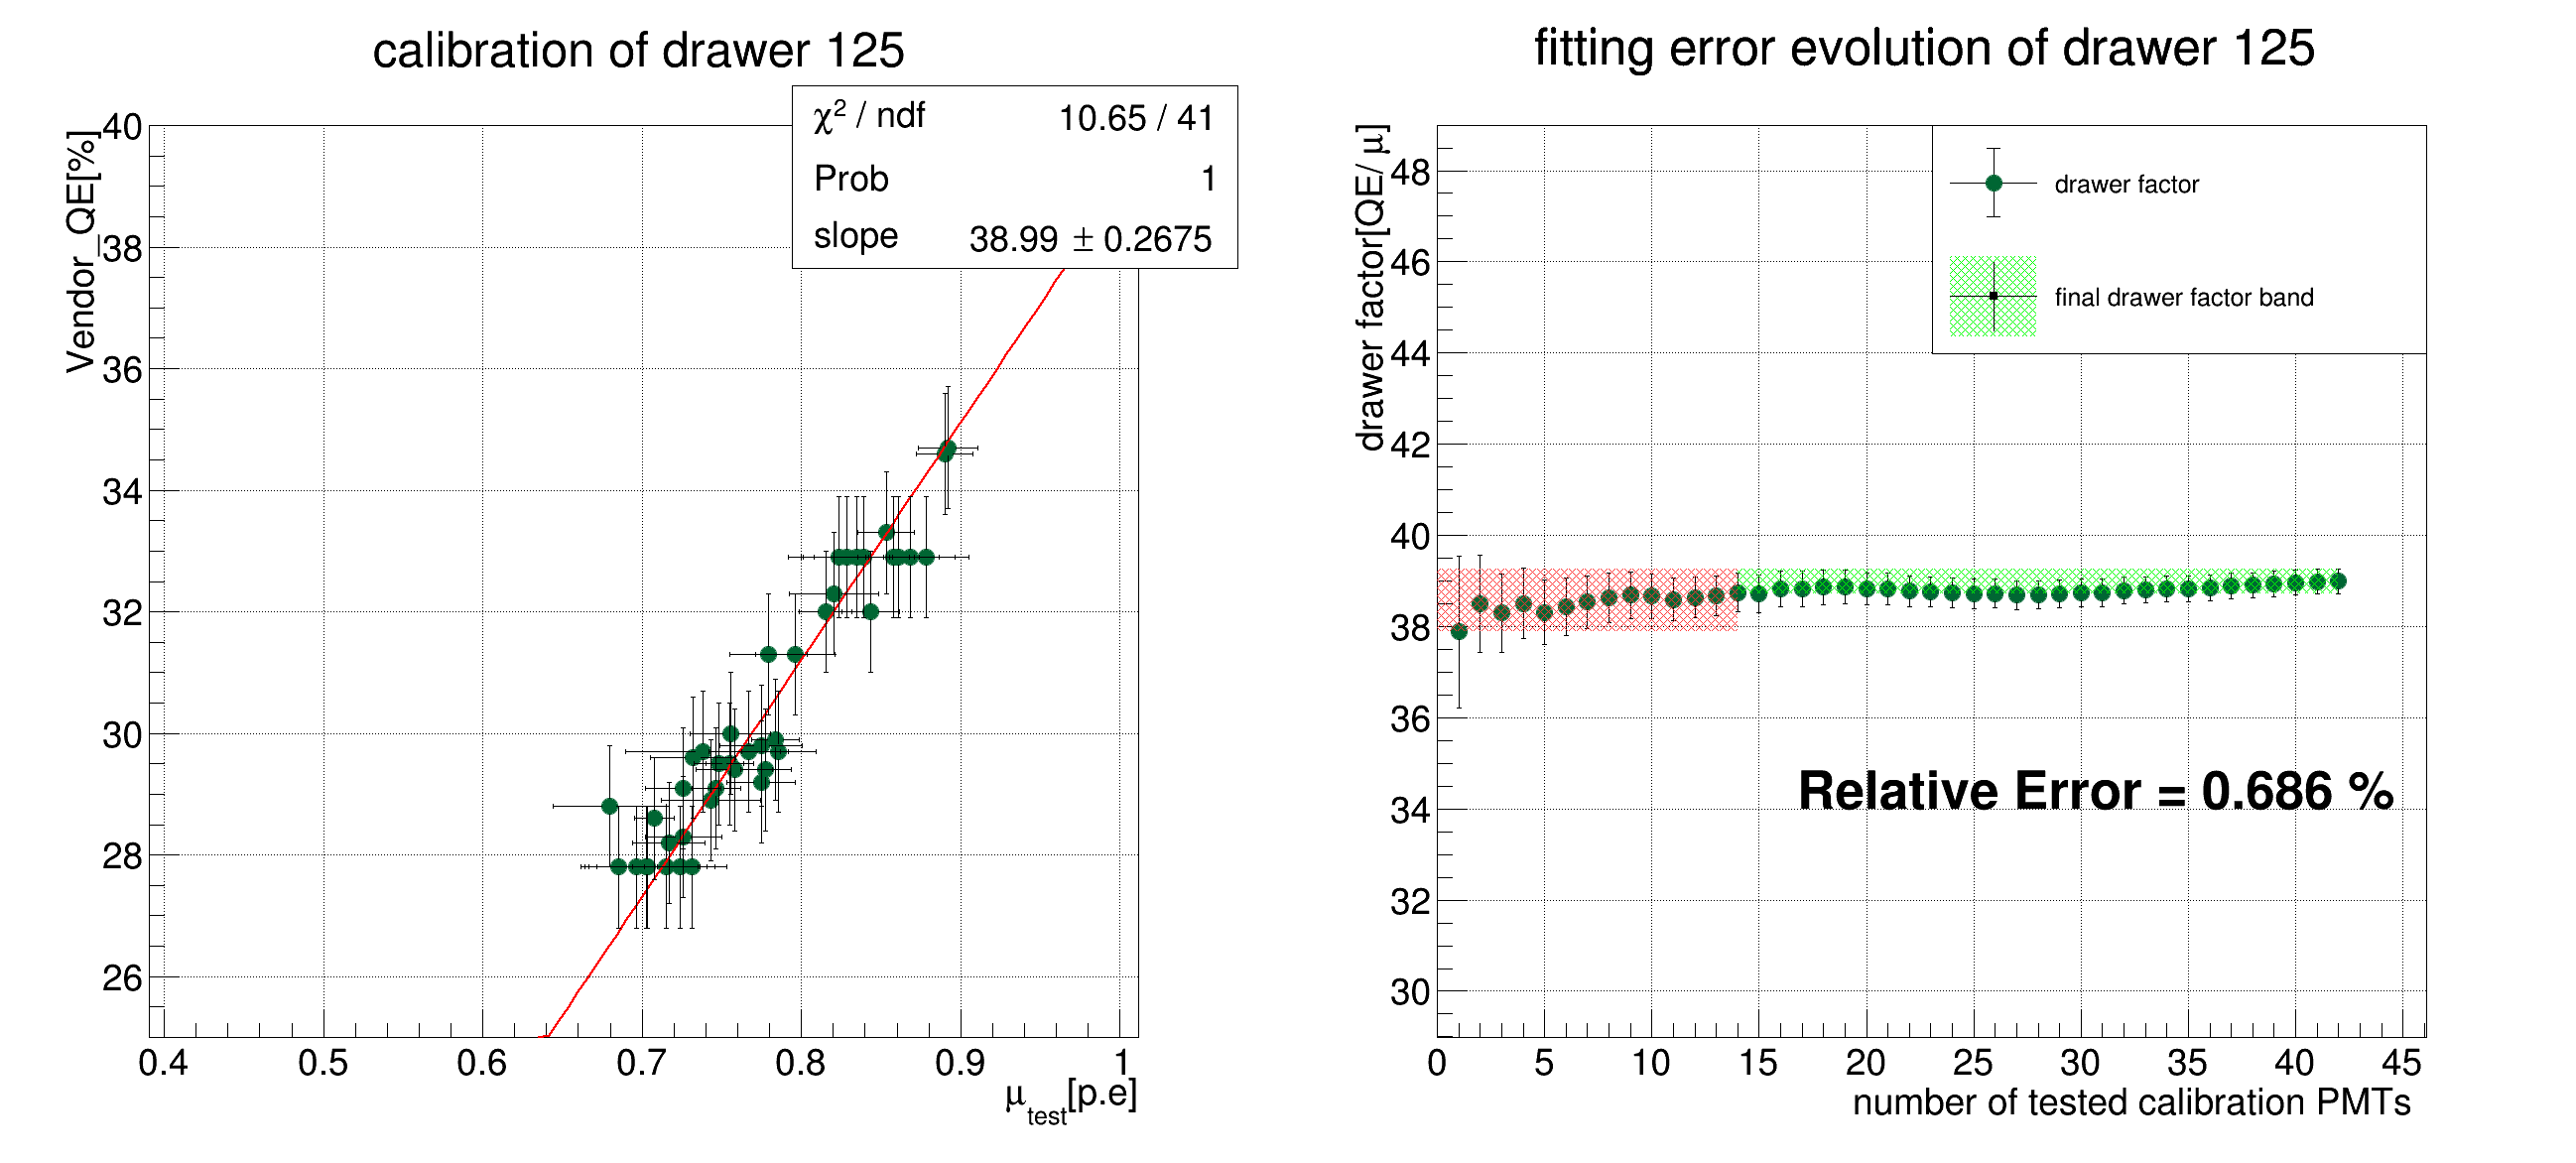
\includegraphics[width=0.45\textwidth]{sta101-24} 
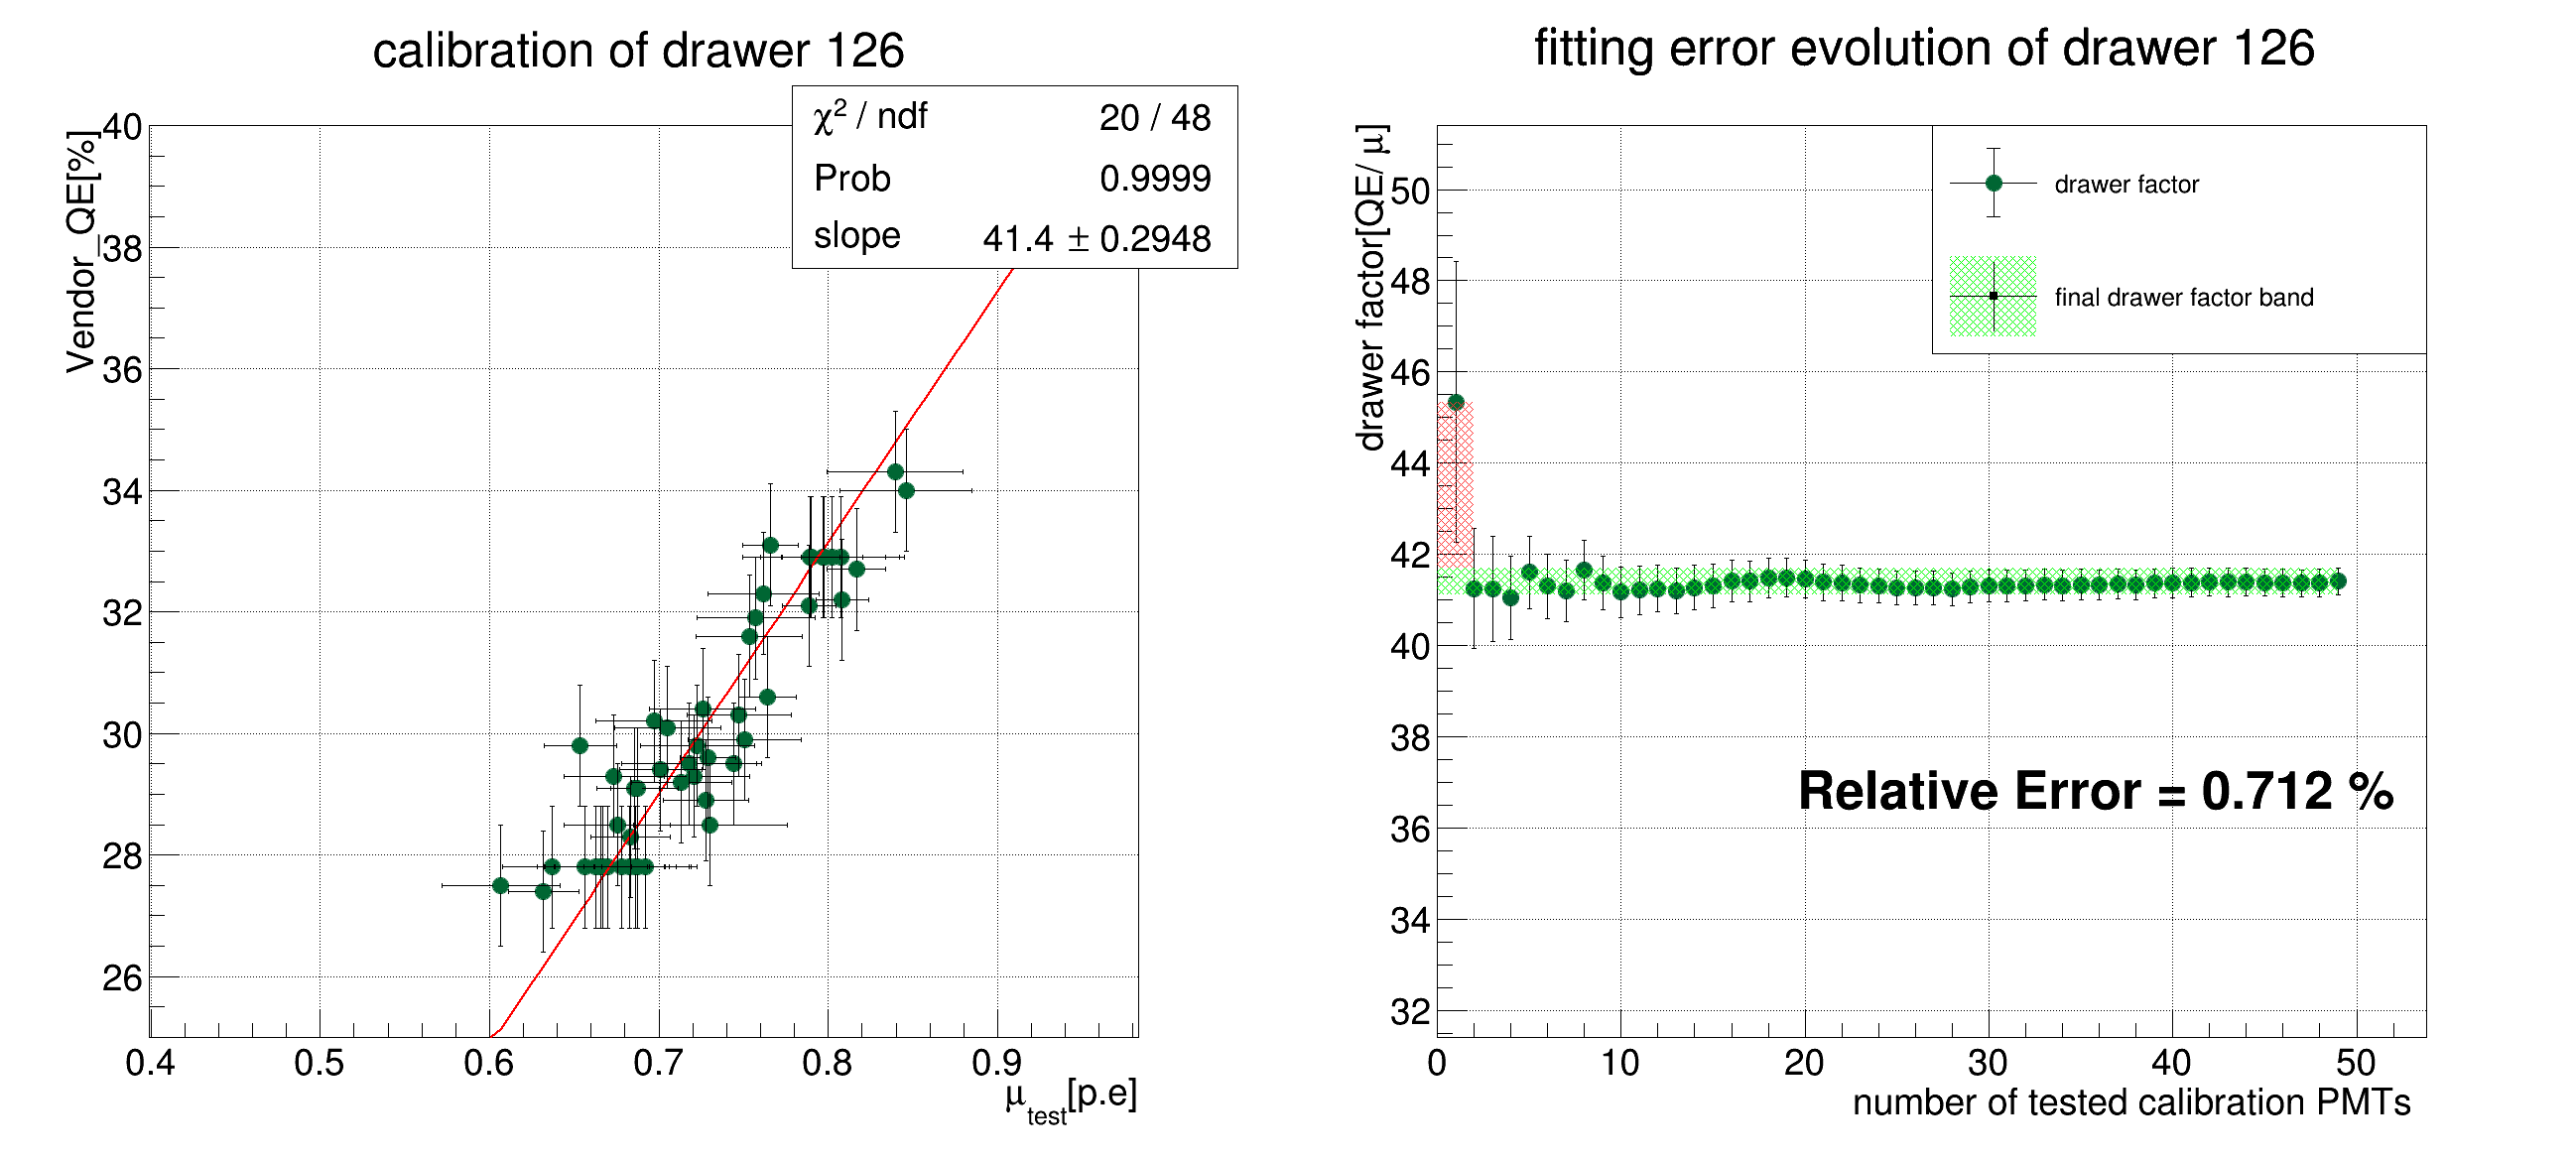
\includegraphics[width=0.45\textwidth]{sta101-25} 
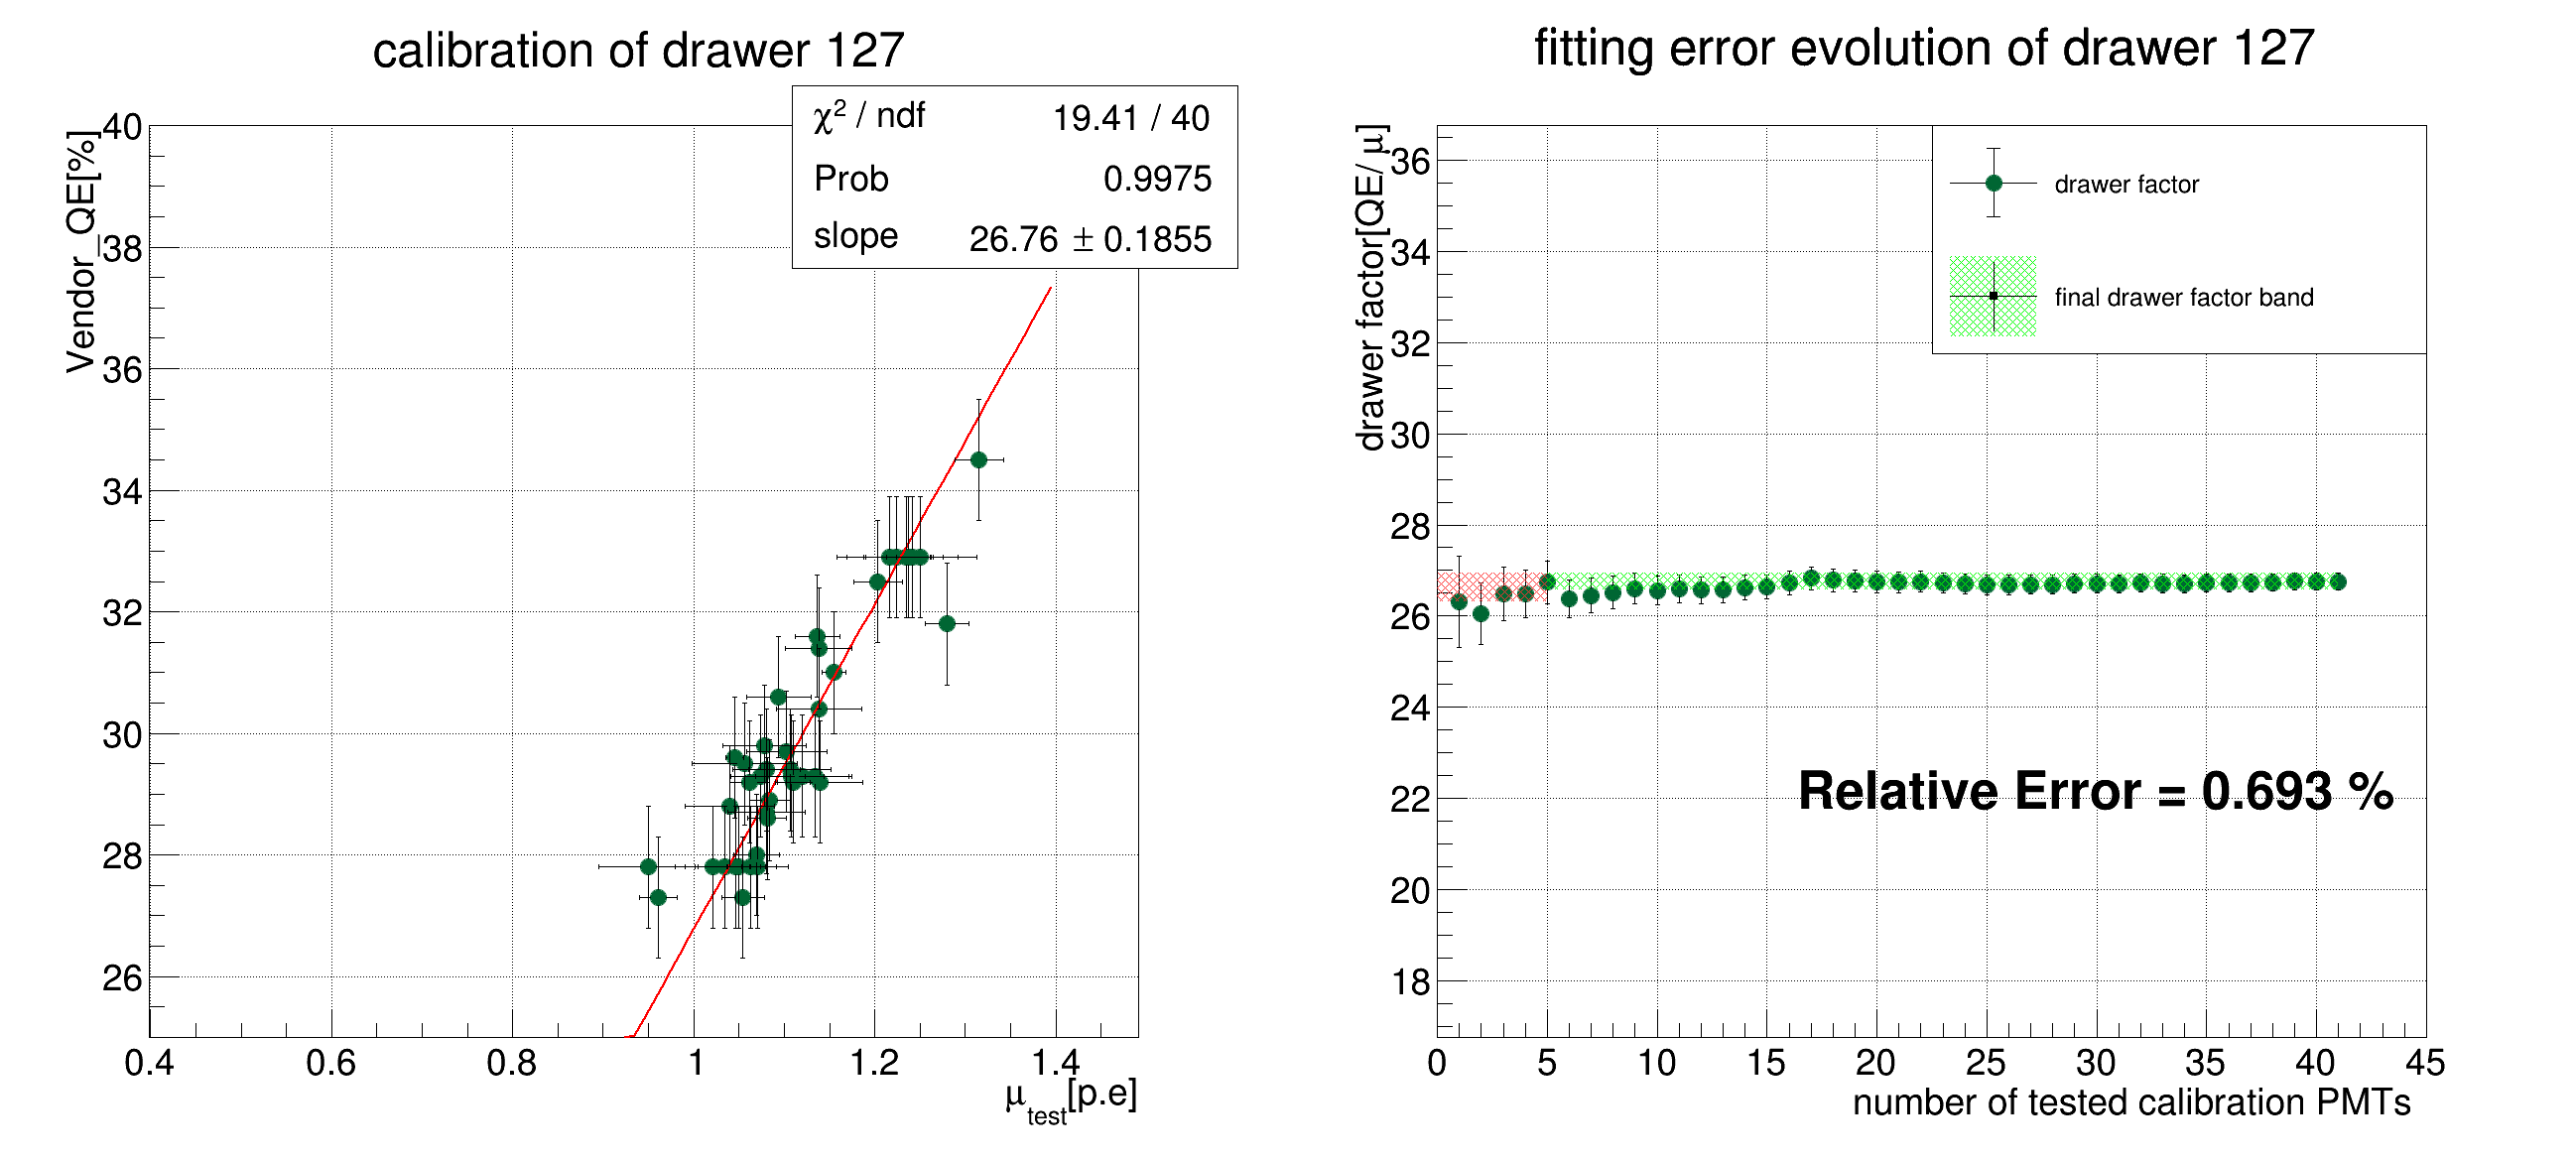
\includegraphics[width=0.45\textwidth]{sta101-26} 
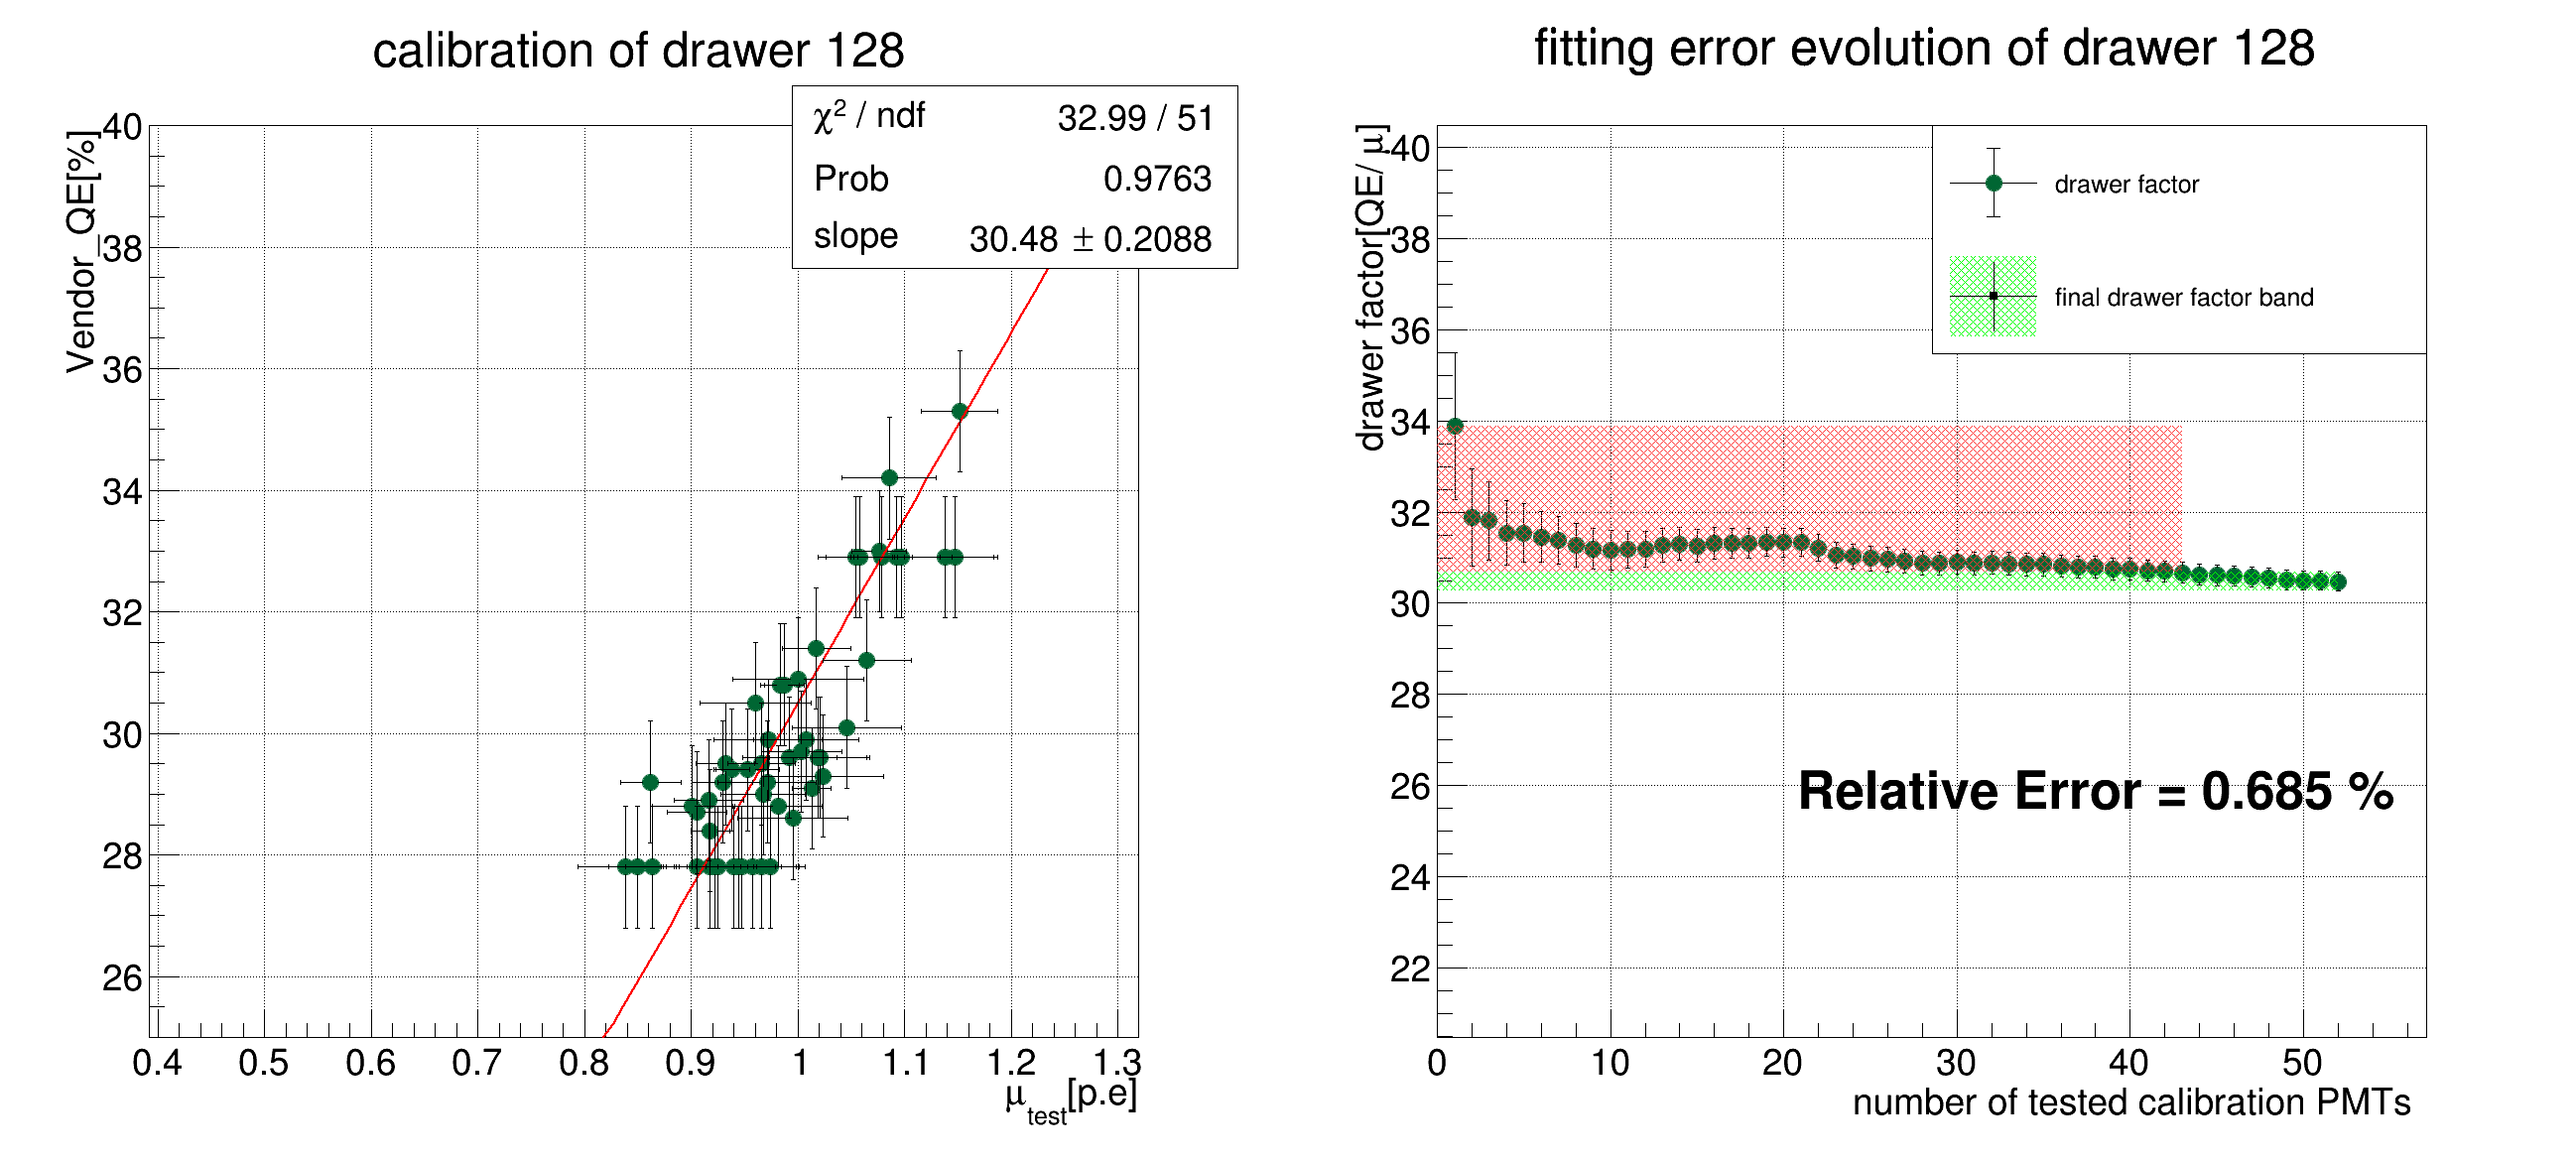
\includegraphics[width=0.45\textwidth]{sta101-27} 
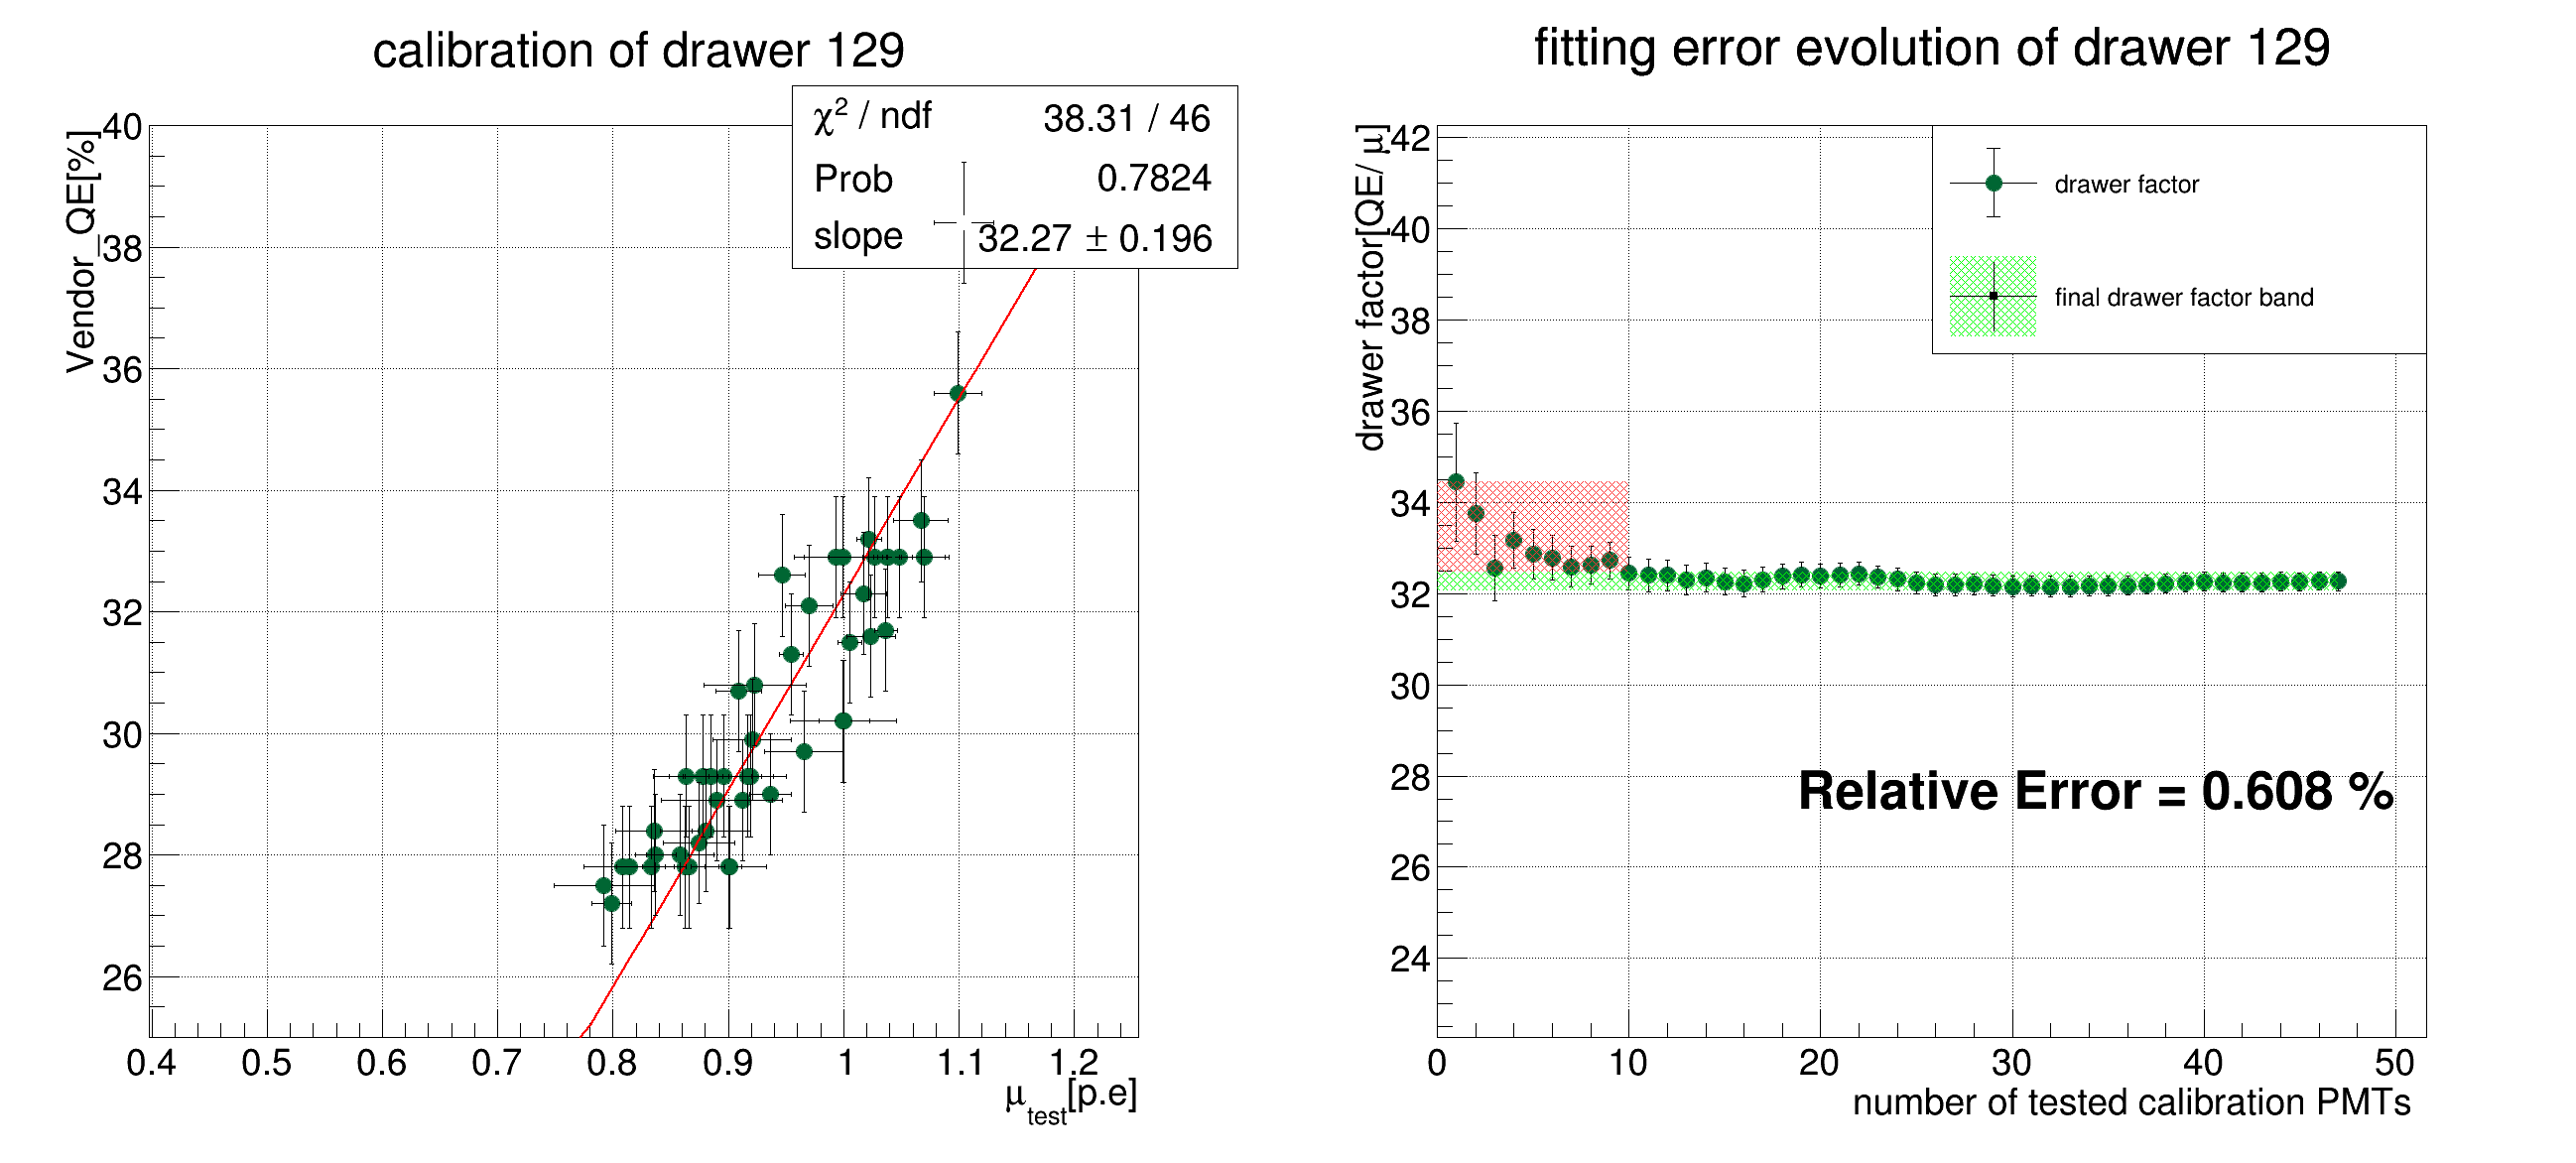
\includegraphics[width=0.45\textwidth]{sta101-28} 
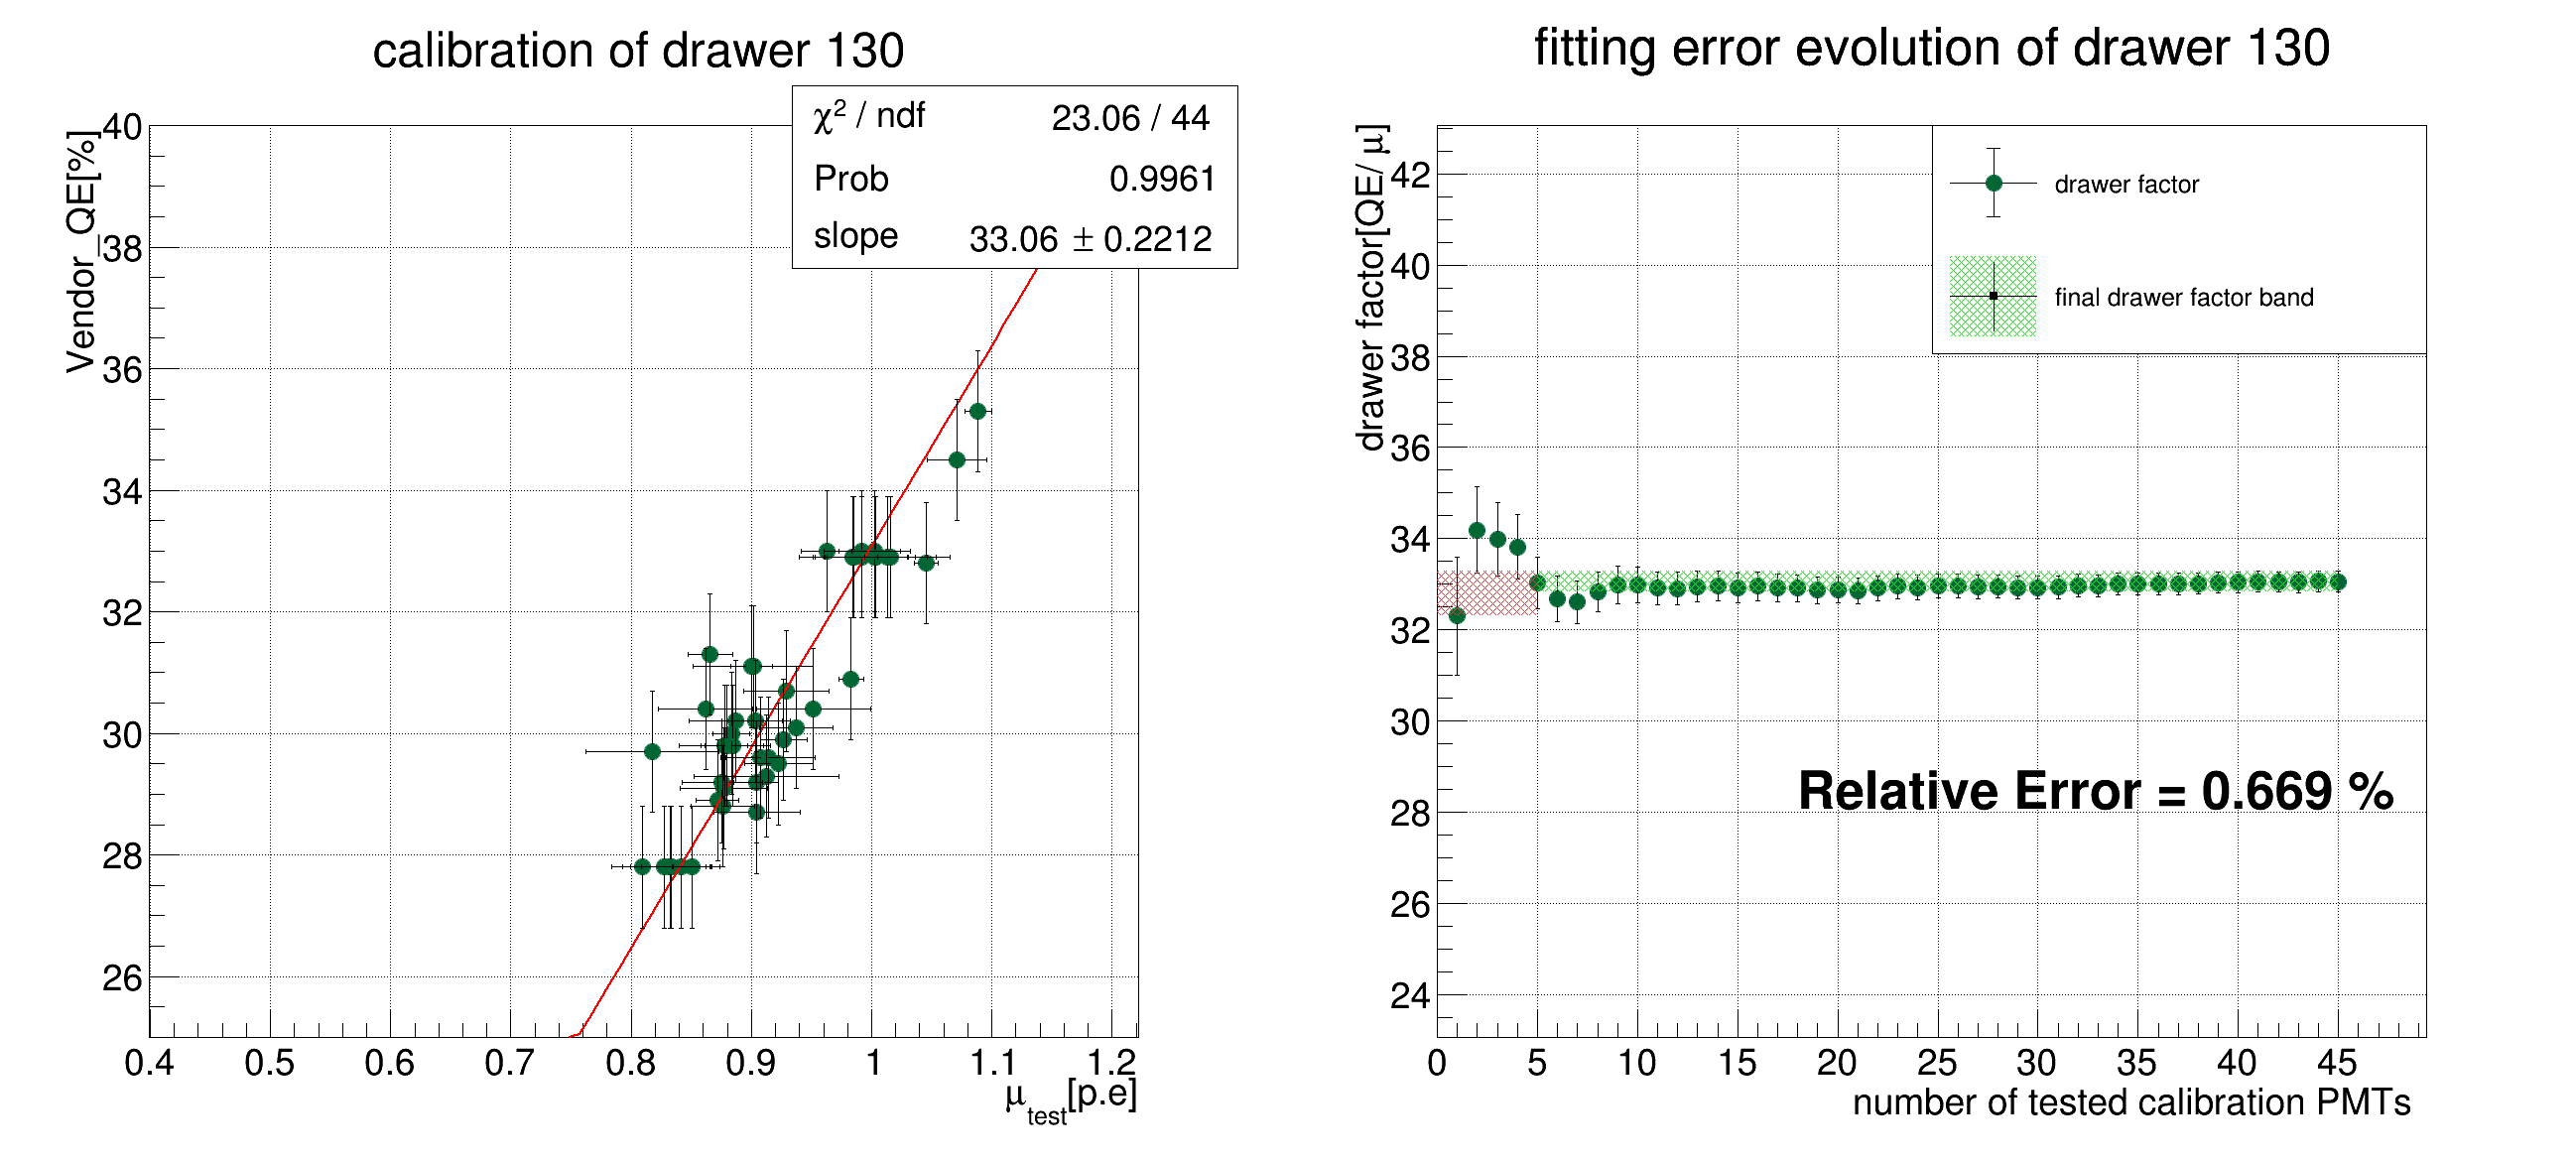
\includegraphics[width=0.45\textwidth]{sta101-29} 
\end{frame}
\begin{frame}{drawer-calibration}
\vspace{-.5cm}
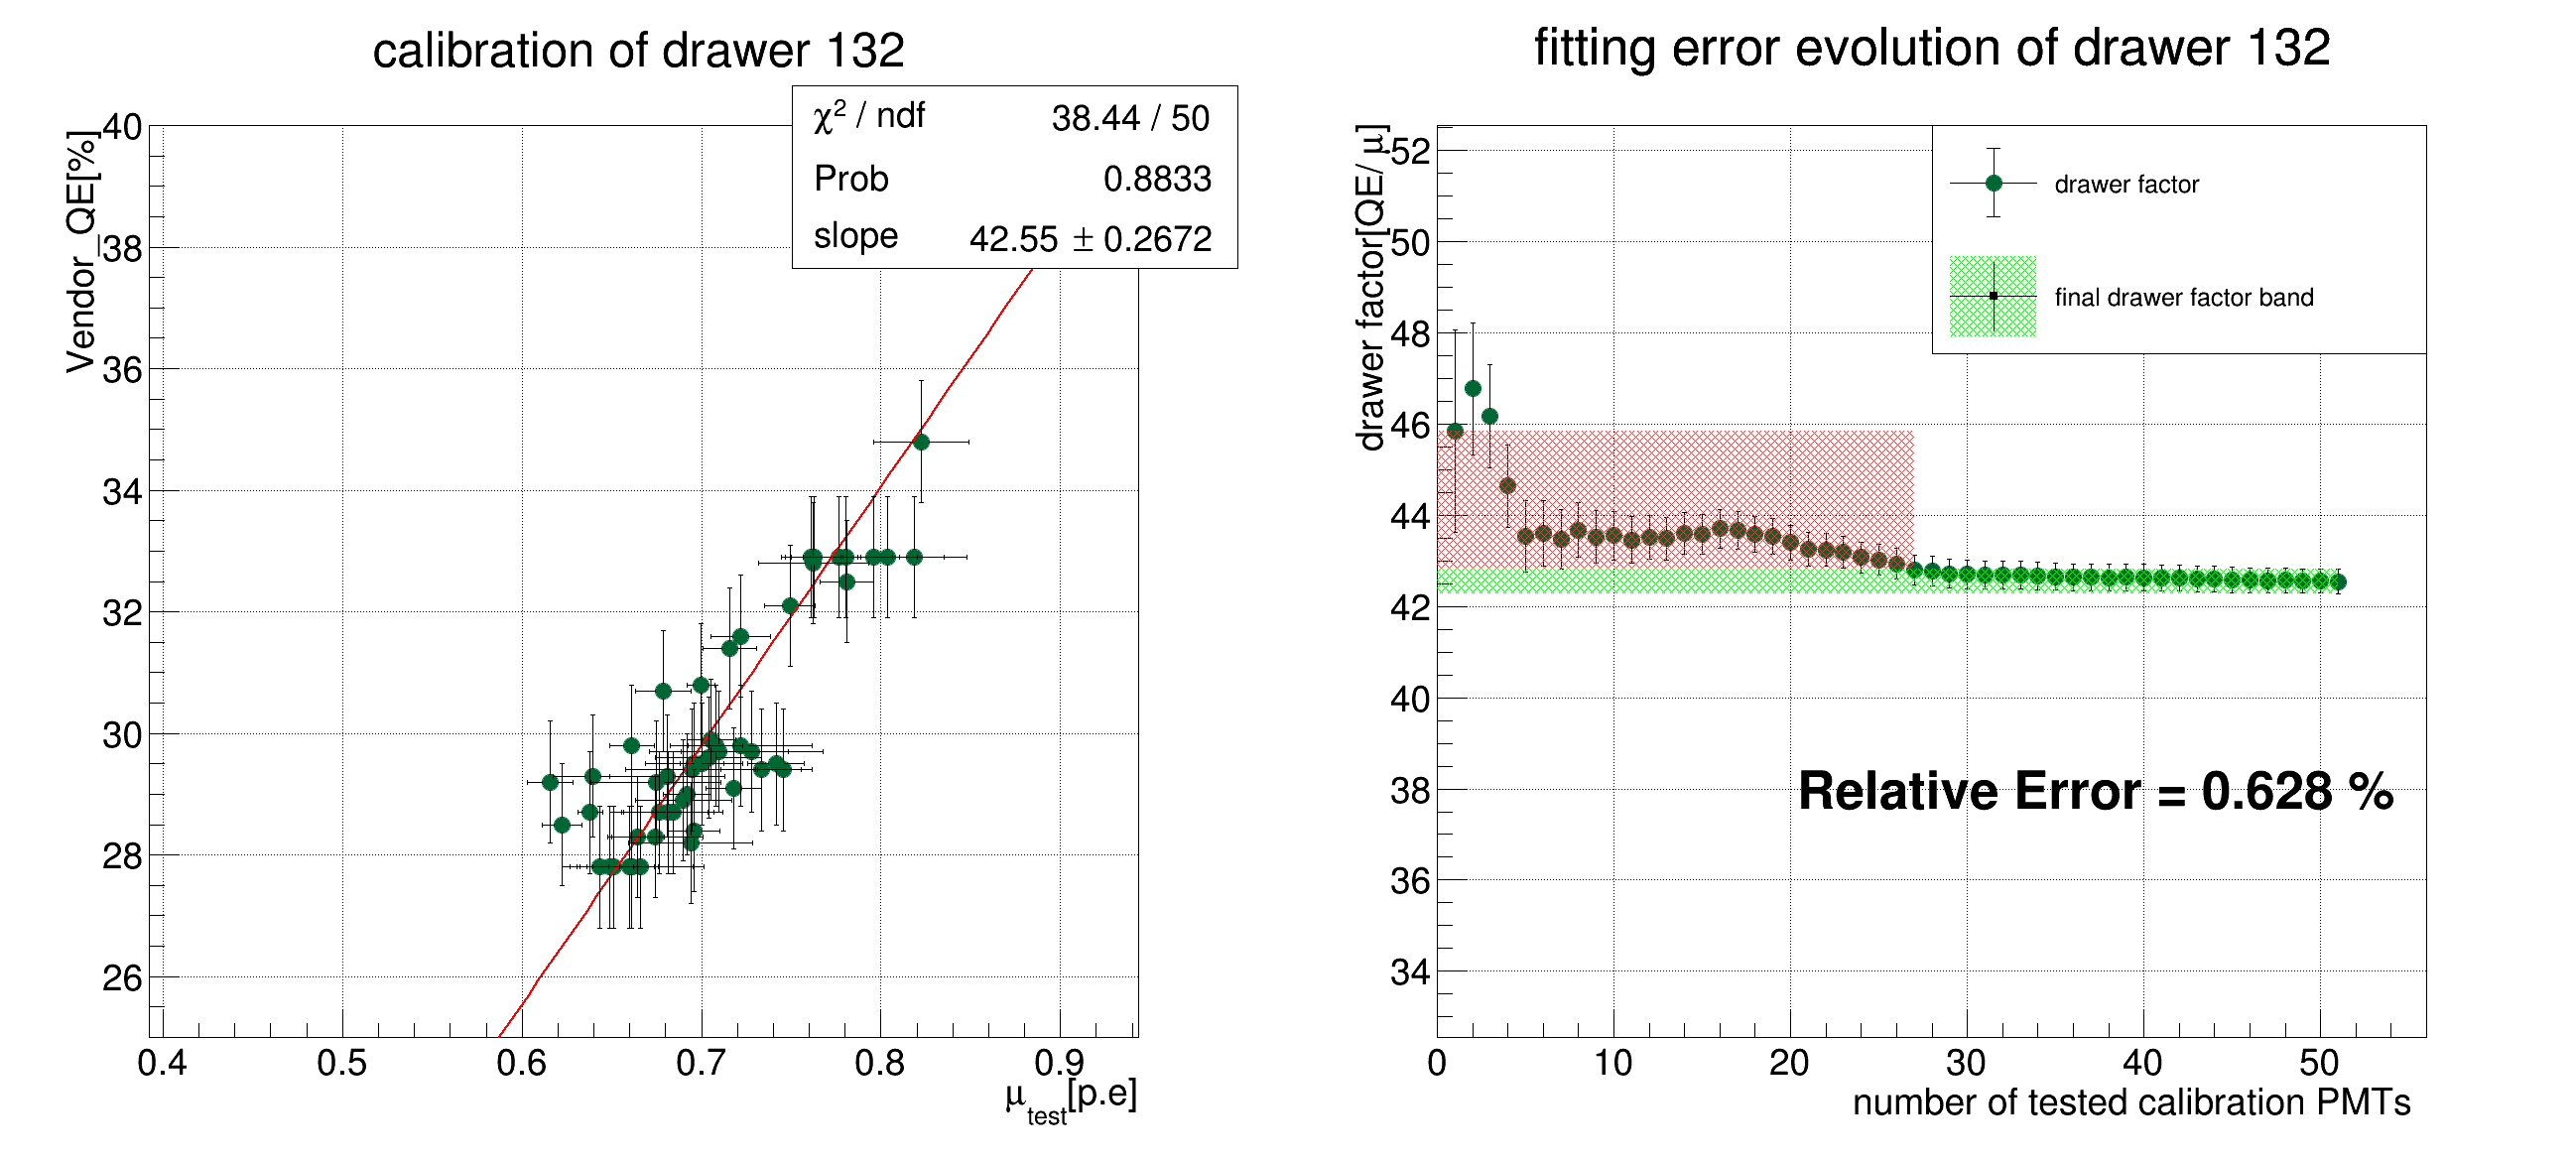
\includegraphics[width=0.45\textwidth]{sta101-30} 
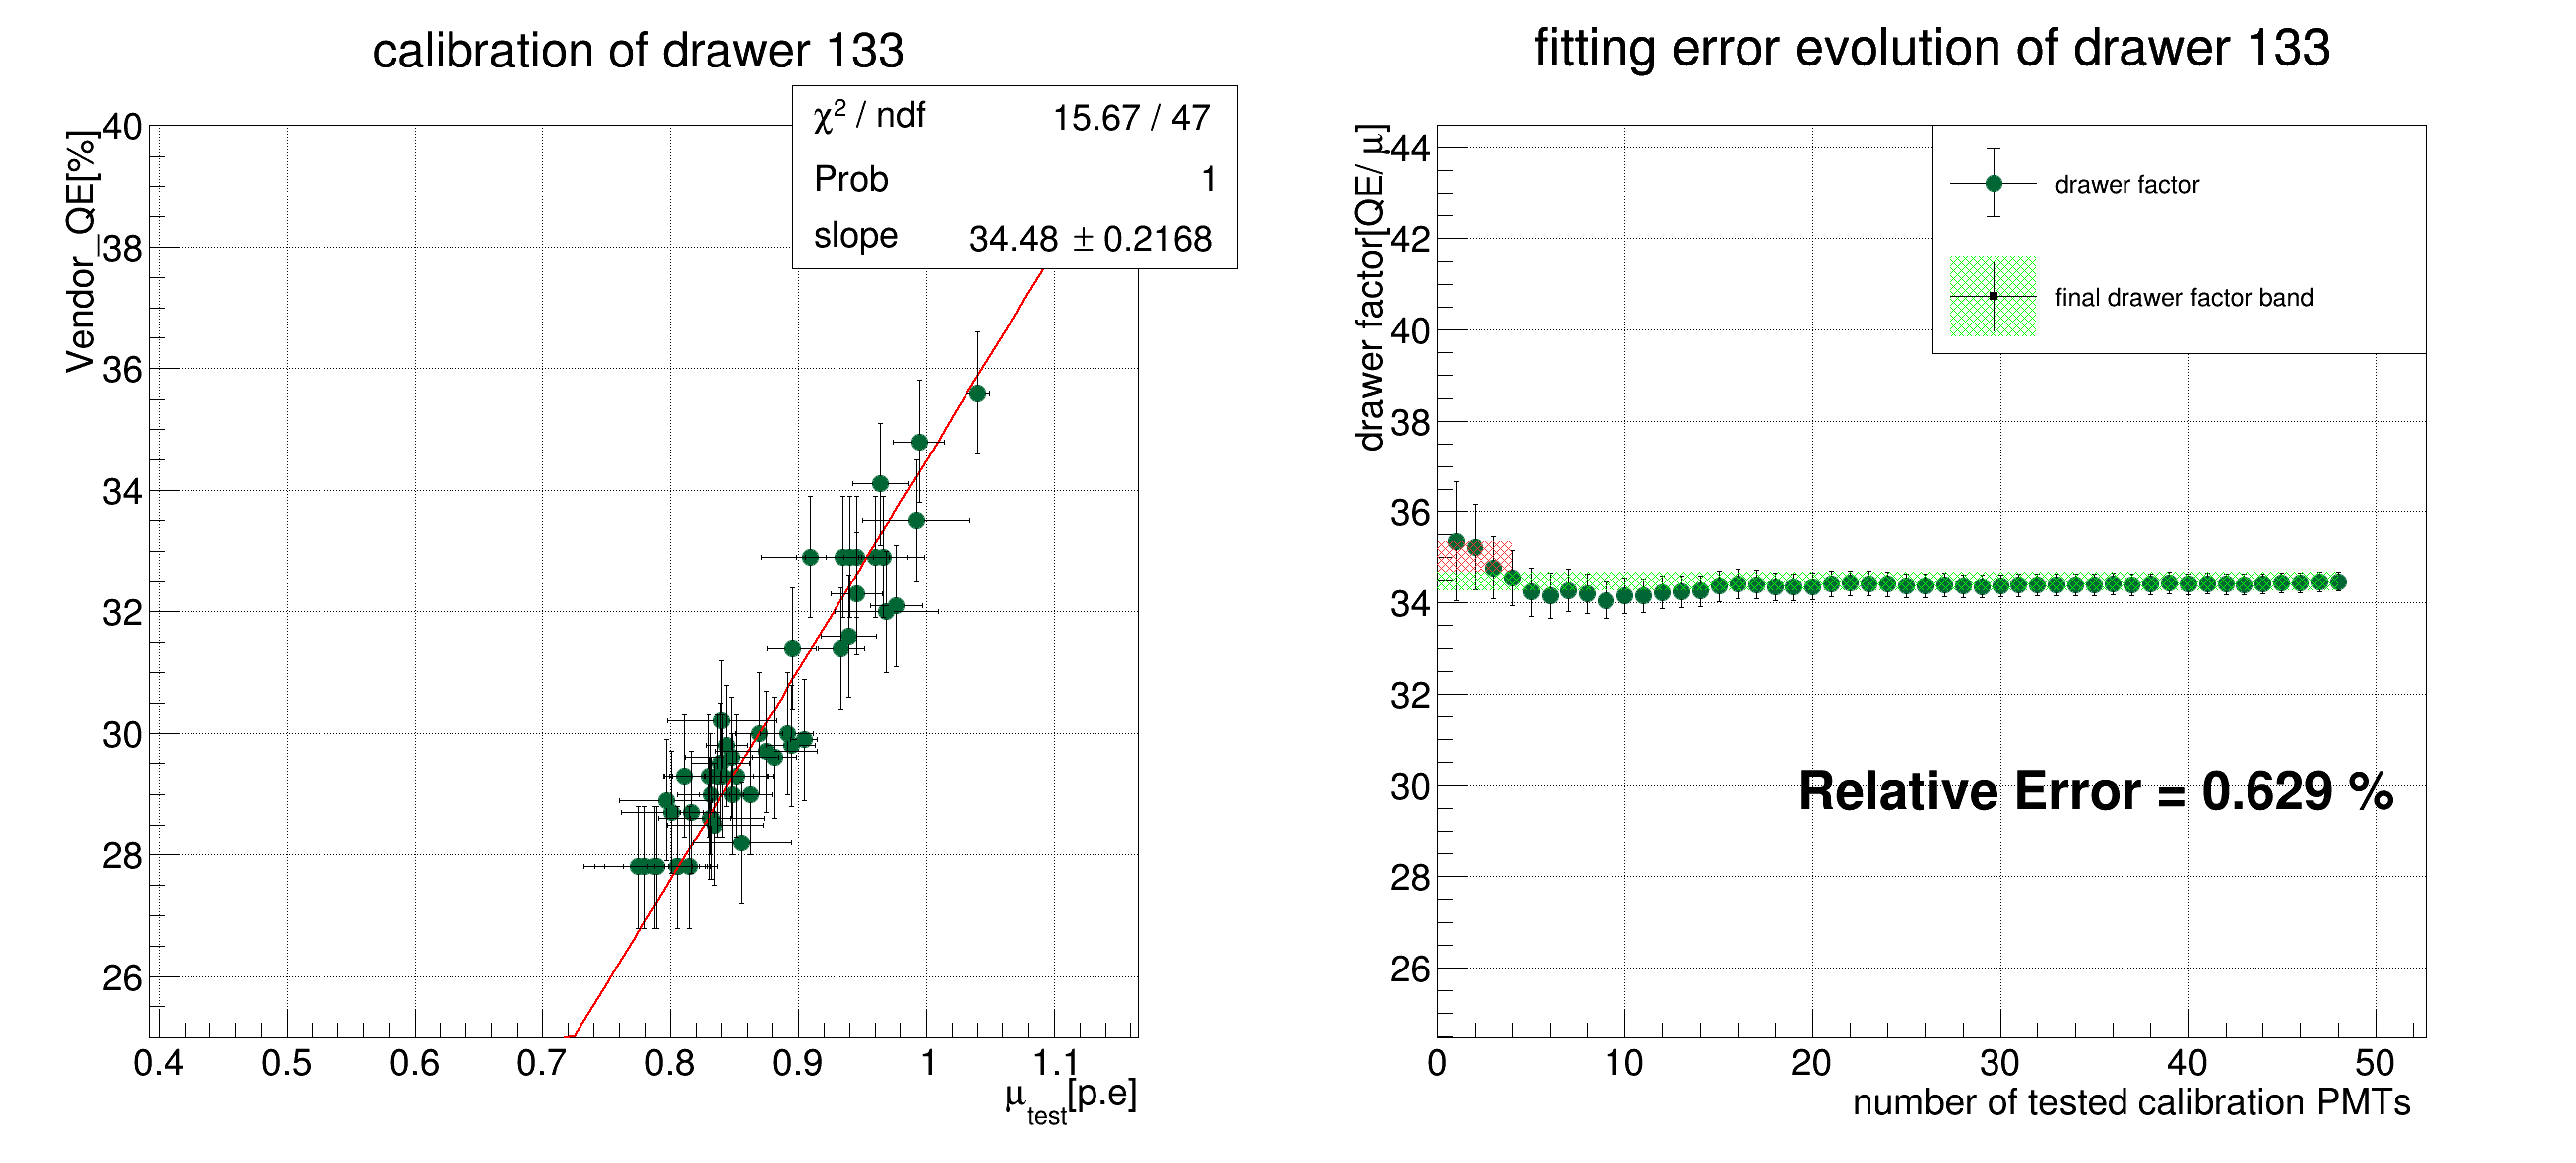
\includegraphics[width=0.45\textwidth]{sta101-31} 
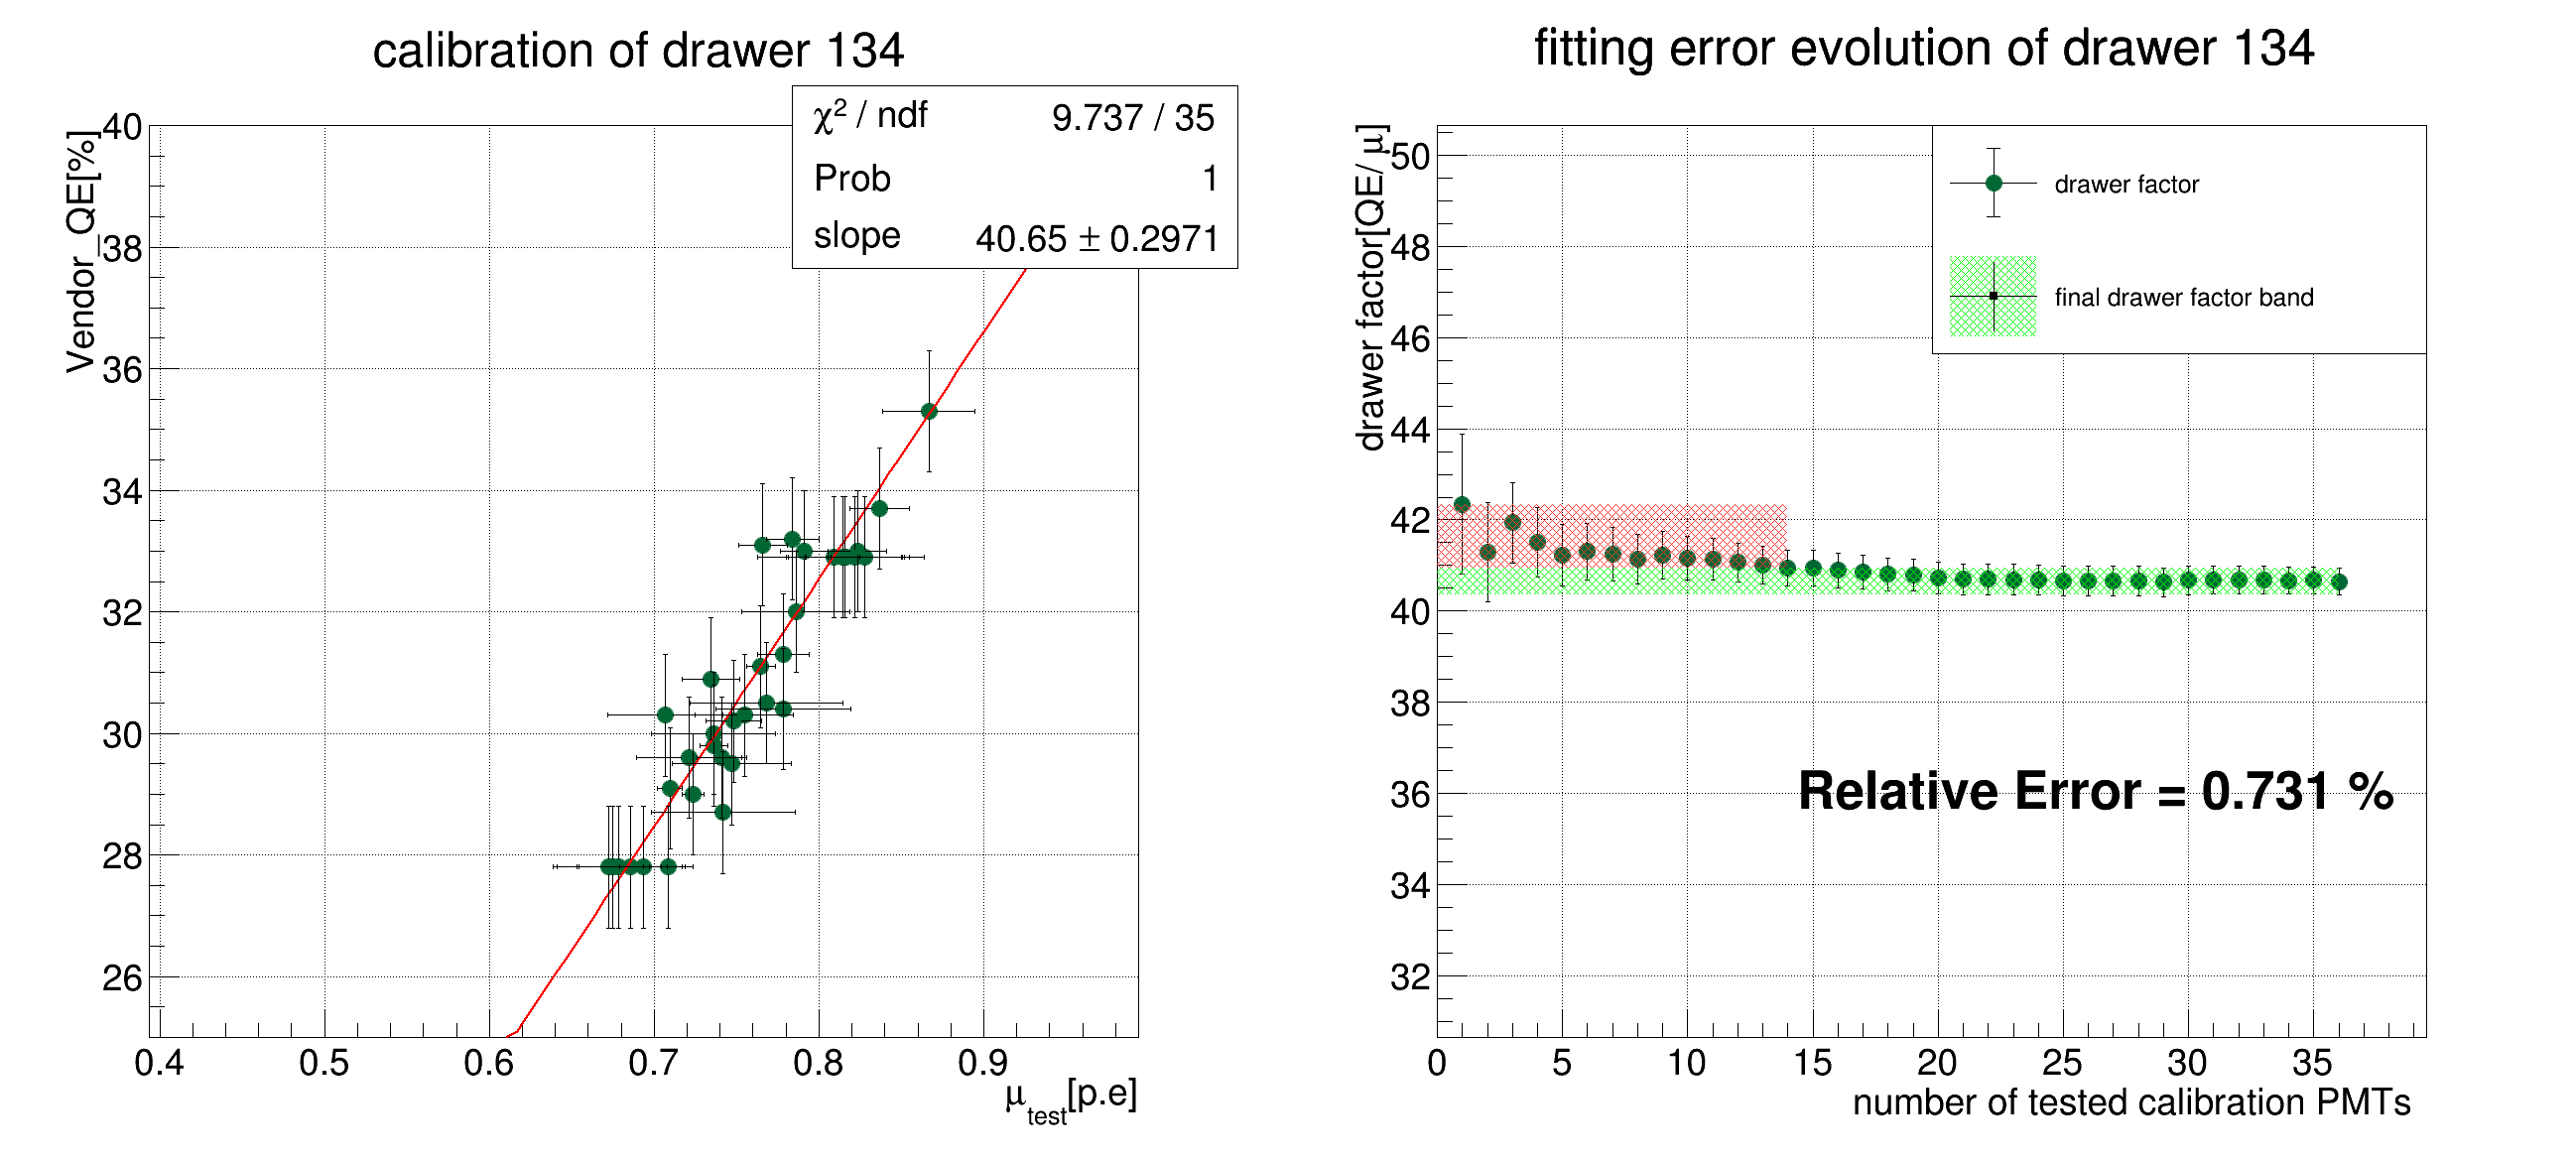
\includegraphics[width=0.45\textwidth]{sta101-32} 
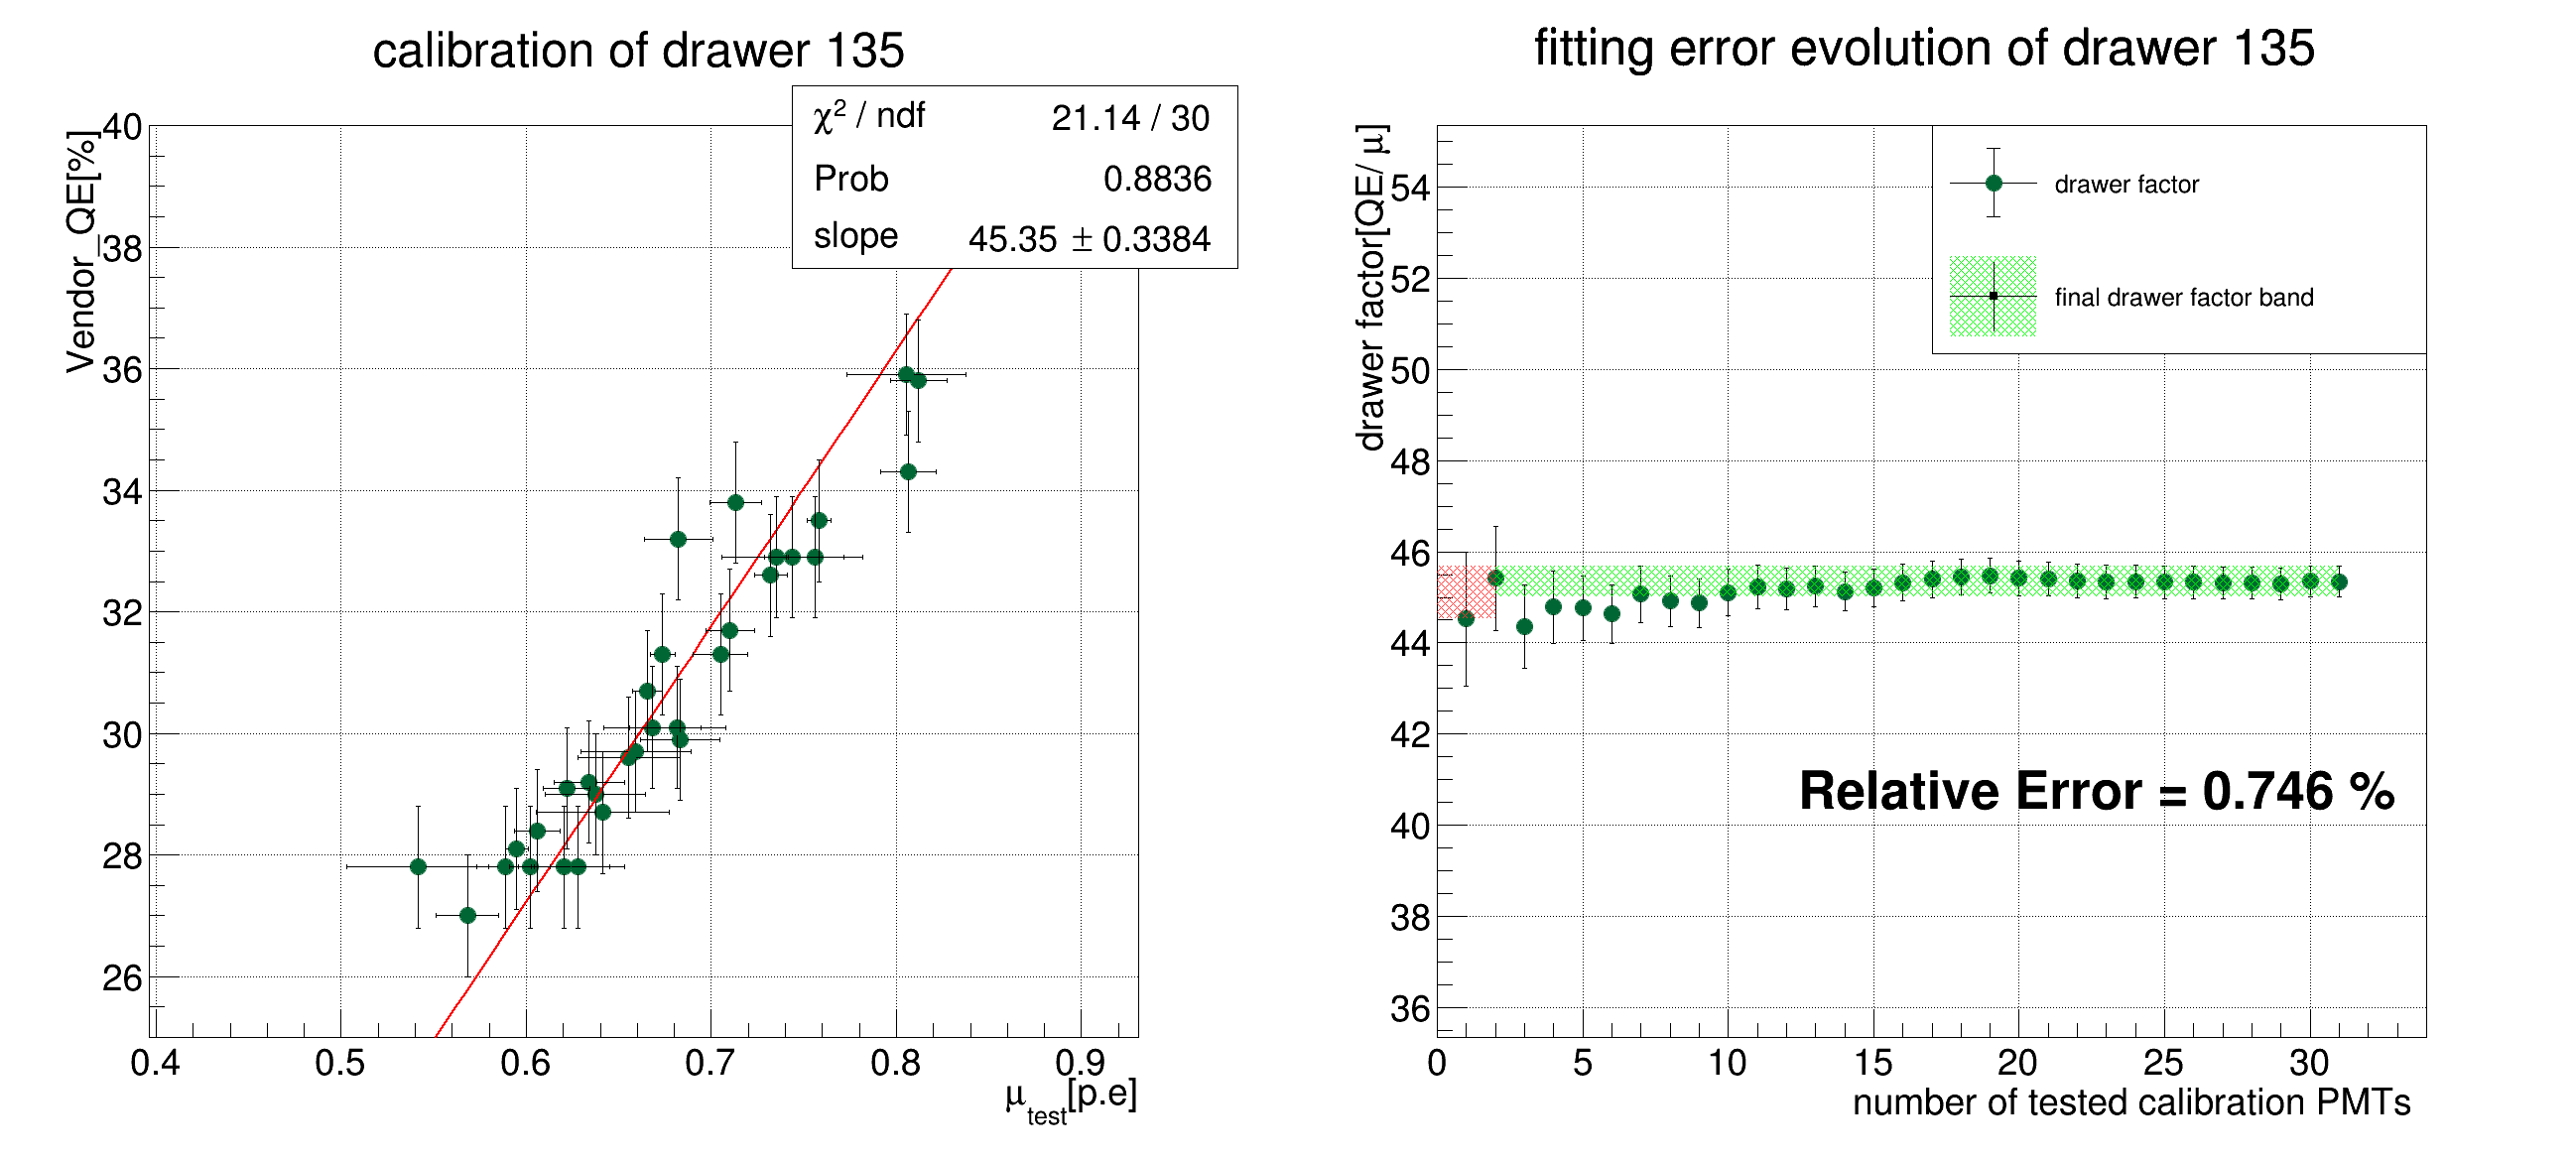
\includegraphics[width=0.45\textwidth]{sta101-33} 
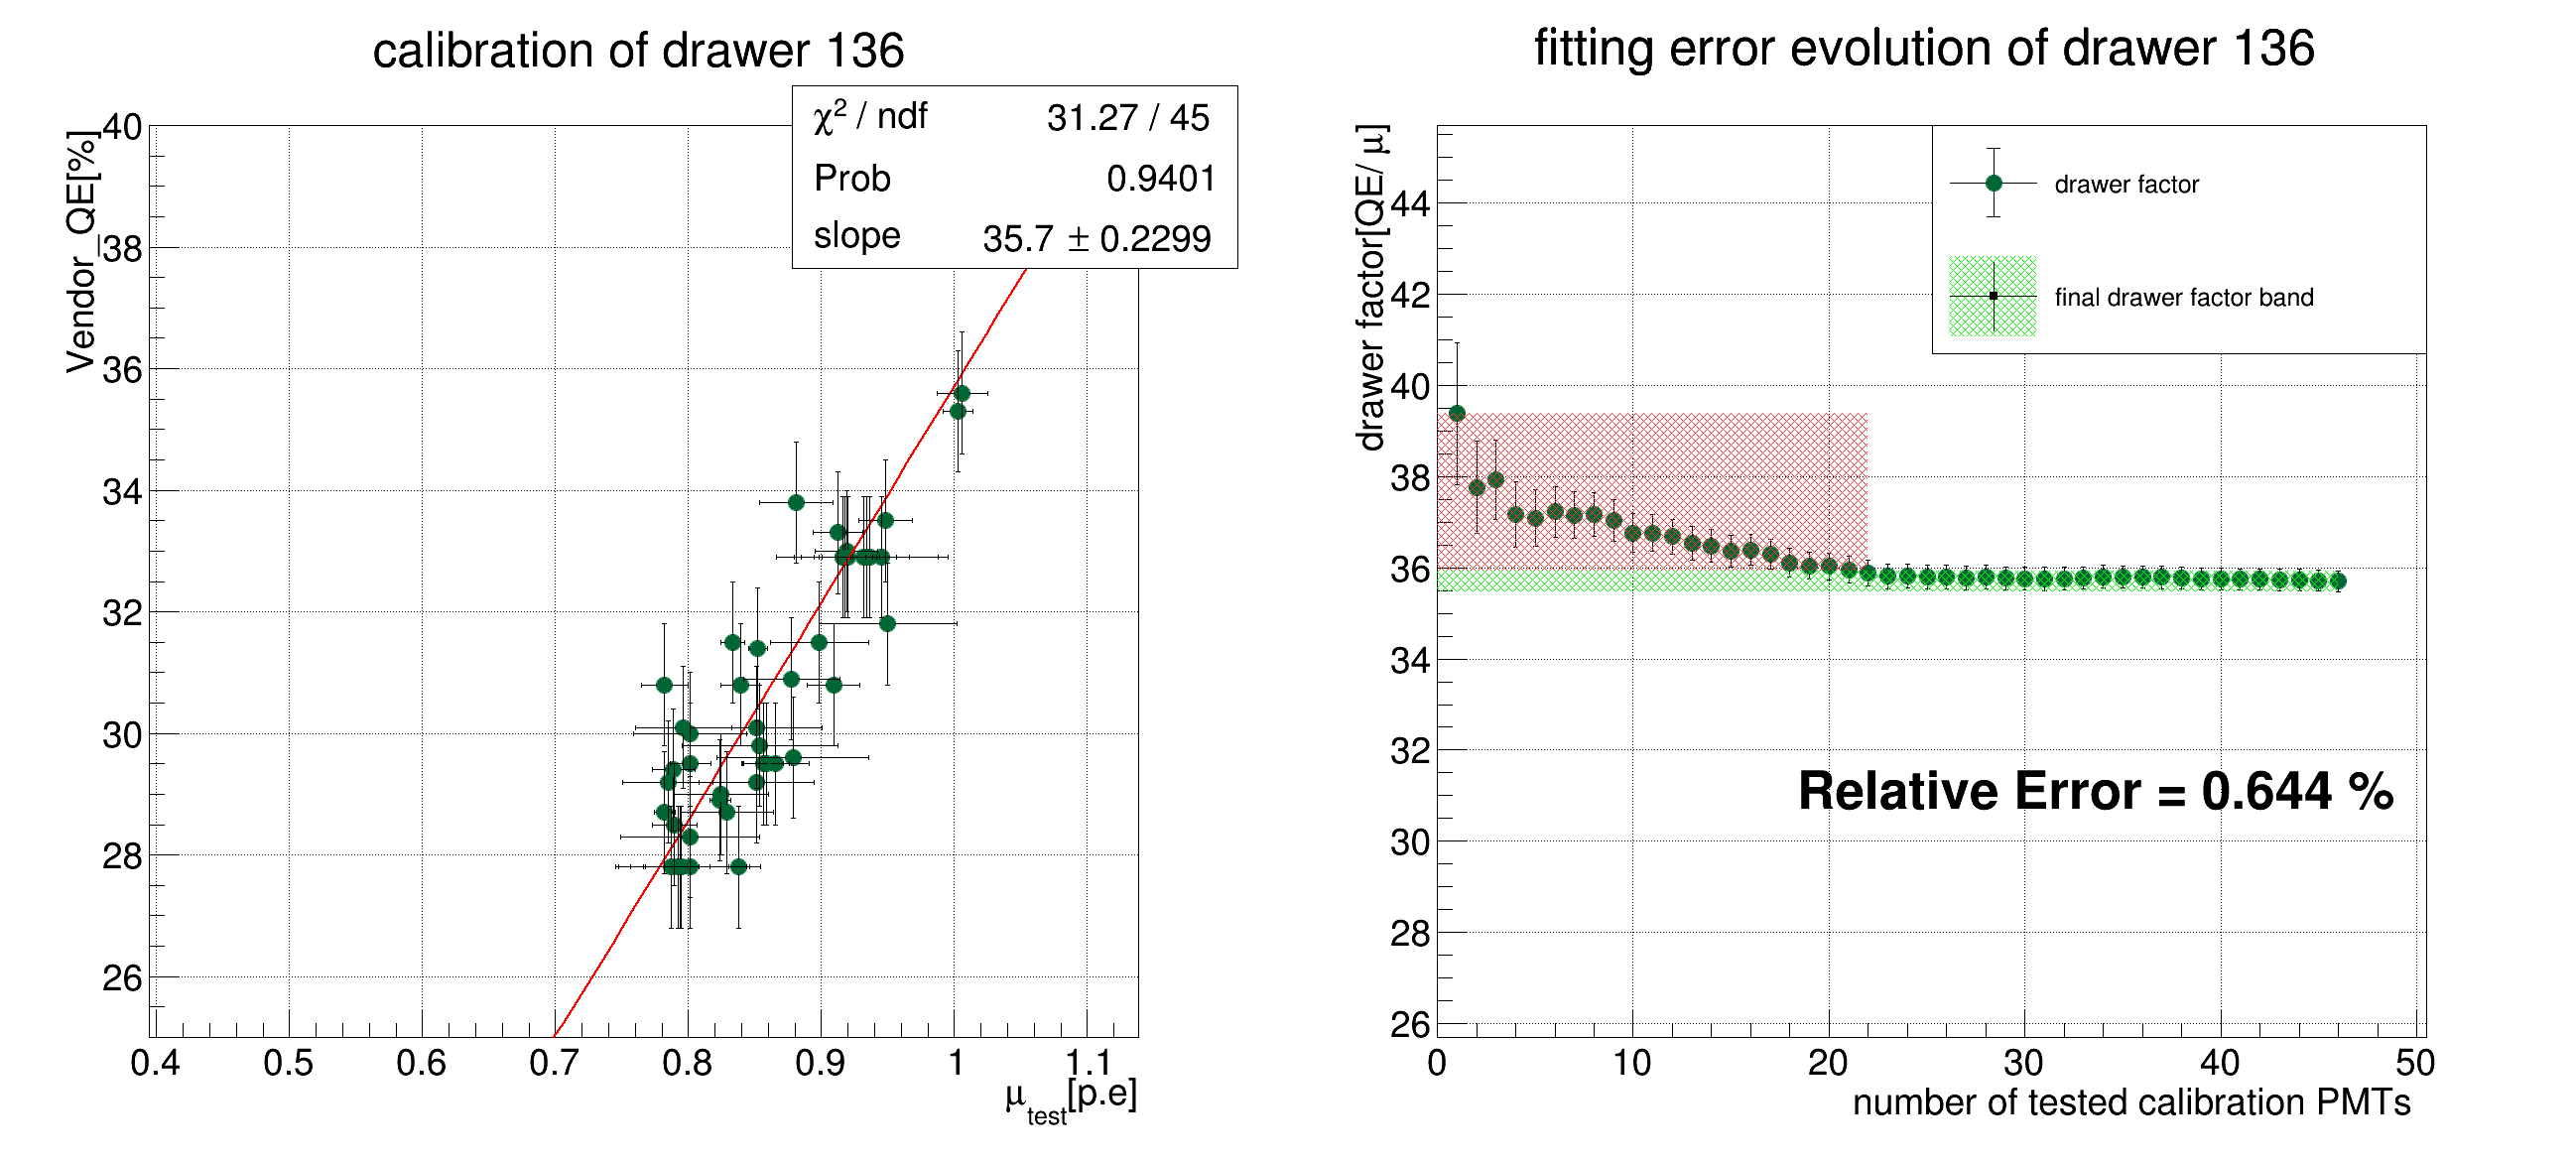
\includegraphics[width=0.45\textwidth]{sta101-34} 
\end{frame}
%%%%%%%%%%%%%%%%%%%%%%%%%%%%%%%%%%%%%%%%%
\begin{frame}{抽屉因子的比较}
factor\_1是我的结果,factor\_2是张海琼的结果。$y=1.148x+0.998$
\vspace{-.05cm}
\begin{figure}
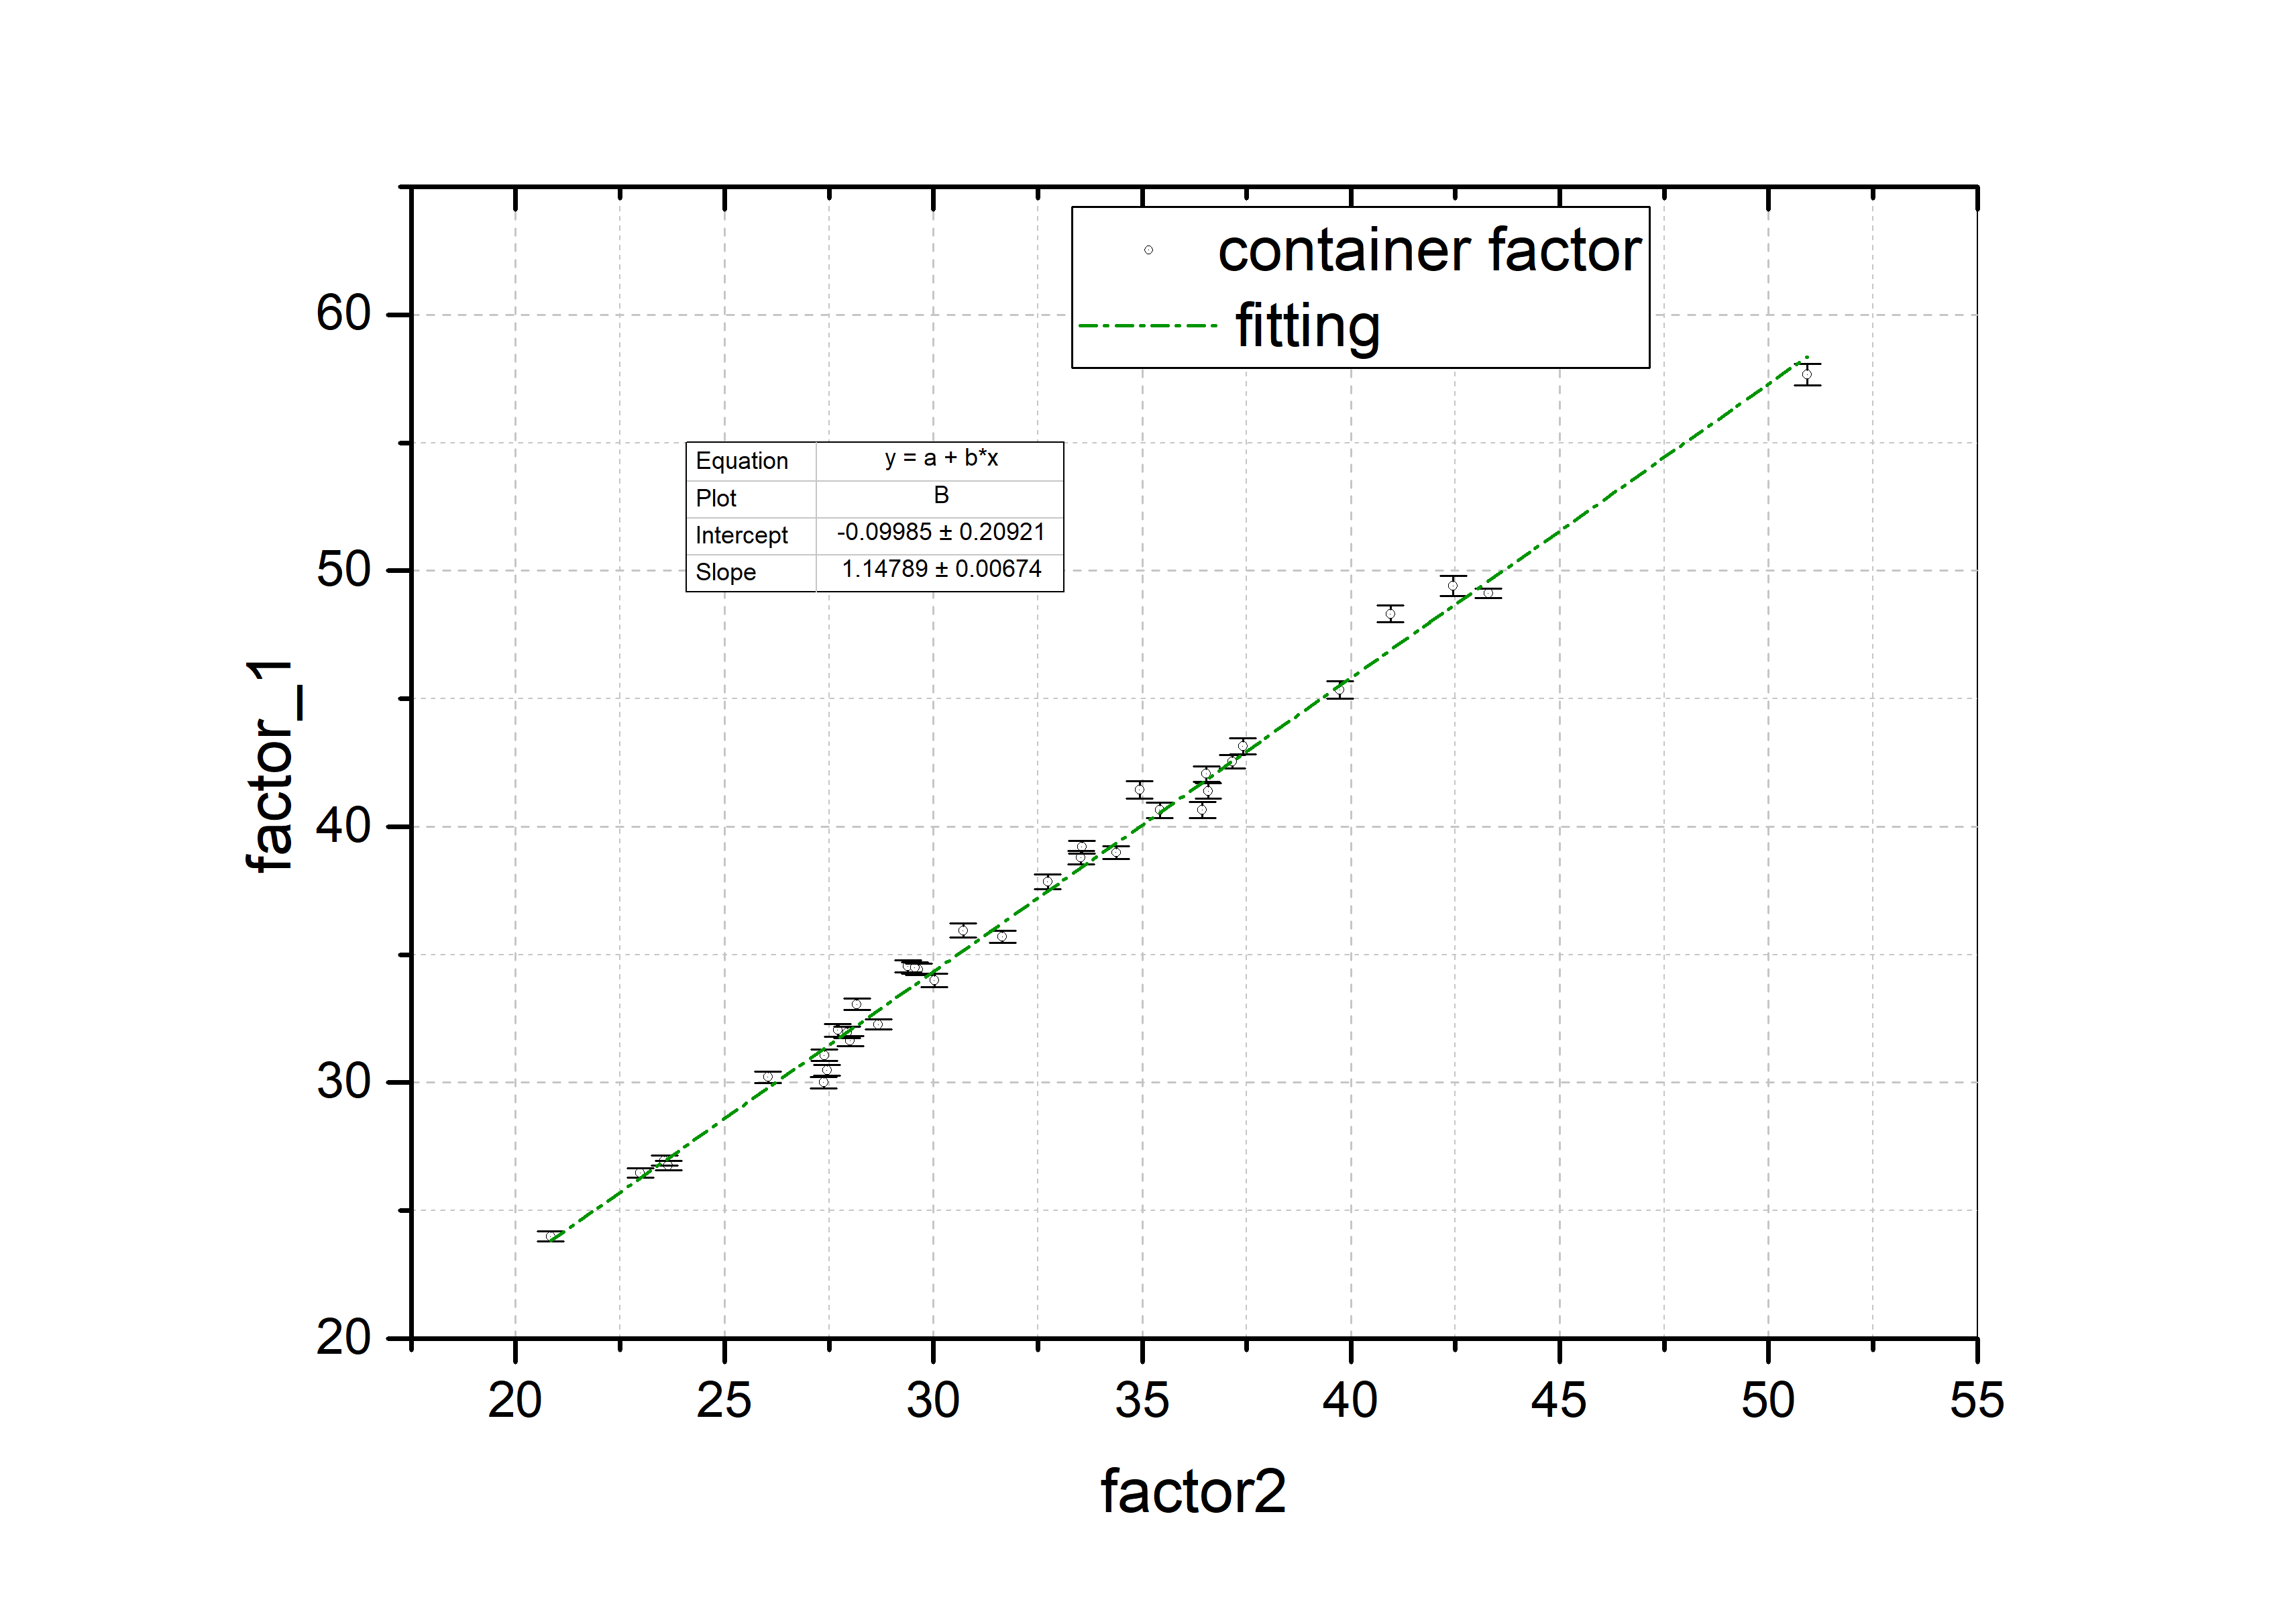
\includegraphics[width=0.72\textwidth]{drawerfactors} 
\caption{抽屉因子和现场使用值的对比}
\end{figure}
\end{frame}

\begin{frame}{两套装置测量结果的转换}
利用$PDE_c$和$PDE_s$对所有高量子效率MCP-PMT拟合$f_{cs}$的结果:
\begin{figure}
\centering
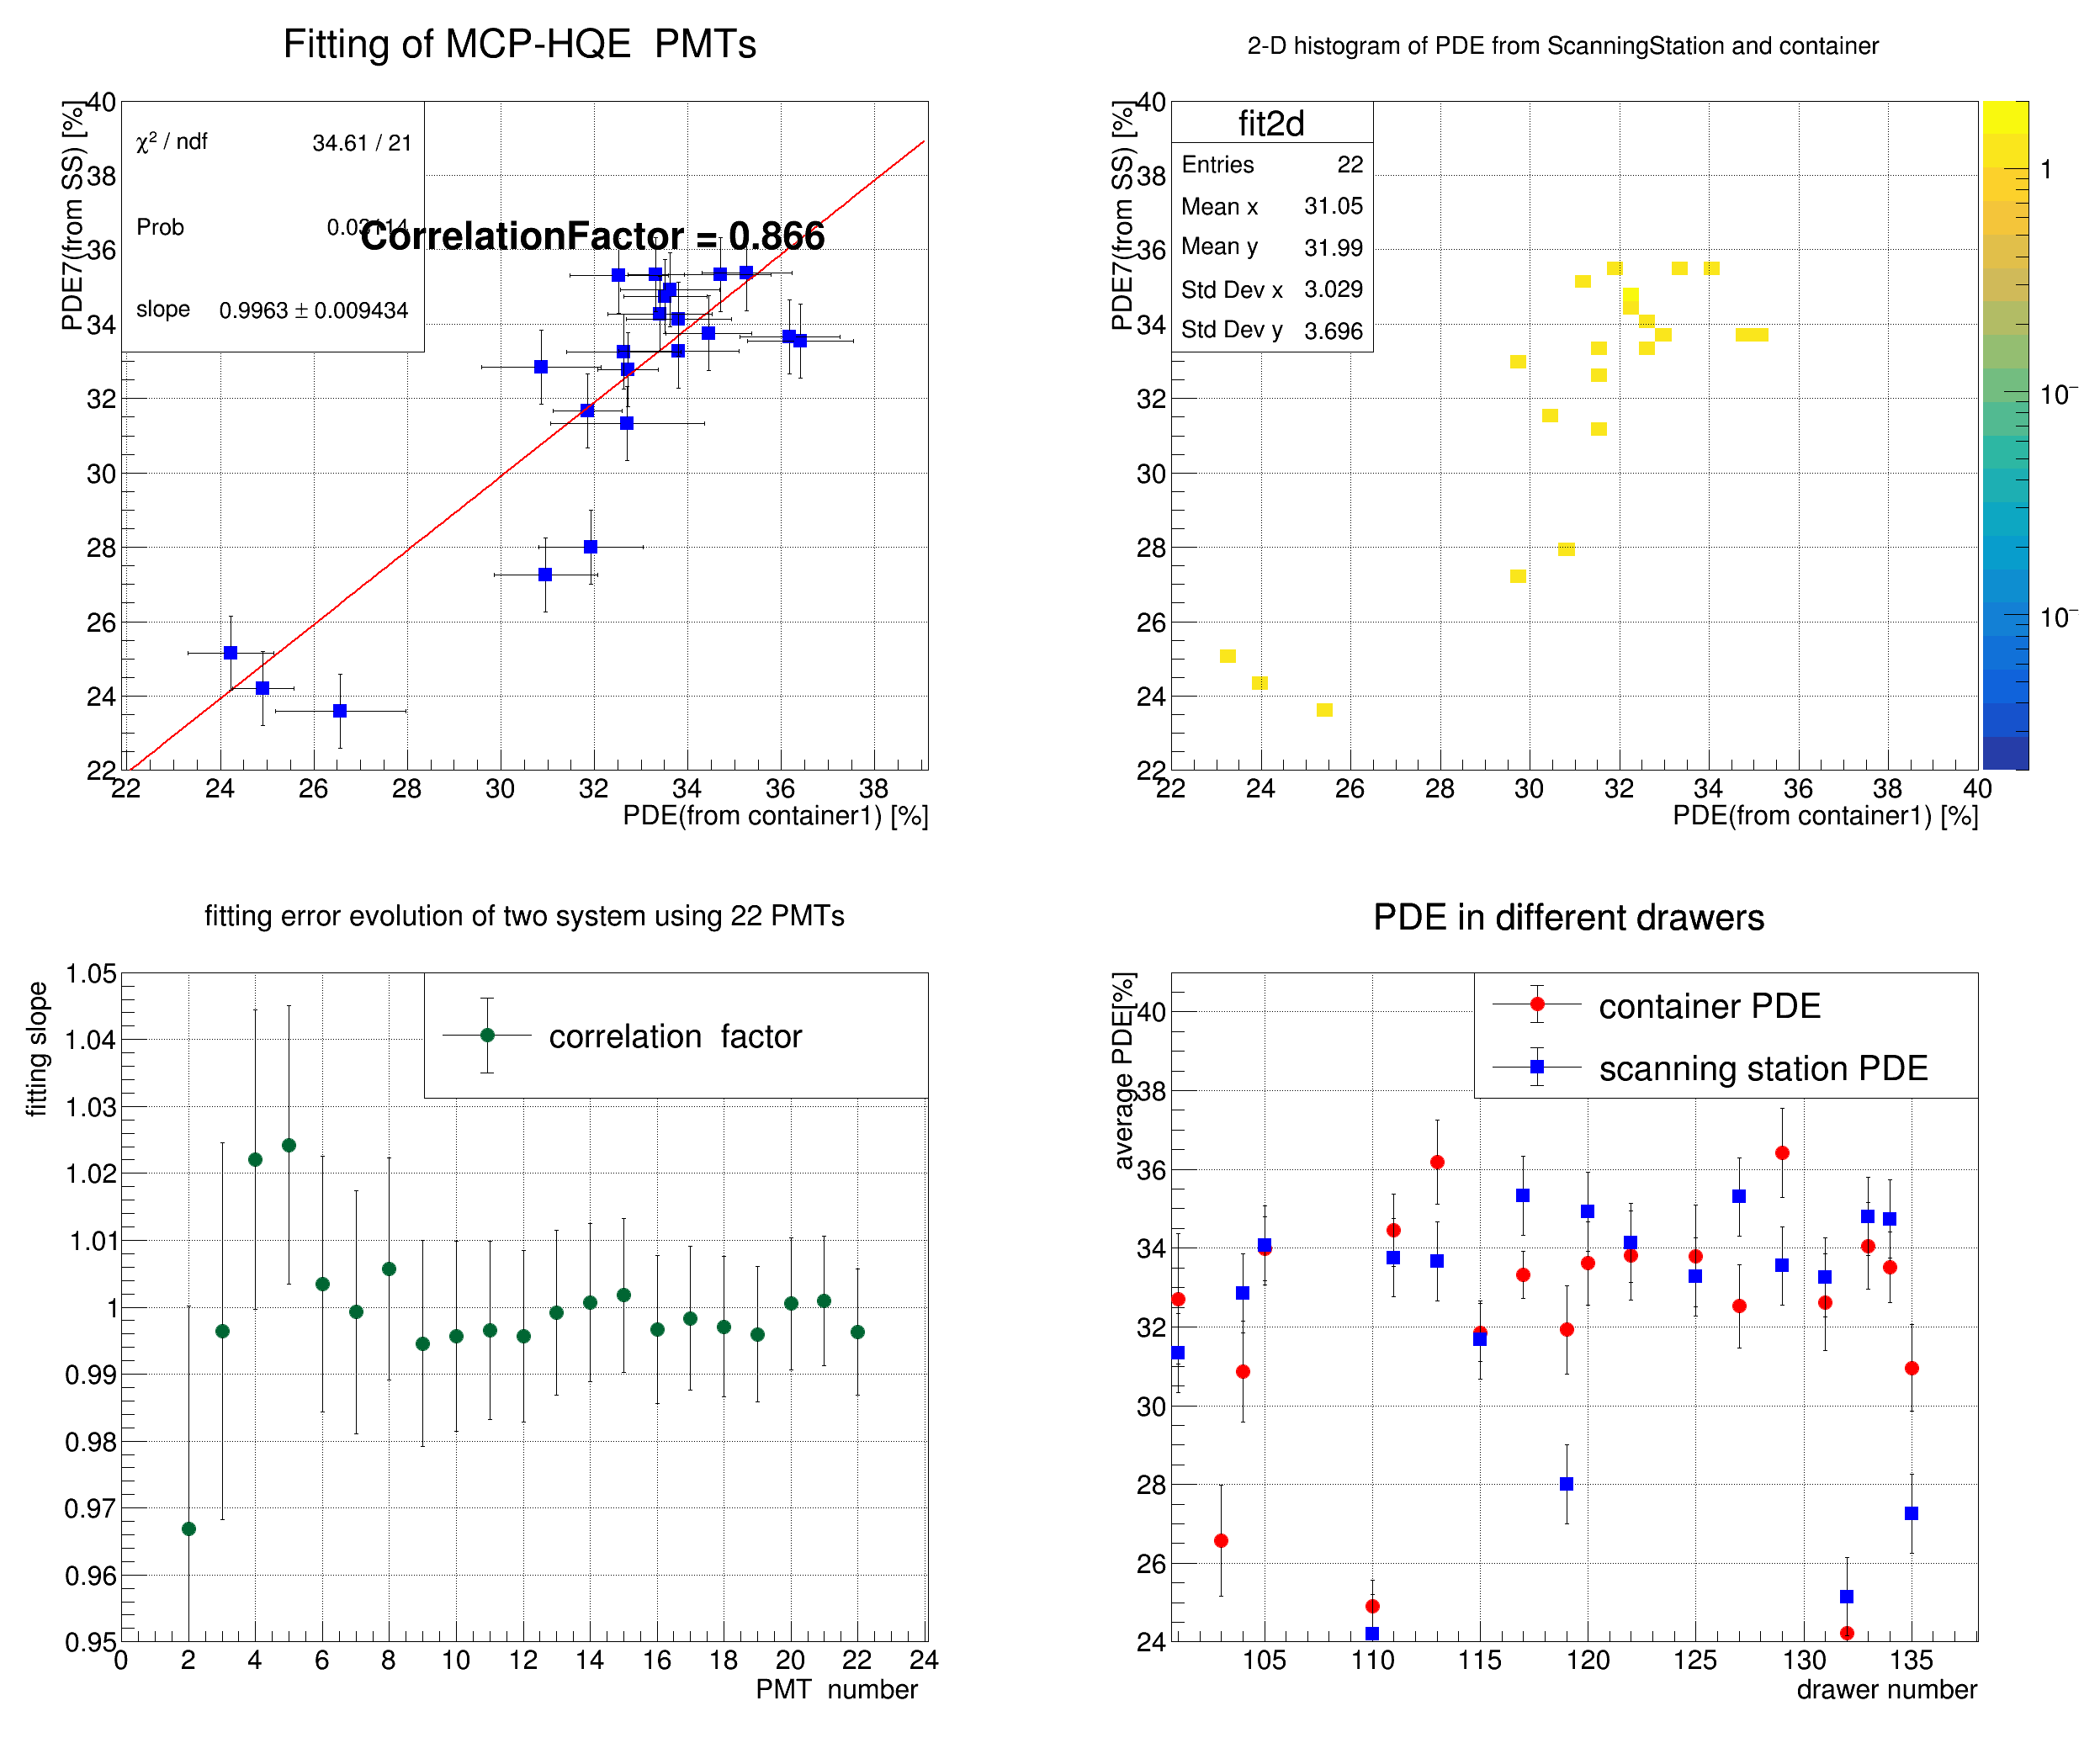
\includegraphics[width=0.68\textwidth]{fit_mcp_hqe_noint}
\end{figure}
\end{frame}
\begin{frame}{两套装置测量结果的转换}
利用$PDE_c$和$PDE_s$对所有低量子效率MCP-PMT拟合$f_{cs}$的结果:
\begin{figure}
\centering
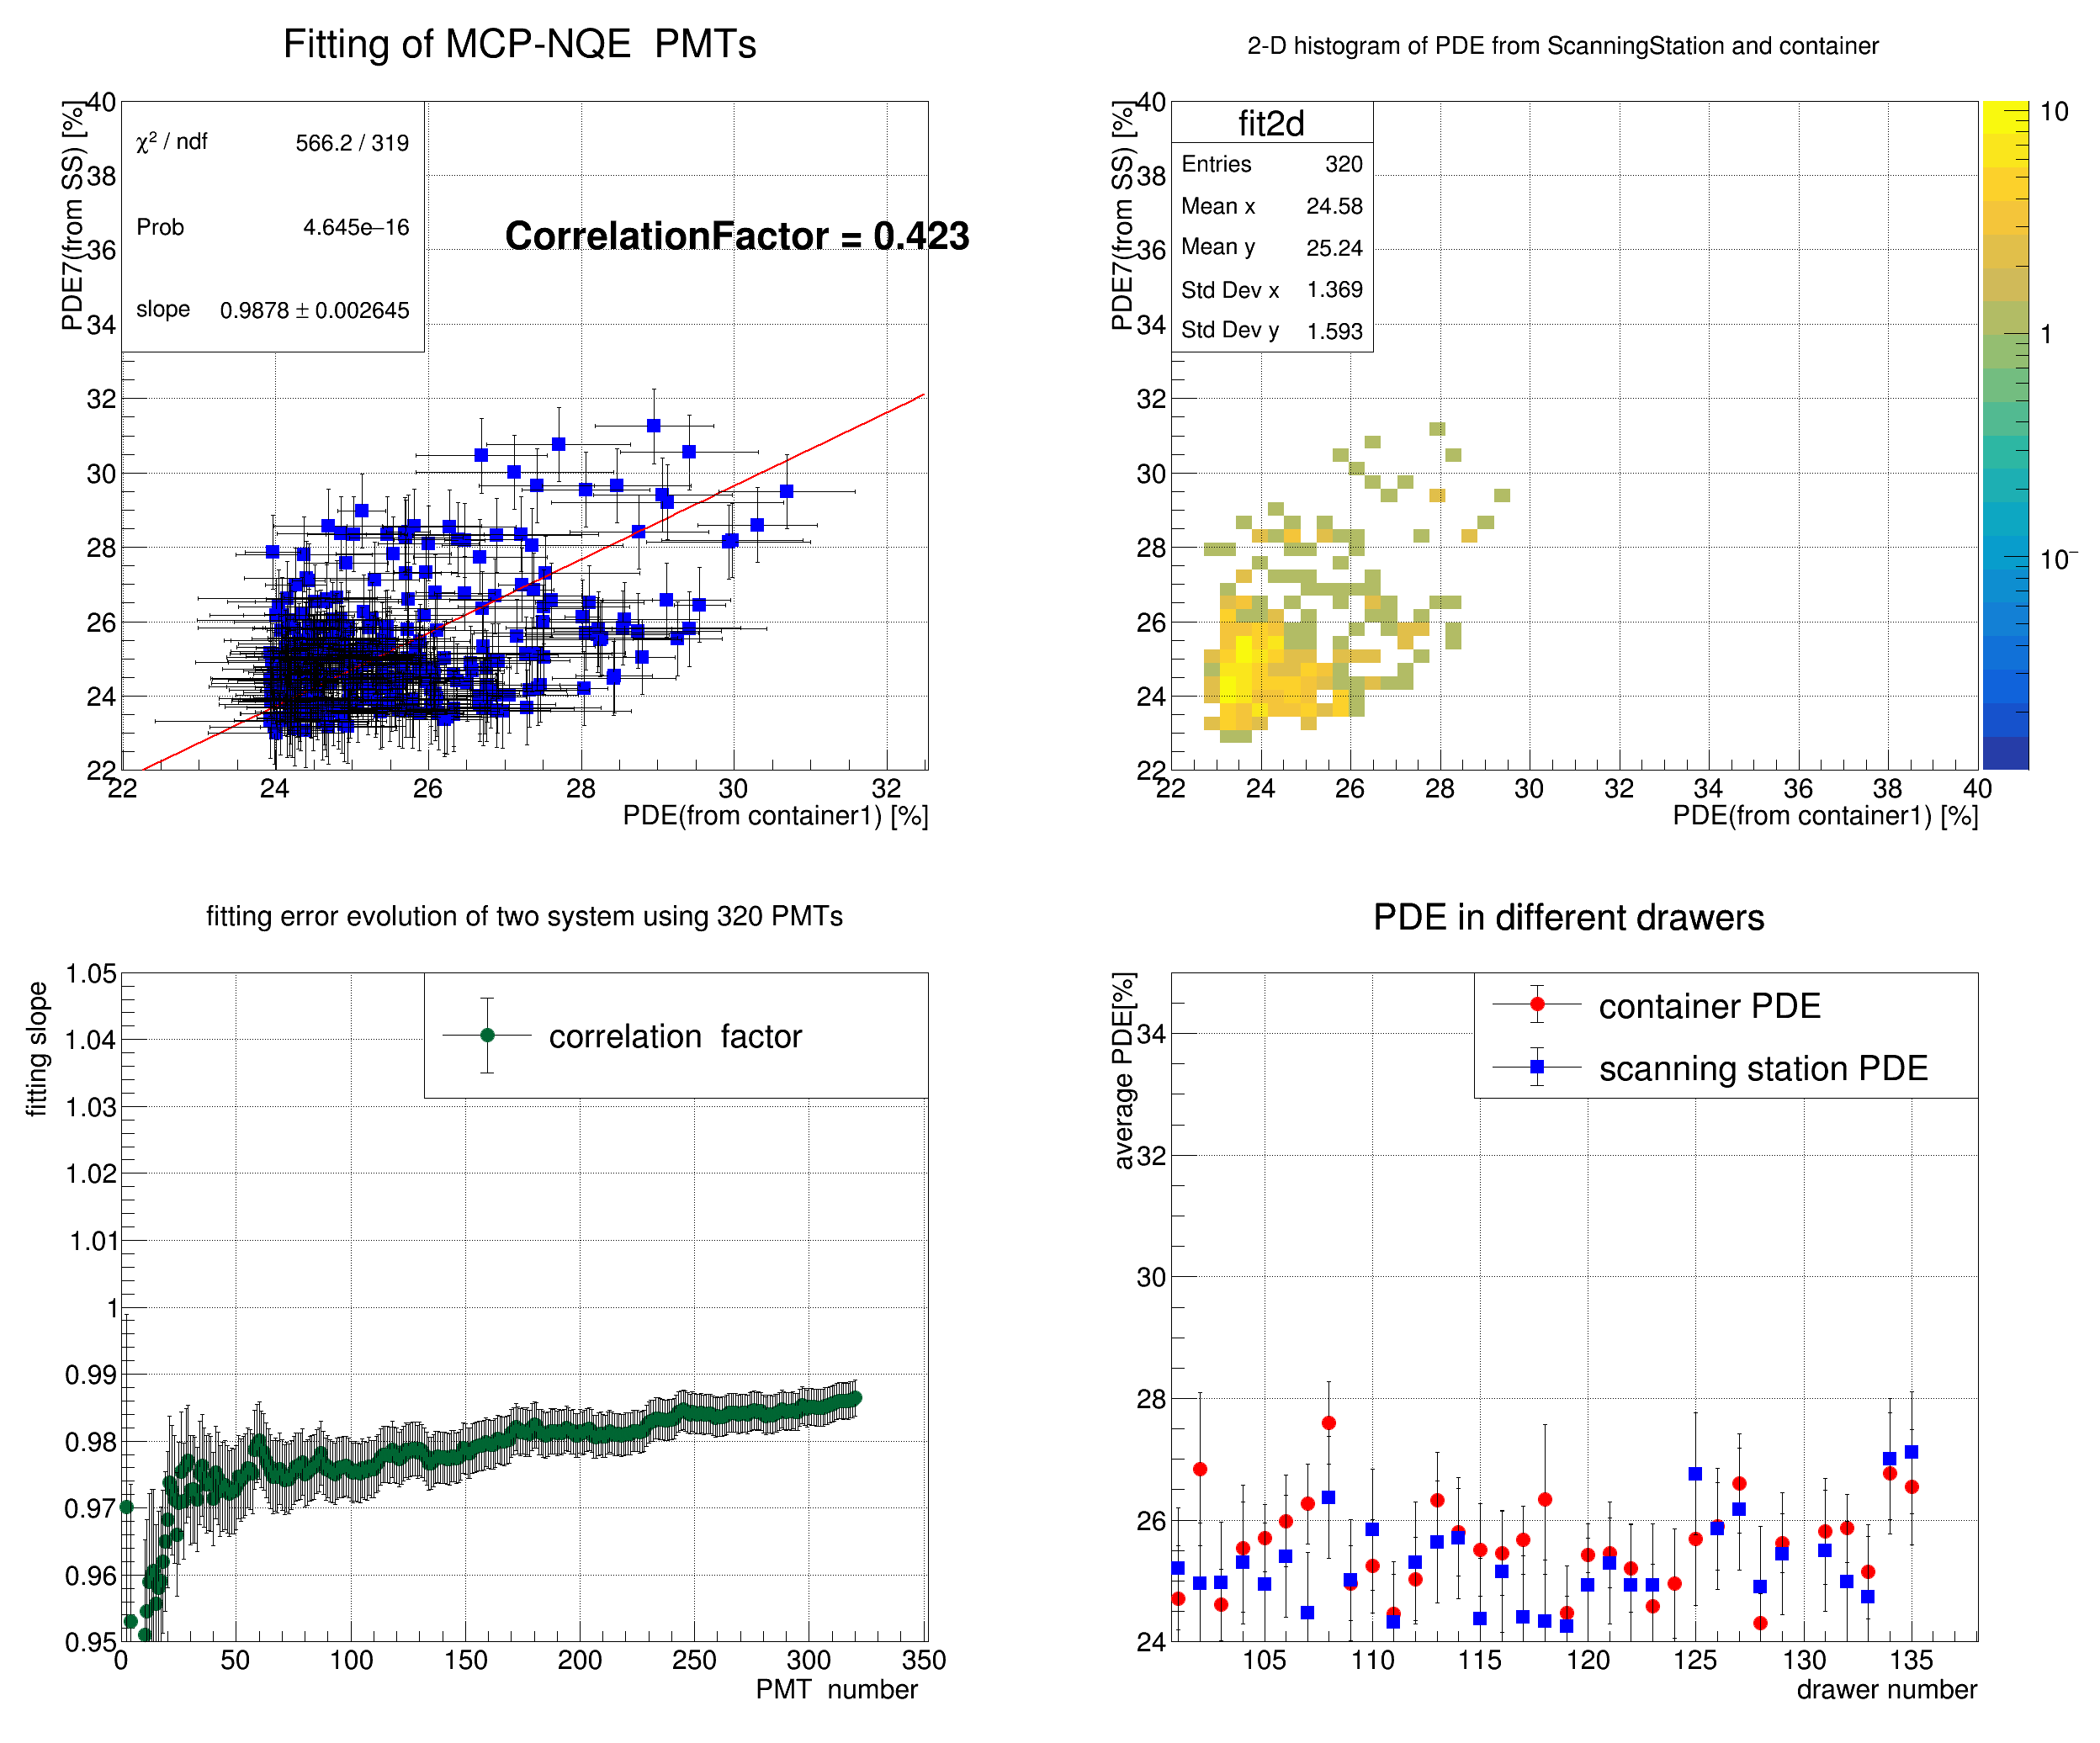
\includegraphics[width=0.68\textwidth]{fit_mcp_nqe_noint}
\end{figure}
\end{frame}
%%%%%%%%%%%%%%%%%%%%%%%%%%%%%%%%%%%%%%%%%%%
\begin{frame}{参考管稳定性}
\begin{figure}
\centering
\includegraphics[width=0.68\textwidth]{ref_sta}
\end{figure}
\end{frame}
%%%%%%%%%%%%%%%%%%%%%%%%%%%%%%%%%%%%%%%%%%%
\begin{frame}{参考管电压稳定性}
新DAQ对系统的性能产生了影响,高压平均值发生了变化:
\begin{figure}
\centering
\includegraphics[width=0.68\textwidth]{ref_HV_sta}
\end{figure}
\end{frame}
%%%%%%%%%%%%%%%%%%%%%%%%%%%%%%%%%%%%%%%%%%%
\begin{frame}{EA0419}
参考管EA0419一直在101抽屉,它的测量结果反映了集装箱测试系统的性能和稳定性:
\begin{figure}
\centering
\includegraphics[width=0.98\textwidth]{101_sta}
\end{figure}
\end{frame}
%%%%%%%%%%%%%%%%%%%%%%%%%%%%%%%%%%%%%%%%%%%
\begin{frame}{暗计数}
\begin{figure}
\centering
\includegraphics[width=0.48\textwidth]{vendordcr_mcp}
\includegraphics[width=0.48\textwidth]{vendordcr_hmp}
\end{figure}
\end{frame}
%%%%%%%%%%%%%%%%%%%%%%%%%%%%%%%%%%%%%%%%%%%
\begin{frame}{上升时间和下降时间分布}
\begin{figure}
\centering
\includegraphics[width=0.48\textwidth]{risetime}
\includegraphics[width=0.48\textwidth]{falltime}
\end{figure}
\end{frame}
%%%%%%%%%%%%%%%%%%%%%%%%%%%%%%%%%%%%%%%%%%%
\begin{frame}{峰谷比和SPE分辨率分布}
\begin{figure}
\centering
\includegraphics[width=0.48\textwidth]{pvr}
\includegraphics[width=0.48\textwidth]{resolution}
\end{figure}
\end{frame}
%%%%%%%%%%%%%%%%%%%%%%%%%%%%%%%%%%%%%%%%%%%
\begin{frame}{增益和FWHM的对比}
\begin{figure}
\centering
\includegraphics[width=0.48\textwidth]{gain}
\includegraphics[width=0.48\textwidth]{fwhm}
\end{figure}
\end{frame}
%%%%%%%%%%%%%%%%%%%%%%%%%%%%%%%%%%%%%%%%%%%
\begin{frame}{平均PDE}
每个抽屉的平均PDE分布:
\begin{figure}
\centering
\includegraphics[width=0.88\textwidth]{dpde}
\end{figure}
\end{frame}
%% OpenBUGS  WinBUGS  JAGS
% library(R2OpenBUGS) # 2017-2-20 version 3.2-3.2
% library(R2WinBUGS) # 2015-07-29 version 2.1-21
% library(rjags) # 2016-02-19 version 4-6
% library(BRugs) # OpenBUGS 2017-06-26  version 0.9-0
% library(glmmBUGS) # Generalised Linear Mixed Models with BUGS and JAGS 2016-09-22 version 2.4.0
% library(R2jags) # Using R to Run 'JAGS'  2015-08-23	 version 0.5-7

% network
	% diagram DiagrammeR DiagrammeRsvg
 % library(help=graph)

 % library(help=Rgraphviz)
 % library(help=igraph)


%\begin{frame}{Ack}
%\begin{itemize}
%\item[\faGithub] \href{https://github.com/Cloud2016}{Cloud2016} \faAt Github
%\item[\aiOverleaf] \href{https://www.overleaf.com/}{Xiangyun} \faAt Overleaf
%\item[\aiarXiv] \href{https://arxiv.org/}{arXiv}
%\end{itemize}
%\end{frame}

\end{document} 


